\documentclass[12pt]{article}
\usepackage{amsmath}
\usepackage{latexsym}
\usepackage{amsfonts}
\usepackage[normalem]{ulem}
\usepackage{soul}
\usepackage{array}
\usepackage{amssymb}
\usepackage{extarrows}
\usepackage{graphicx}

\usepackage[backend=biber,
style=numeric,
sorting=none,
isbn=false,
doi=false,
url=false,
]{biblatex}\addbibresource{bibliography.bib}

\usepackage{subfig}
\usepackage{wrapfig}
\usepackage{wasysym}
\usepackage{enumitem}
\usepackage{adjustbox}
\usepackage{ragged2e}
\usepackage[svgnames,table]{xcolor}
\usepackage{tikz}
\usepackage{longtable}
\usepackage{changepage}
\usepackage{setspace}
\usepackage{hhline}
\usepackage{multicol}
\usepackage{tabto}
\usepackage{float}
\usepackage{multirow}
\usepackage{makecell}
\usepackage{fancyhdr}
\usepackage[toc,page]{appendix}
\usepackage[hidelinks]{hyperref}
\usetikzlibrary{shapes.symbols,shapes.geometric,shadows,arrows.meta}
\tikzset{>={Latex[width=1.5mm,length=2mm]}}
\usepackage{flowchart}
\usepackage[paperheight=11.0in,paperwidth=8.5in,left=1.0in,right=1.0in,top=1.0in,bottom=1.0in,headheight=1in]{geometry}
\usepackage[utf8]{inputenc}
\usepackage[T1]{fontenc}
\TabPositions{0.5in,1.0in,1.5in,2.0in,2.5in,3.0in,3.5in,4.0in,4.5in,5.0in,5.5in,6.0in,}

\urlstyle{same}

\renewcommand{\baselinestretch}{1.3}

\renewcommand{\_}{\kern-1.5pt\textunderscore\kern-1.5pt}



\setcounter{tocdepth}{5}
\setcounter{secnumdepth}{5}


 %%%%%%%%%%%%  Set Depths for Nested Lists created by \begin{enumerate}  %%%%%%%%%%%%%%
\captionsetup[subfigure]{font=footnotesize}


\setlistdepth{9}
\renewlist{enumerate}{enumerate}{9}
		\setlist[enumerate,1]{label=\arabic*)}
		\setlist[enumerate,2]{label=\alph*)}
		\setlist[enumerate,3]{label=(\roman*)}
		\setlist[enumerate,4]{label=(\arabic*)}
		\setlist[enumerate,5]{label=(\Alph*)}
		\setlist[enumerate,6]{label=(\Roman*)}
		\setlist[enumerate,7]{label=\arabic*}
		\setlist[enumerate,8]{label=\alph*}
		\setlist[enumerate,9]{label=\roman*}

\renewlist{itemize}{itemize}{9}
		\setlist[itemize]{label=$\cdot$}
		\setlist[itemize,1]{label=\textbullet}
		\setlist[itemize,2]{label=$\circ$}
		\setlist[itemize,3]{label=$\ast$}
		\setlist[itemize,4]{label=$\dagger$}
		\setlist[itemize,5]{label=$\triangleright$}
		\setlist[itemize,6]{label=$\bigstar$}
		\setlist[itemize,7]{label=$\blacklozenge$}
		\setlist[itemize,8]{label=$\prime$}

\setlength{\topsep}{0pt}\setlength{\parskip}{8.04pt}
\setlength{\parindent}{0pt}



\renewcommand{\arraystretch}{1.3}

\title{SoliGity}
\author{  Roger Luo
  \and
  Zhenpeng Wu\\
  28125152 
  \and
  Daniel Tong
}

\date{\today}





\begin{document}

\maketitle



\vspace{\baselineskip}
\begin{enumerate}
	\item Introduction\par

The course project of EECE571G is to let you try your best to build a decentralized application (DApp). As this is graduate course, students are expected to form a software development team to do this project. \par

	\item Requirement\par

\begin{enumerate}
	\item Team Building\par

\begin{enumerate}
	\item The project is a team-based project (i.e. group project). We have 3 $ \sim $  5 students in each team. A team should have at least 3 students. \par

	\item Please print the team form given you in the appendix of this document out and the members of each team need to fill the form and give their signatures properly. The team should submit the form in the midterm week.\par

	\item Certainly, every student can join at most one group. \par


\end{enumerate}
	\item Contents\par

\begin{enumerate}
	\item Think about a simple application to develop with the blockchain technology.\  \par

	\item Setup the development environment \par

The team needs to setup the \textbf{\uline{Truffle + React + Web3js}} development environments. \par

	\item Each group should create a project on GitHub and put your project on the GitHub. In the end of the term, please send me the link of your project repository on GitHub. \par

	\item Your project should be runnable and functional.\par

	\item In your Assignment 2 (which is group based), please submit the follows:\par

\begin{enumerate}
	\item \textbf{\uline{The whitepaper}} of your project (i.e., a document describes the application). \par

	\item The \textbf{\uline{wireframe}}.\par

	\item The \textbf{\uline{smart contract code}}.\par

	\item The \textbf{\uline{test code for your smart contract}}.\par


\end{enumerate}
	\item Project demo and final report submission are needed in the end.\par


\end{enumerate}
\end{enumerate}
	\item Evaluation\par

\begin{enumerate}
	\item Presentation\par

In the \textbf{\uline{very last week}}, we have a presentation course. The presentation takes 70$\%$  of your project evaluation. \par

	\item Report\par

The report should be at least 20 pages of main contents in Letter paper, Font Size = 12, 1.5 times line spacing, with Normal margin in \textbf{\uline{MS Word}} (2.54 cm for all sides). Pictures (like screenshots) are encouraged in the report, but the number of pictures cannot exceed 15 and the size of picture should meet the following requirements (Height < 8cm and Width < 14cm).\par

\textbf{\uline{Violation with any of the above rules may result in the deduction of your project marks}}.\par

	\item Fairness\par

Each team should fill in a Peer-to-Peer evaluation form for fairness purposes.\par

Each team member will receive the inner-team evaluation for his/her contributions of the course project in a percentage. That is, the sum of all members’ percentage marks \textbf{\uline{should NOT exceed 100}}$\%$ , and ALL team member should sign clearly to show that they have reached an agreement.\par

If the sum of percentages over all team members exceeds 100$\%$  OR any student’s signature is missing, the form is INVALID. The form should be submitted together with the course project report on the project presentation day.\par


\vspace{\baselineskip}

\end{enumerate}
	\item Appendix (Two forms in next two pages): 


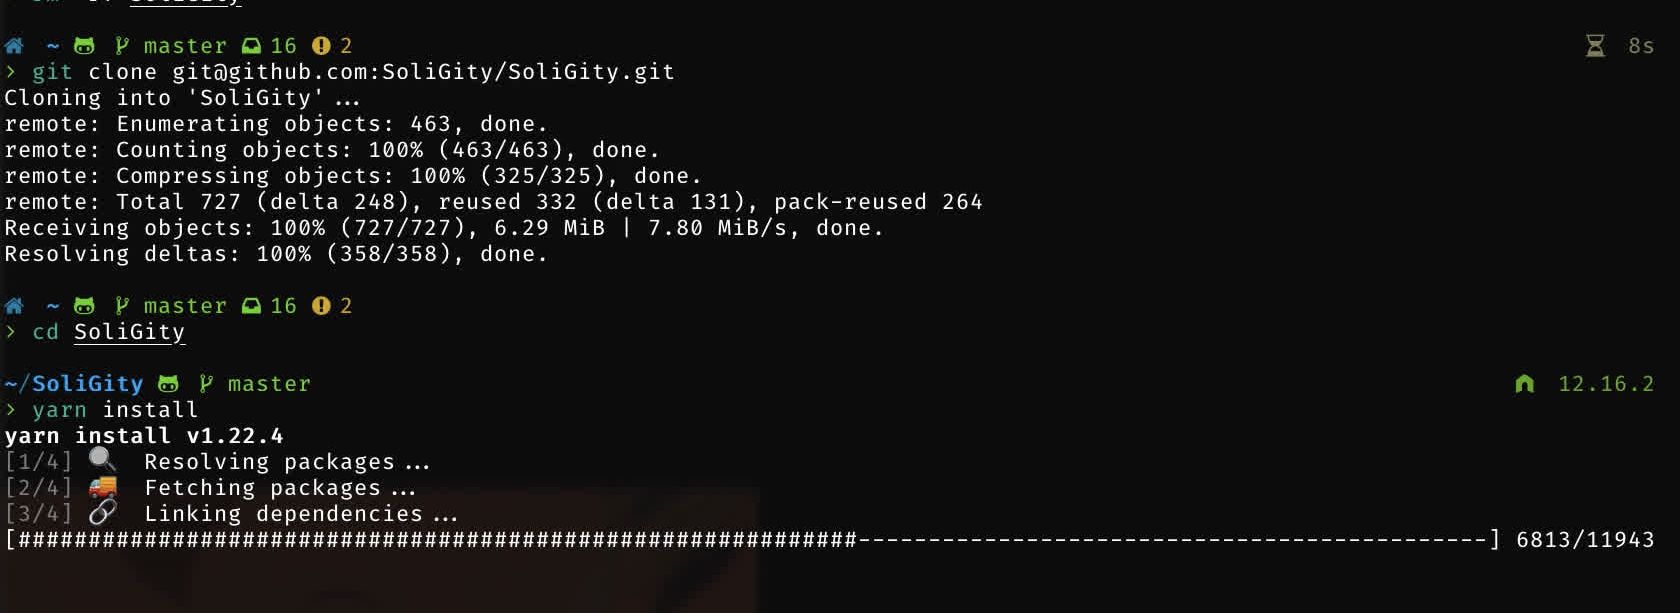
\includegraphics[height=7cm]{graphs/01. git_clone}

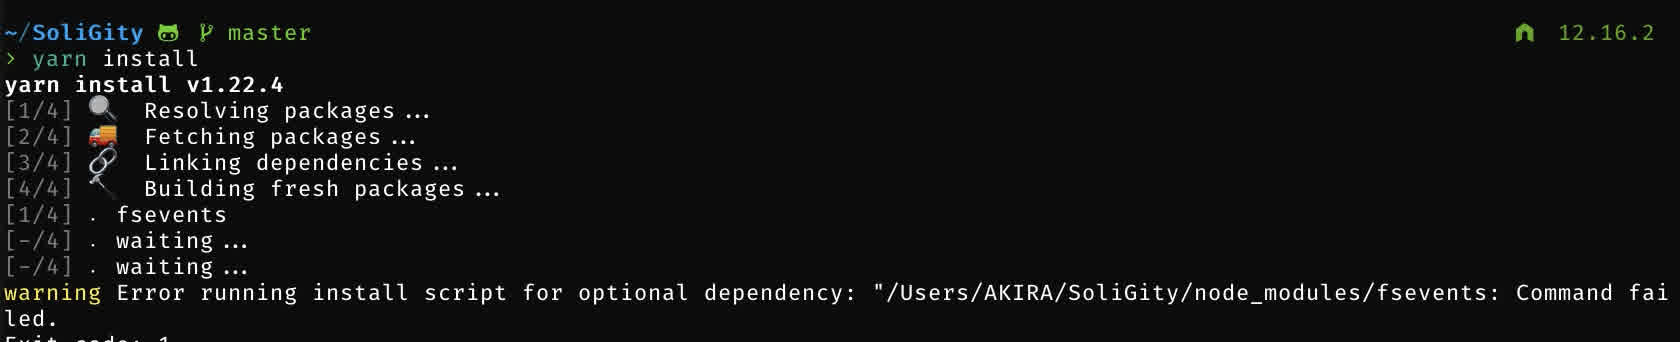
\includegraphics[height=7cm]{graphs/02. yarn_install_backend}

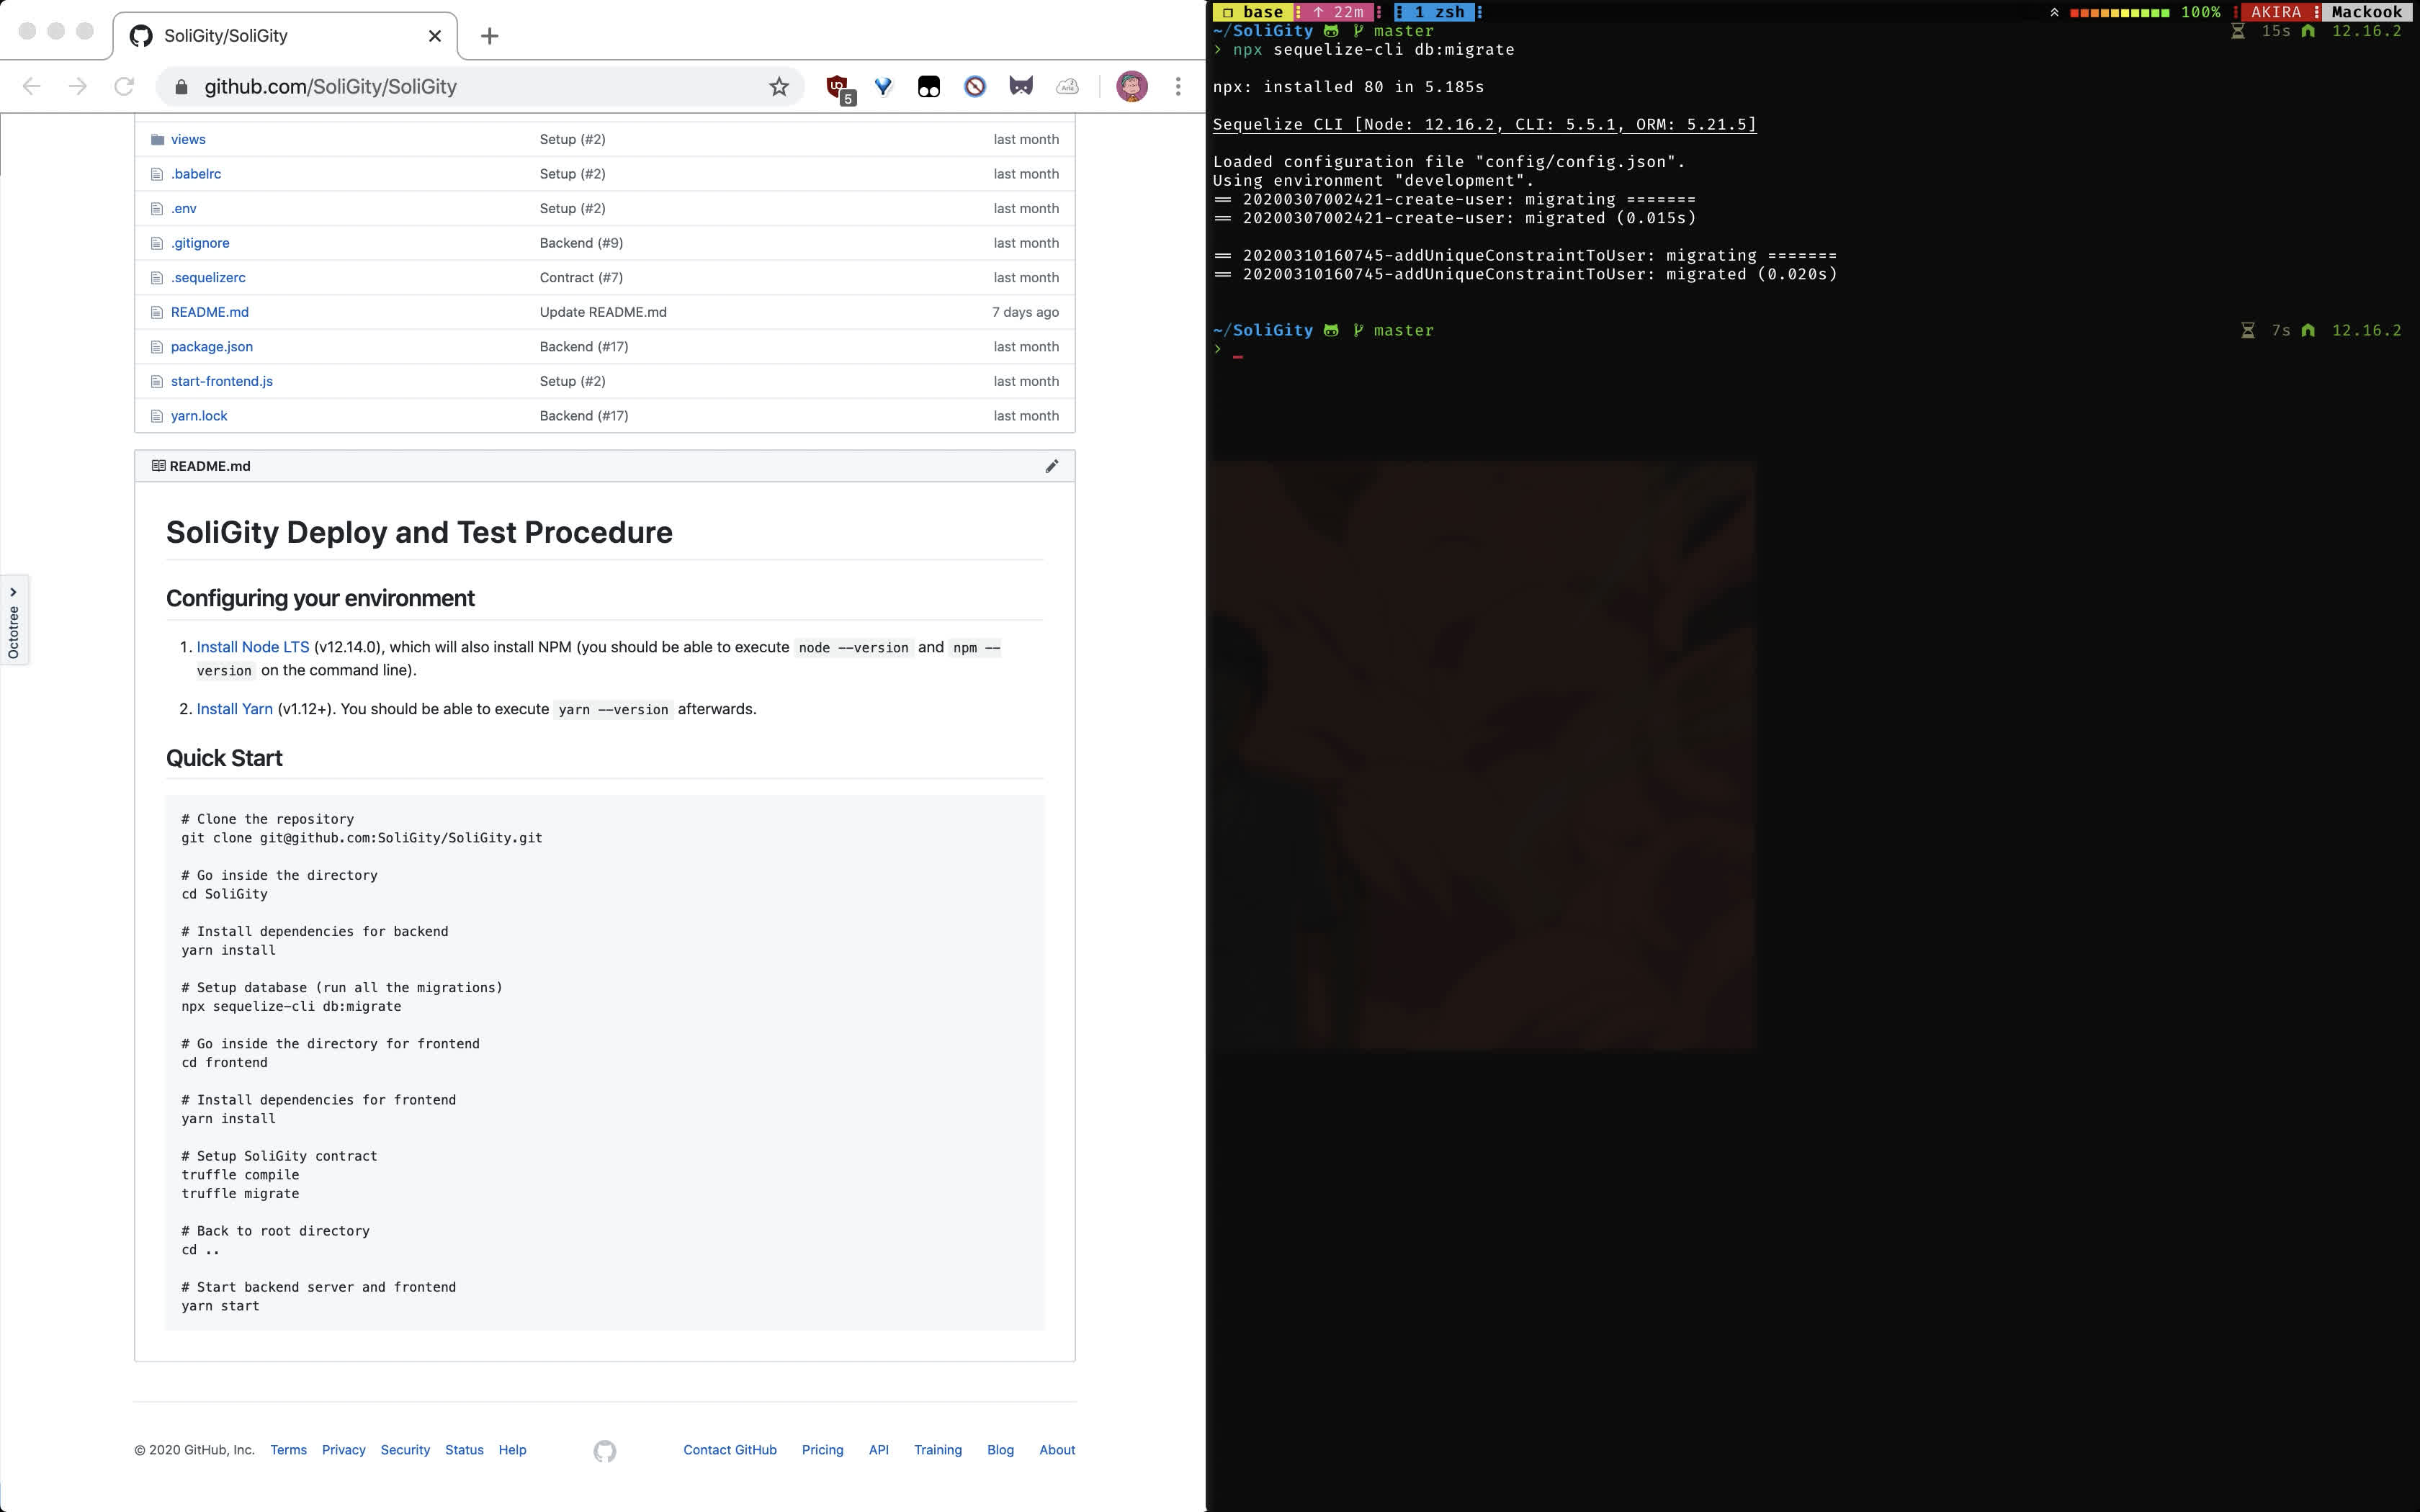
\includegraphics[height=7cm]{graphs/03. user_db_migrate} 

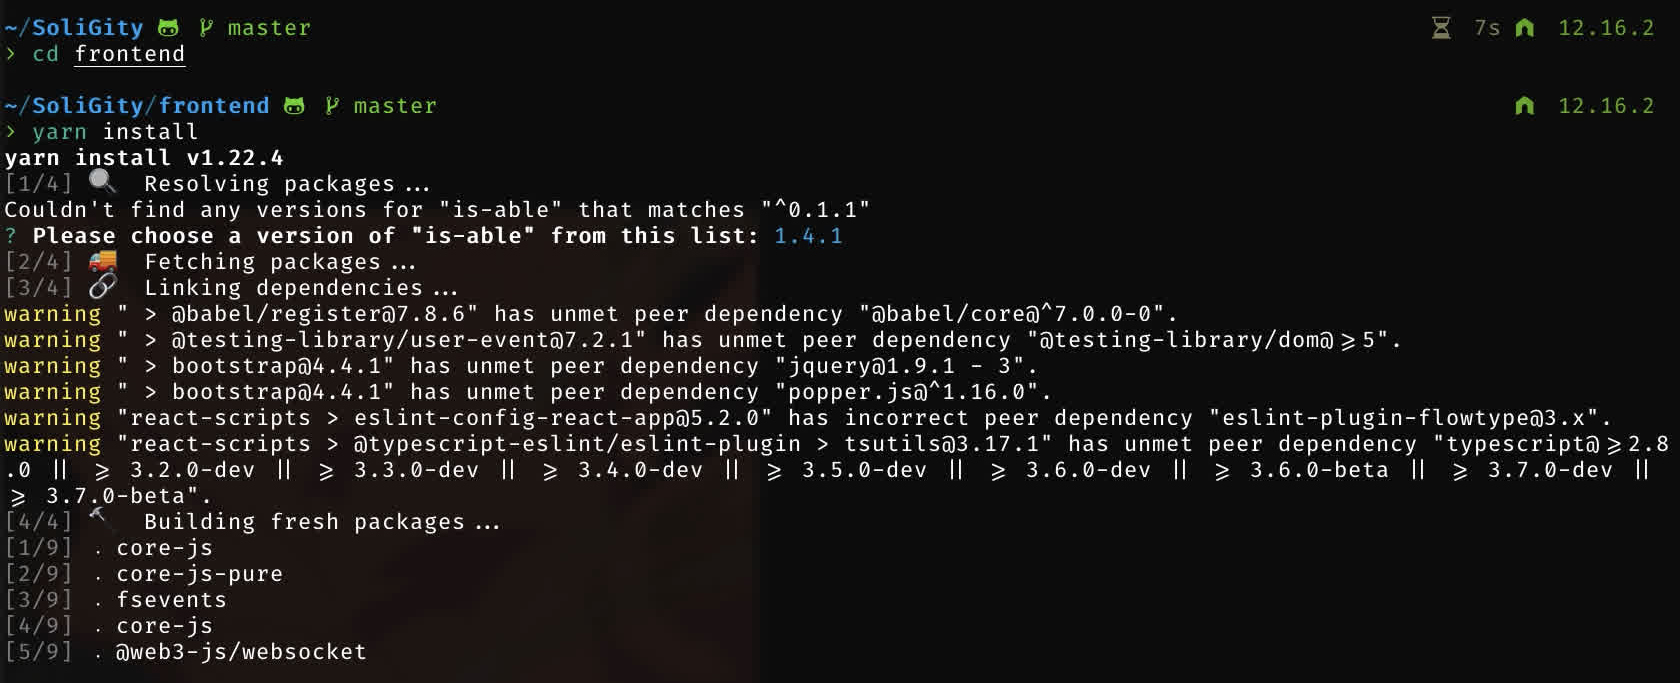
\includegraphics[height=7cm]{graphs/04. yarn_install_frontend}

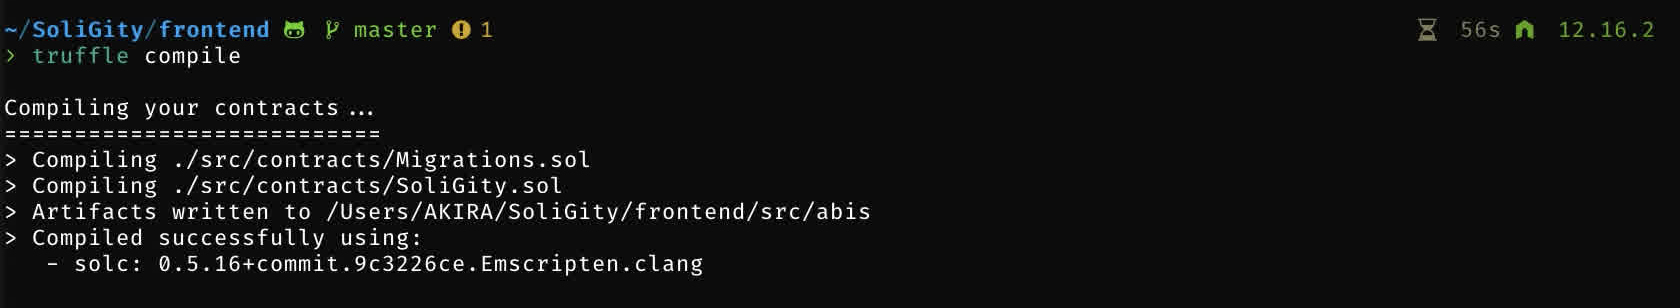
\includegraphics[height=7cm]{graphs/05. truffle_compile}

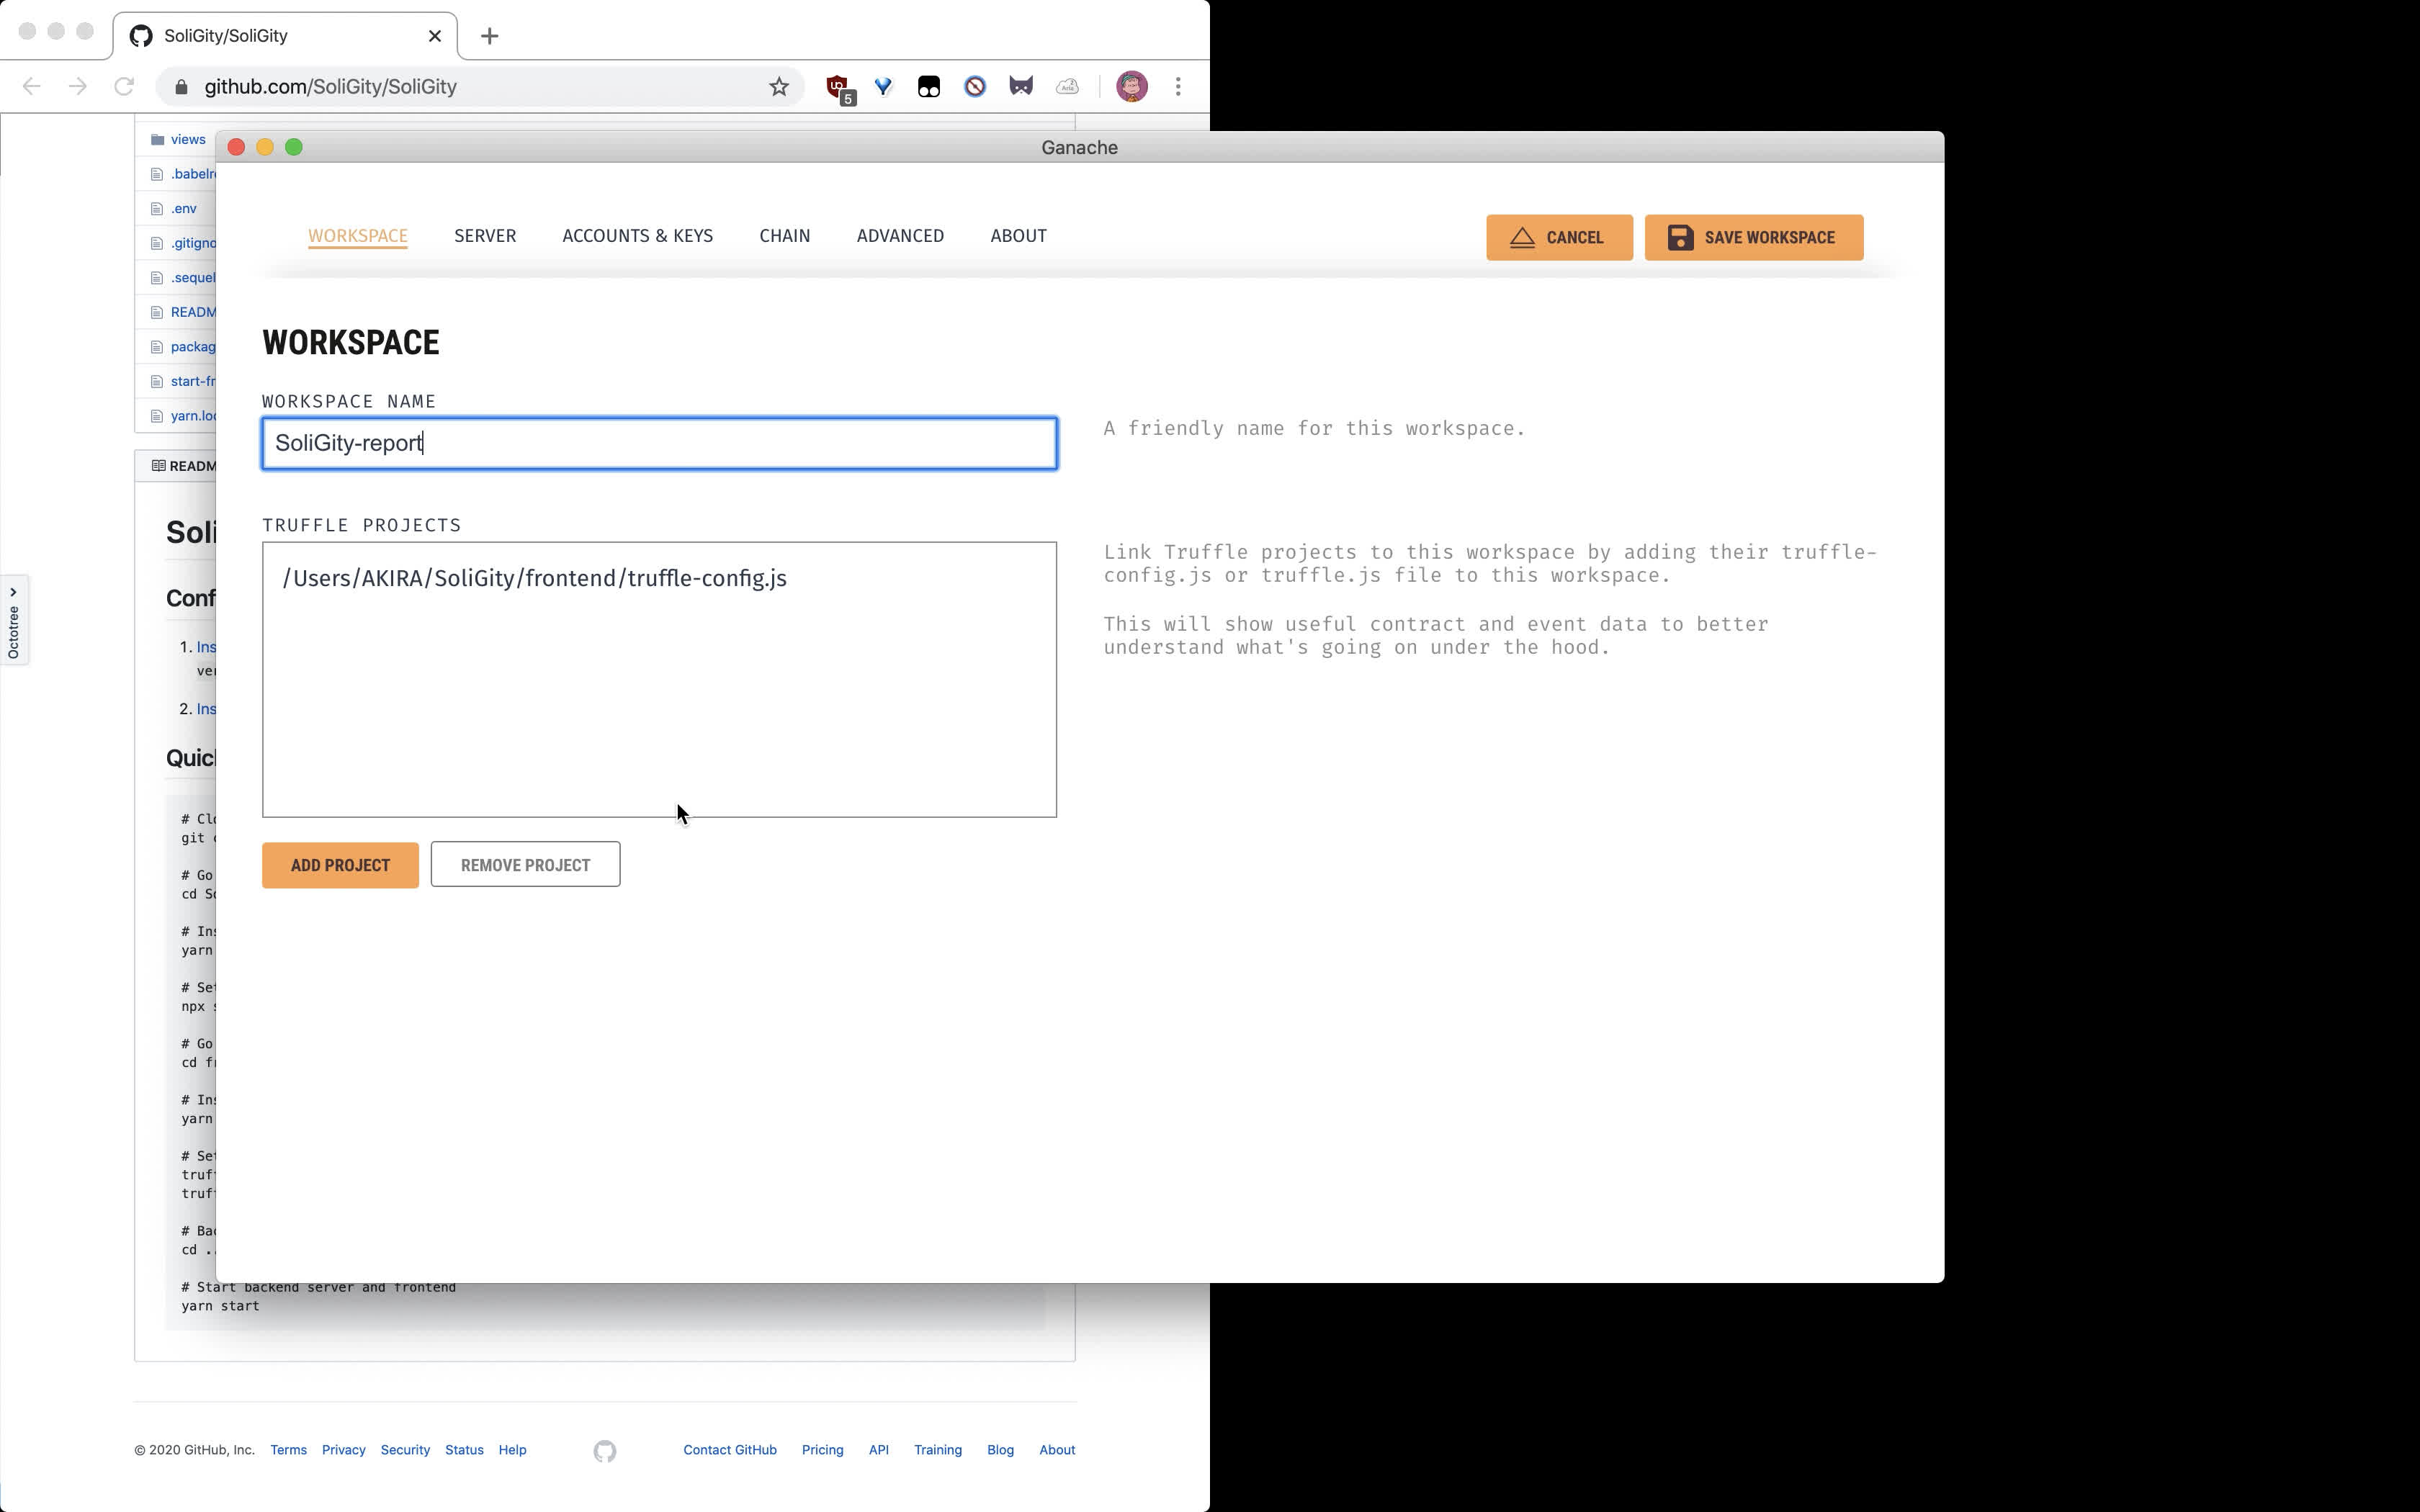
\includegraphics[height=7cm]{graphs/06. ganache_setup}

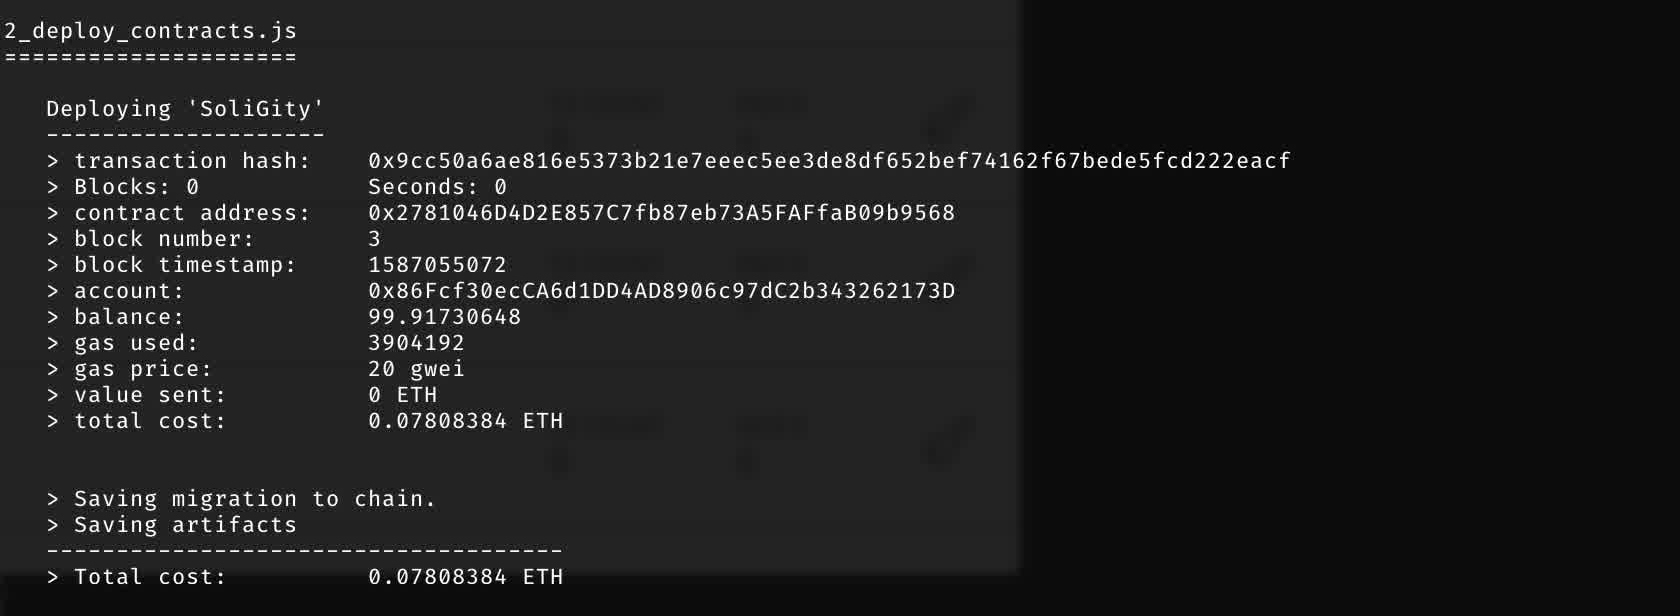
\includegraphics[height=7cm]{graphs/07. truffle_migrate}

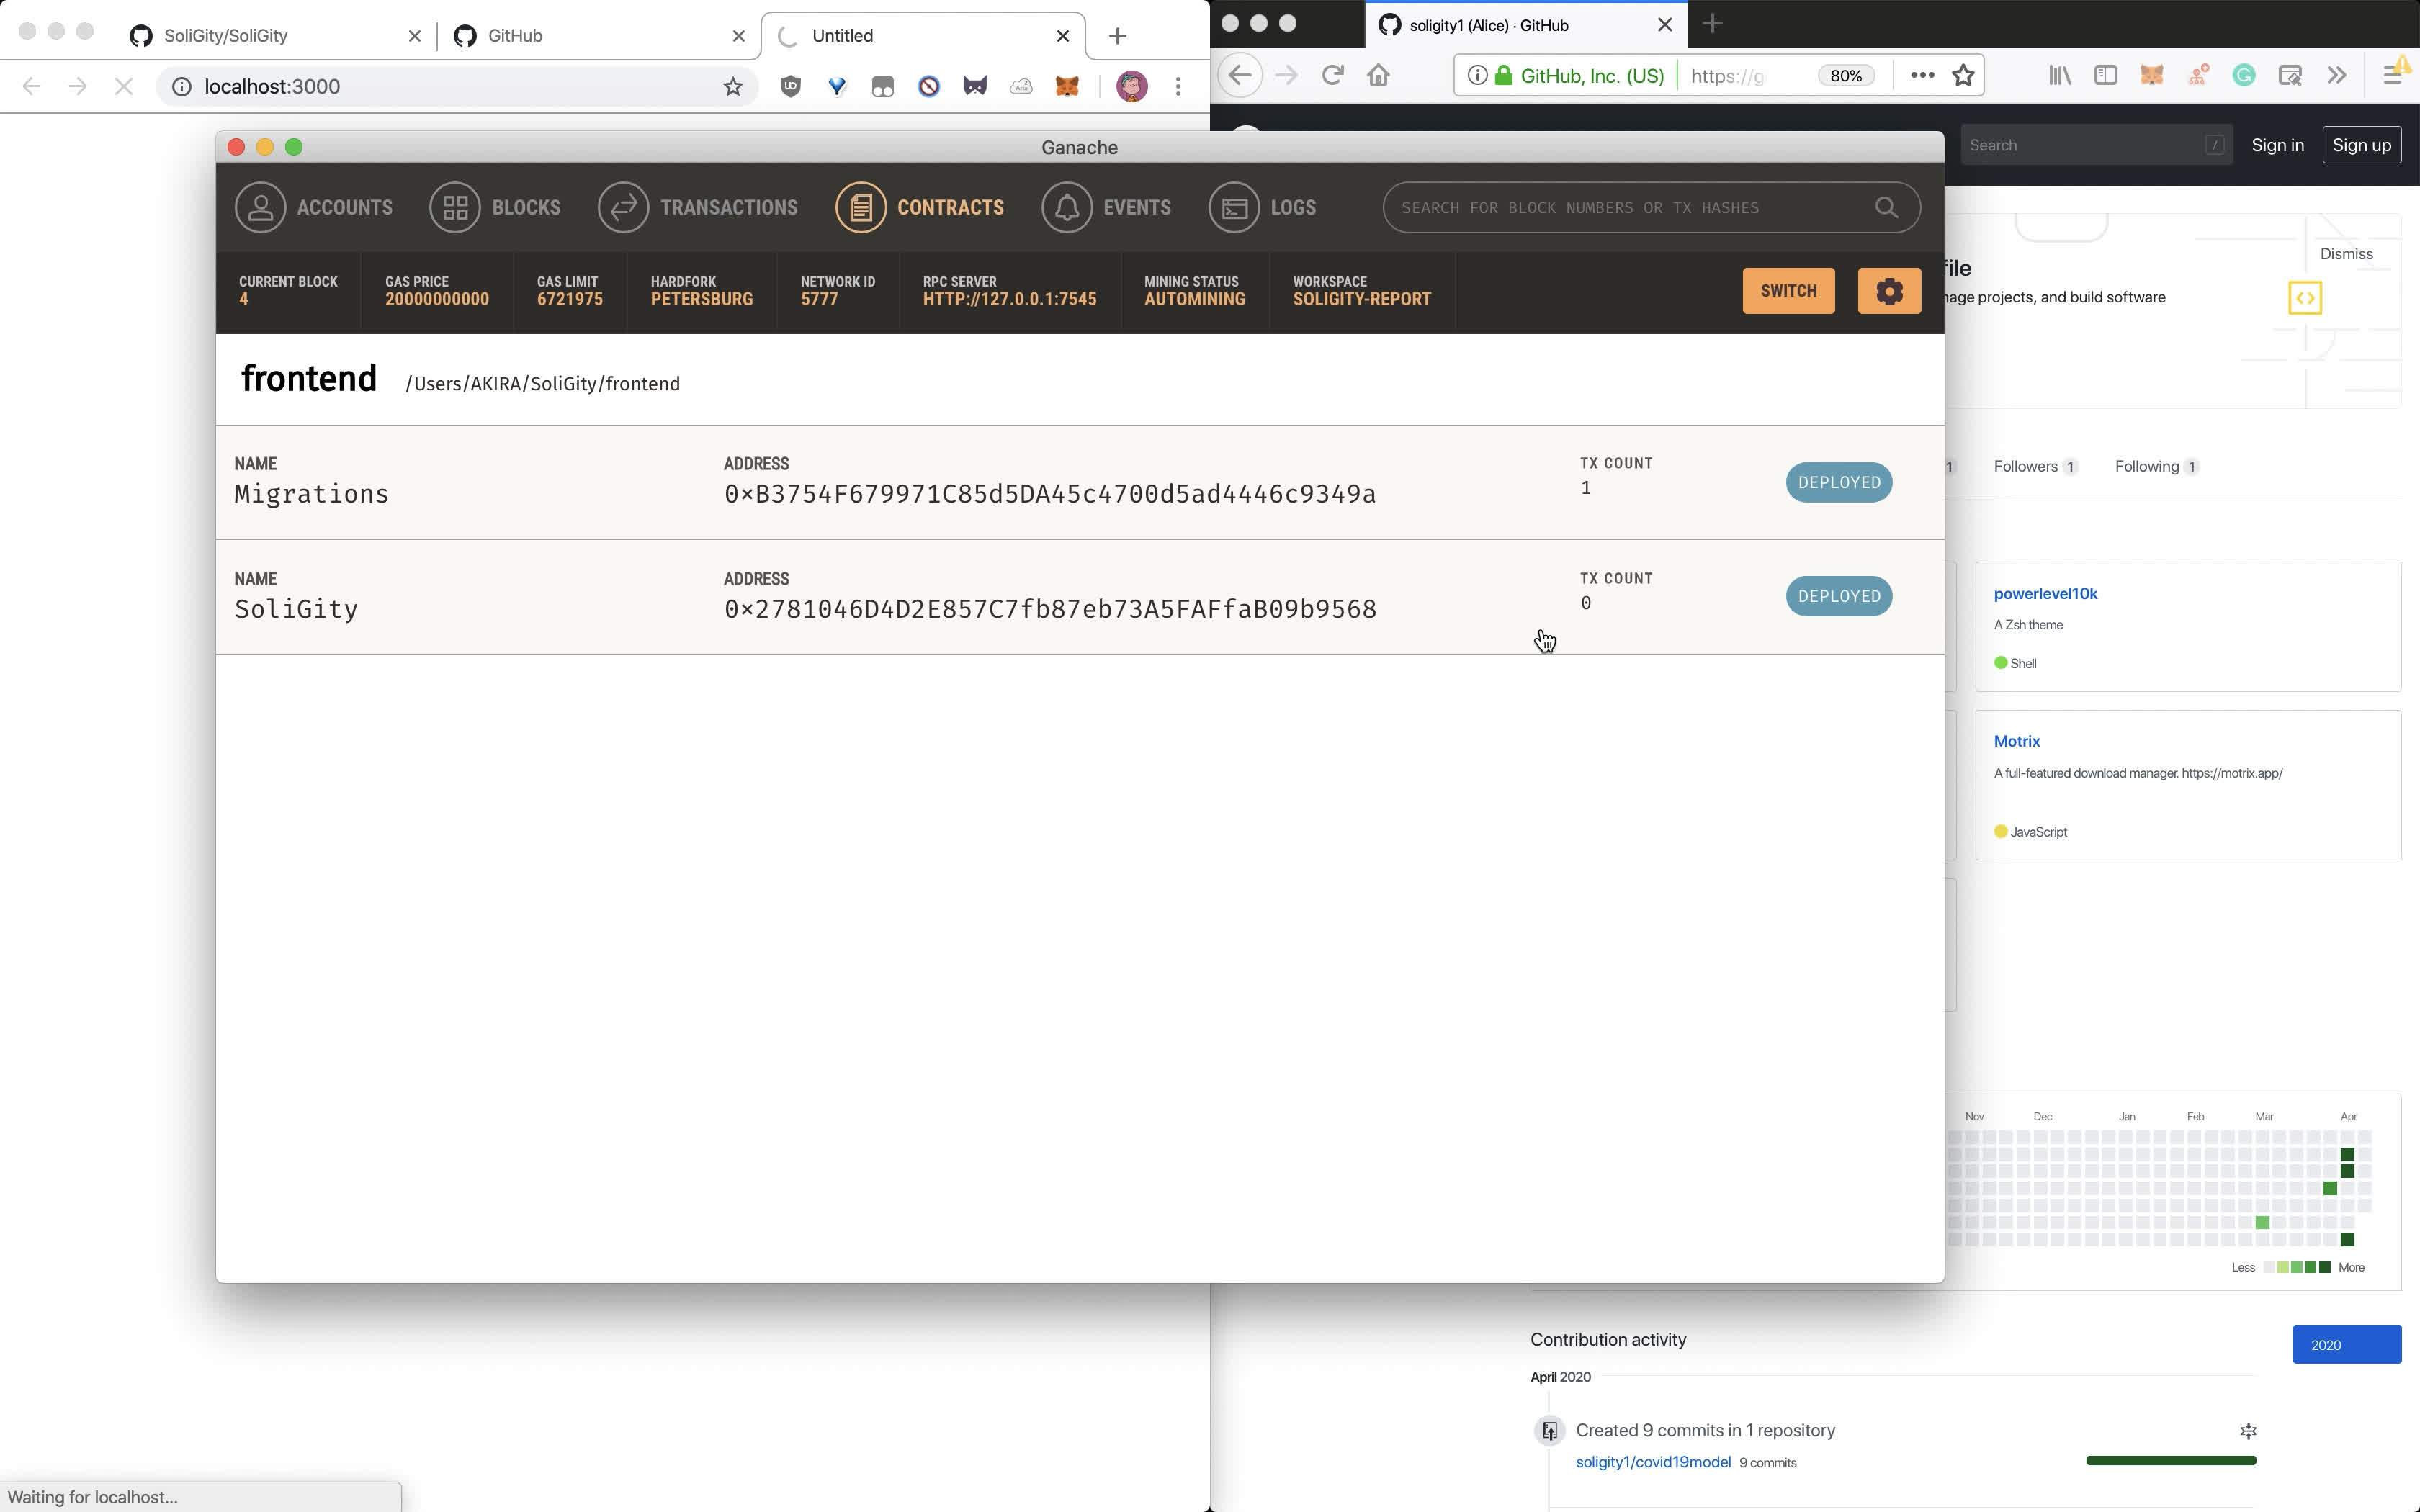
\includegraphics[height=7cm]{graphs/08. ganache_deployed_contract}

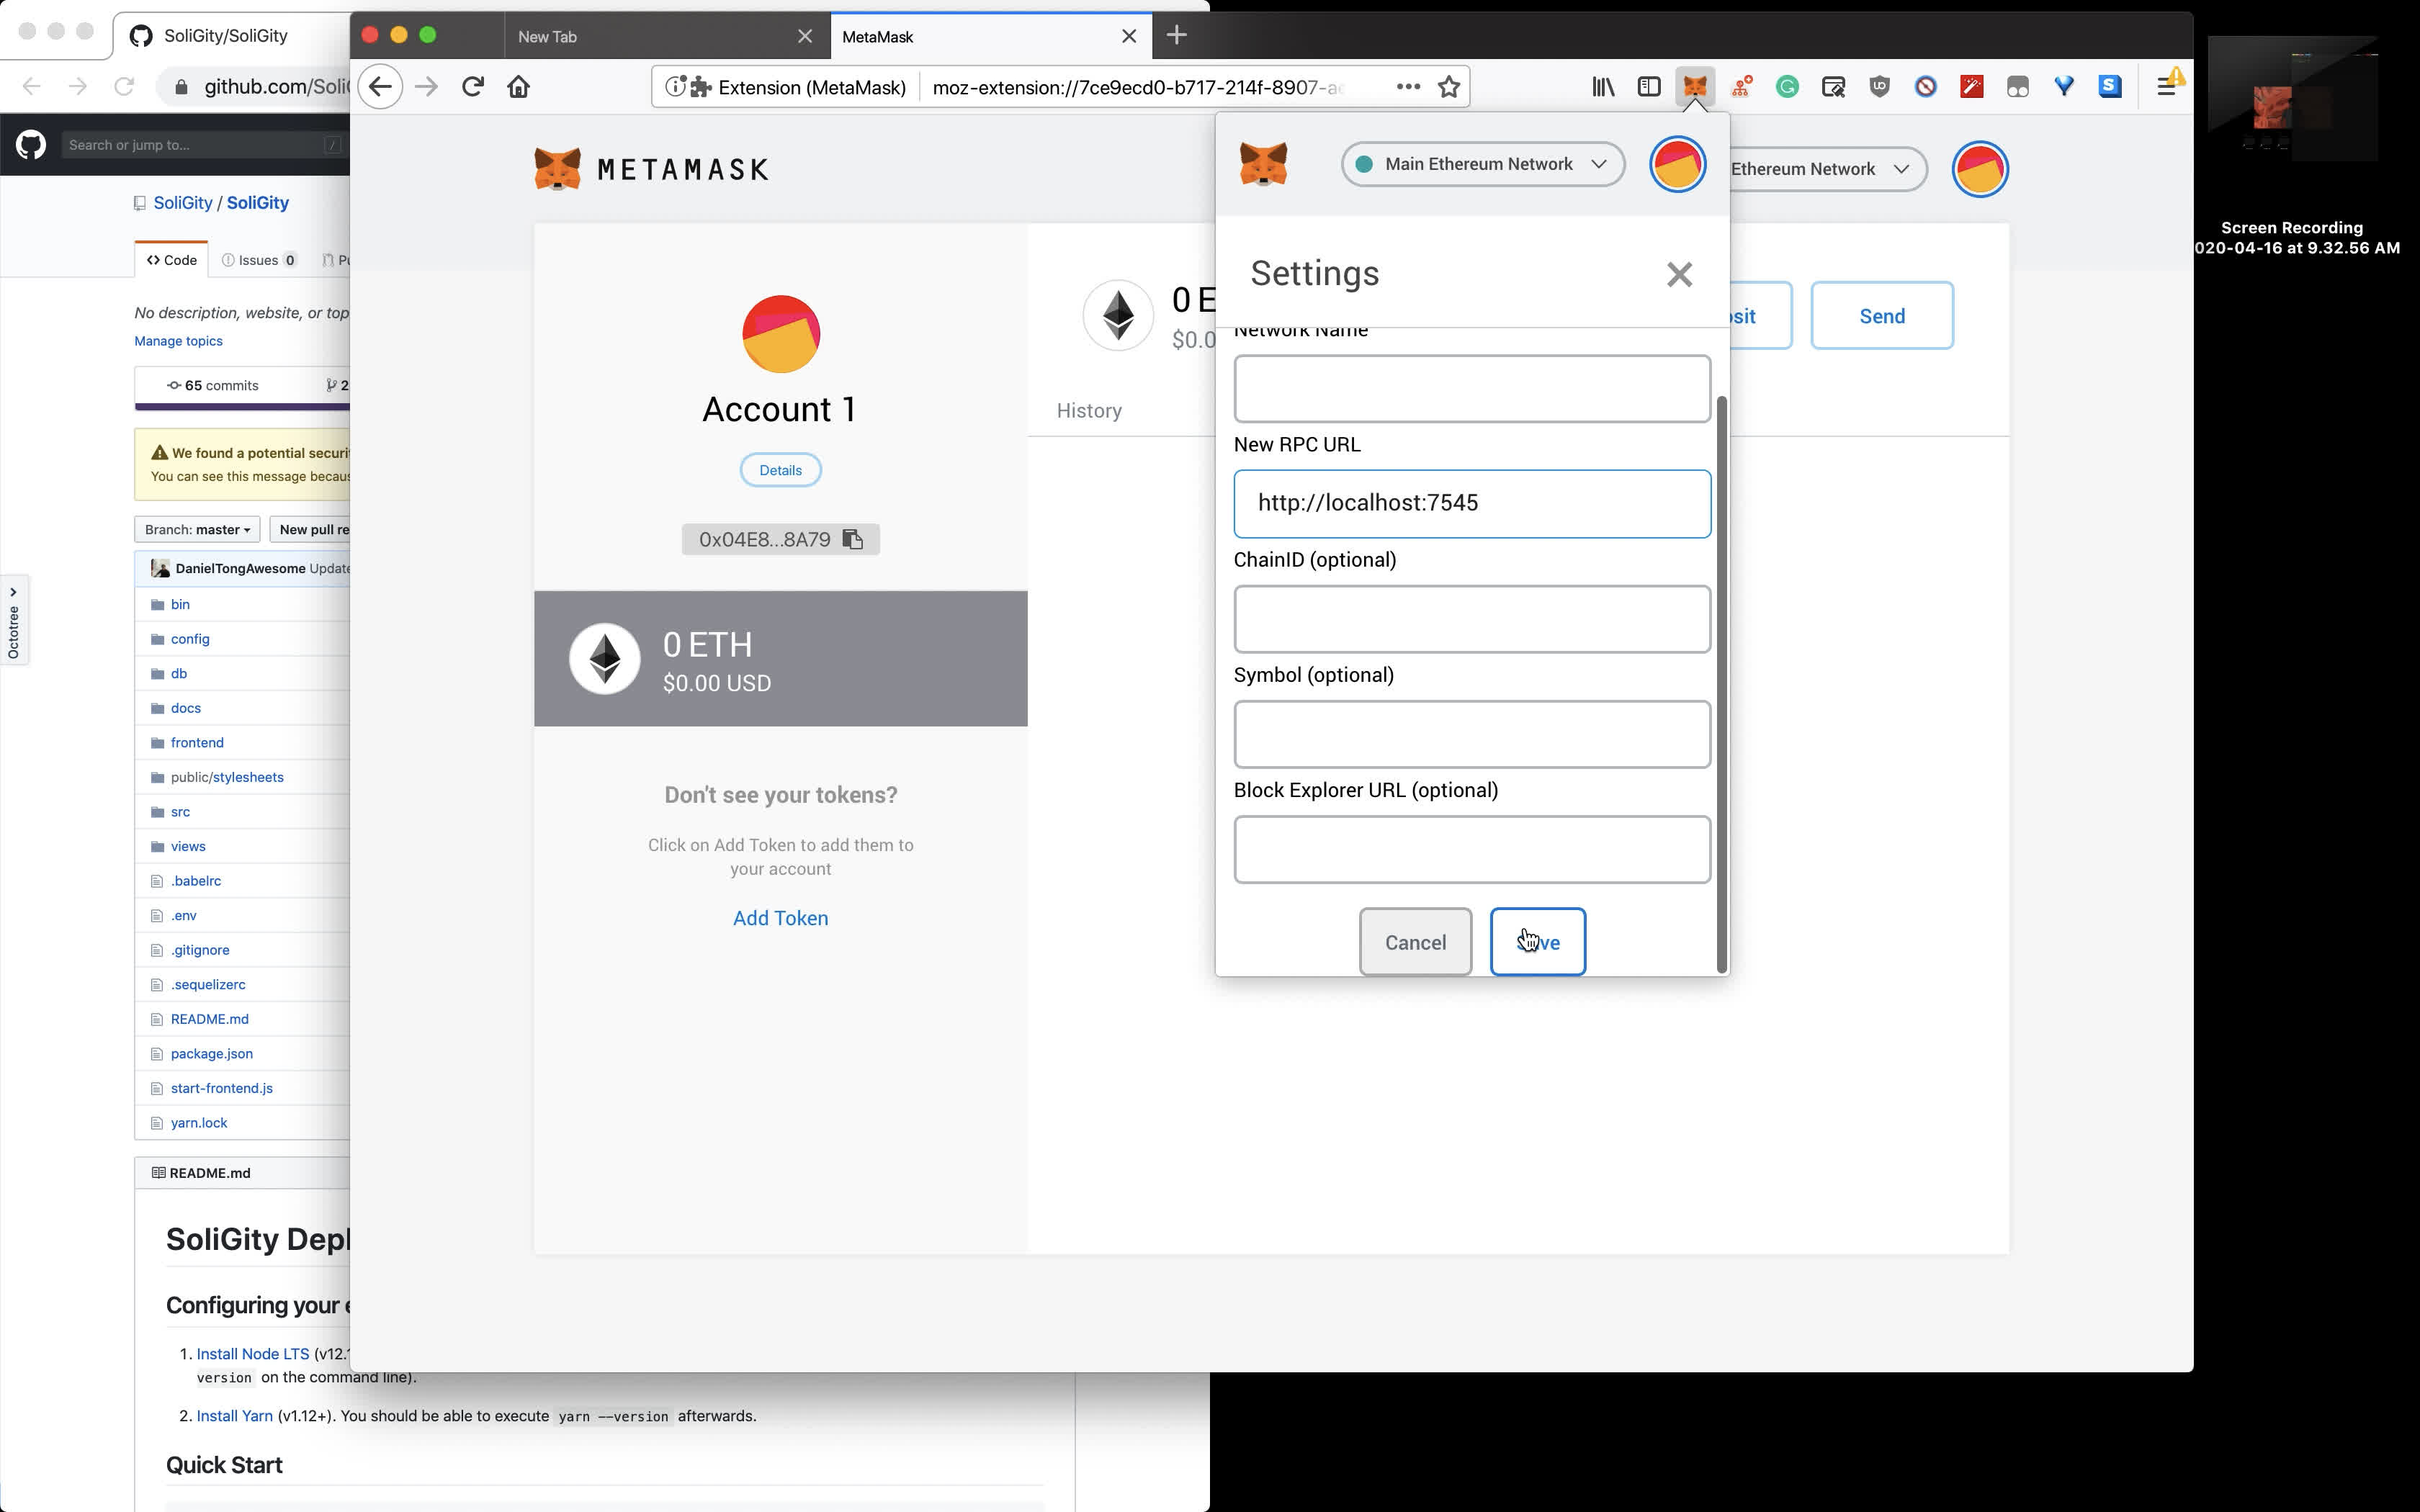
\includegraphics[height=7cm]{graphs/09. metamask_setup_network}

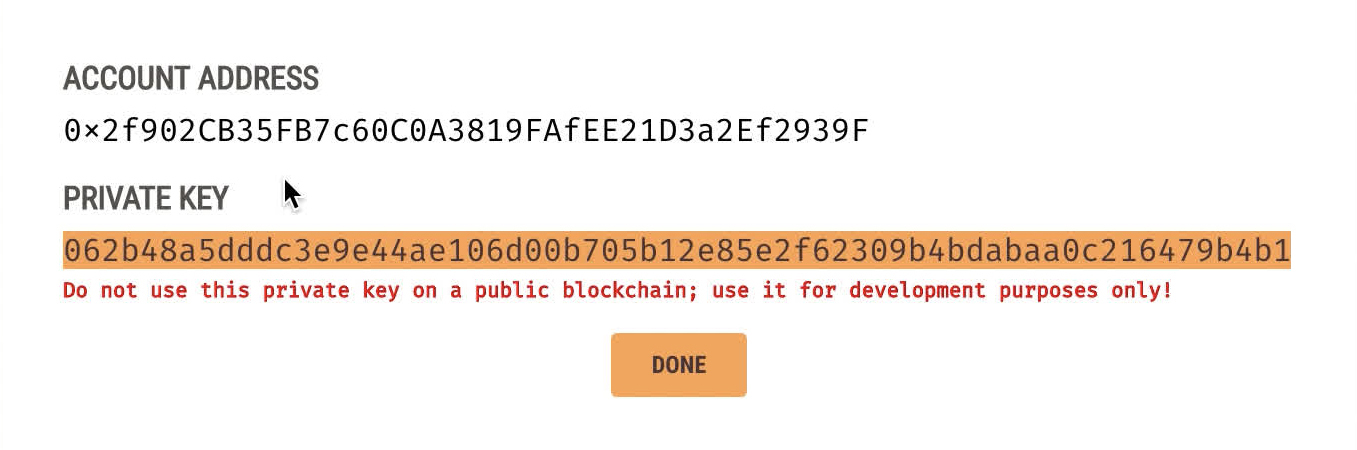
\includegraphics[height=7cm]{graphs/10. metamask_setup_bob}

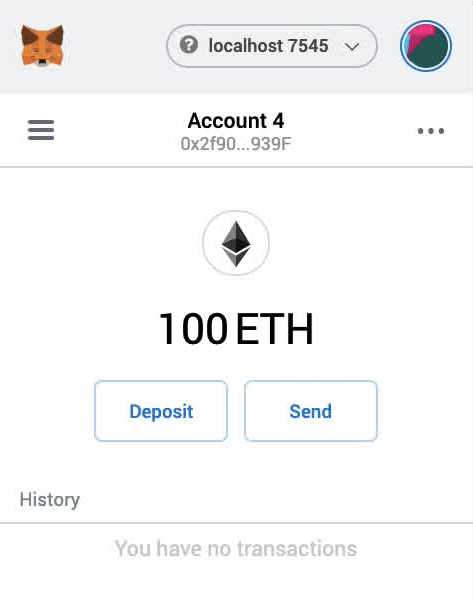
\includegraphics[height=7cm]{graphs/11. metamask_setup_bob}

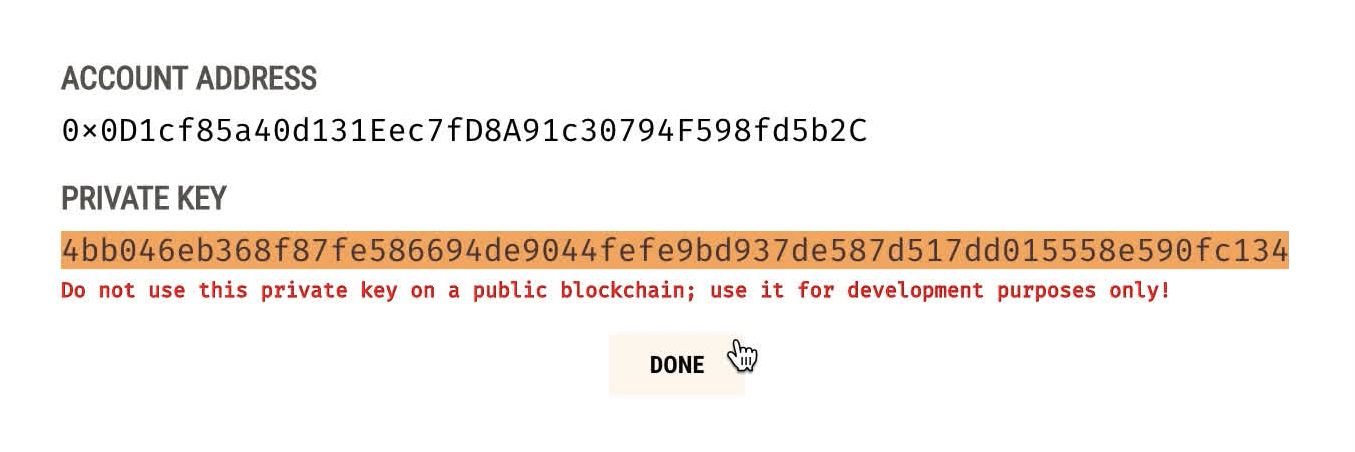
\includegraphics[height=7cm]{graphs/12. metamask_setup_alice}

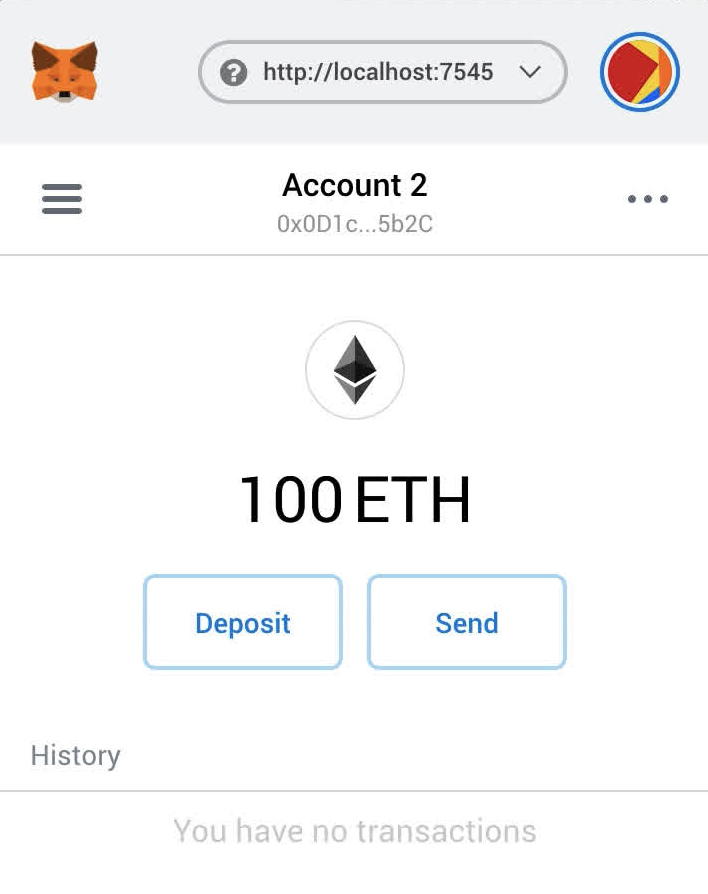
\includegraphics[height=7cm]{graphs/13. metamask_setup_alice}

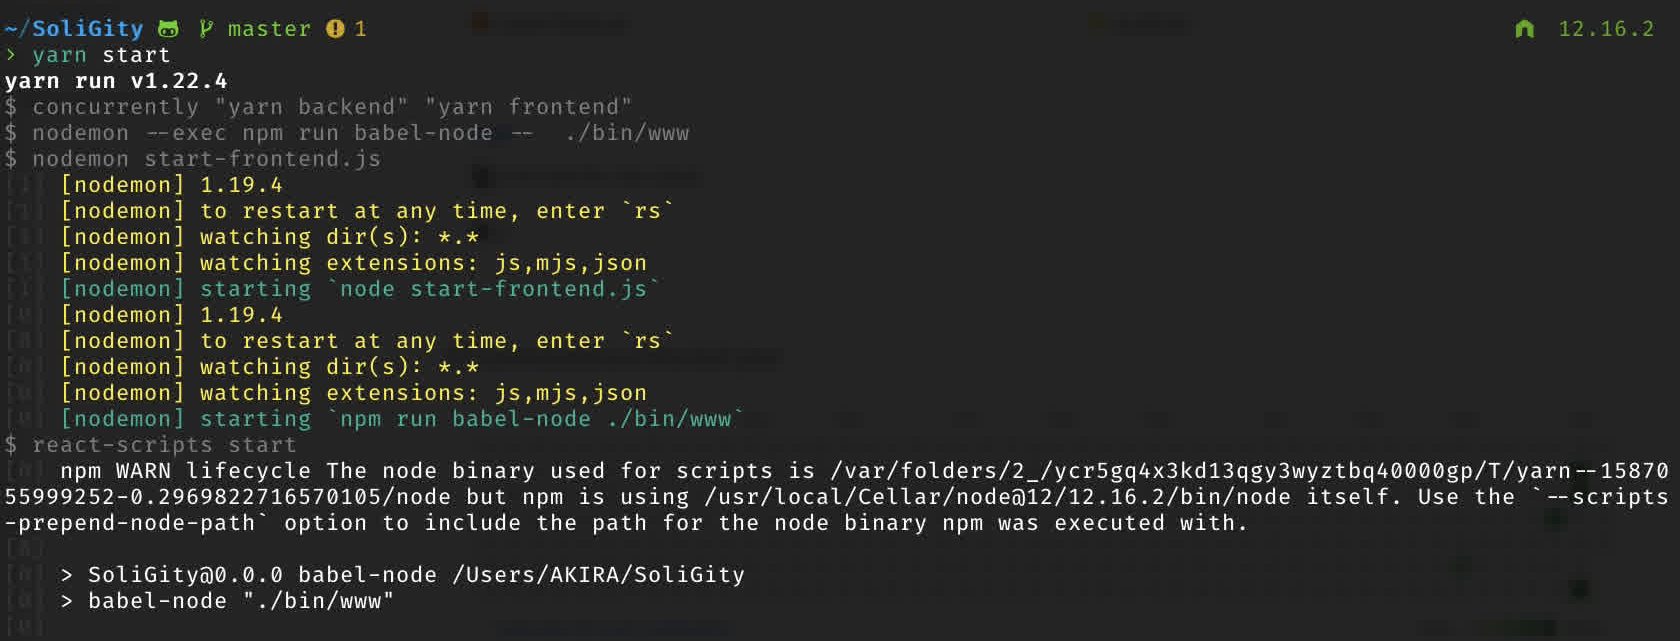
\includegraphics[height=7cm]{graphs/14. yarn_start}

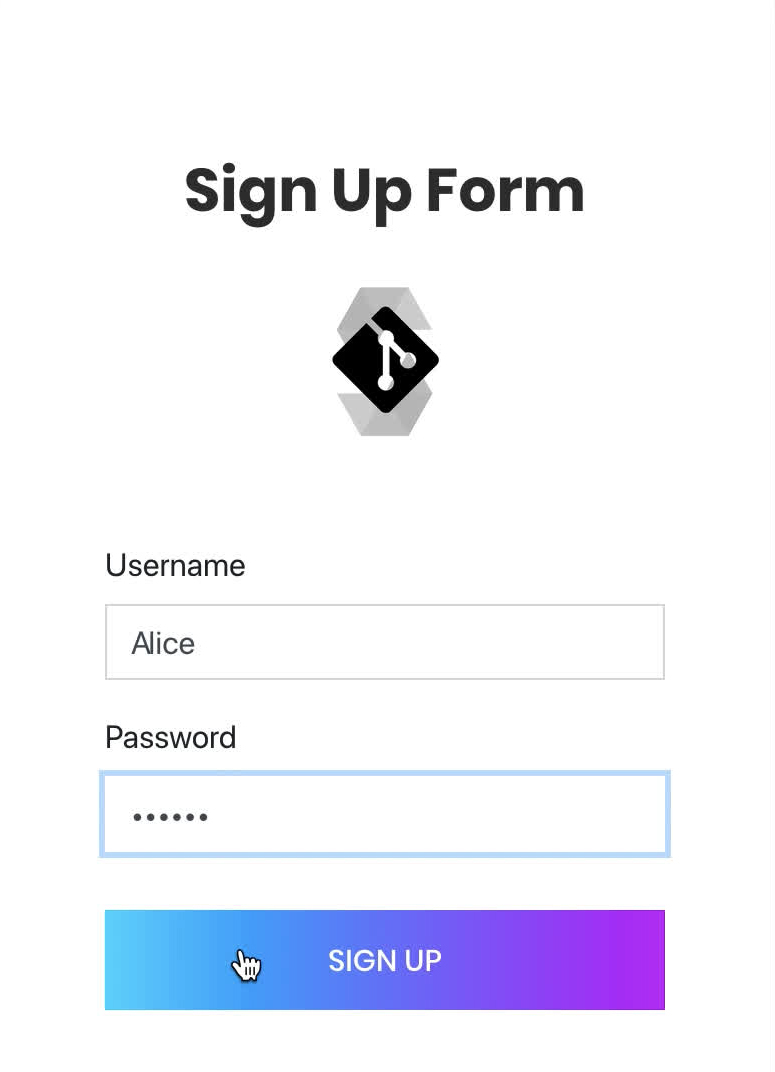
\includegraphics[height=7cm]{graphs/15. alice_sign_up}

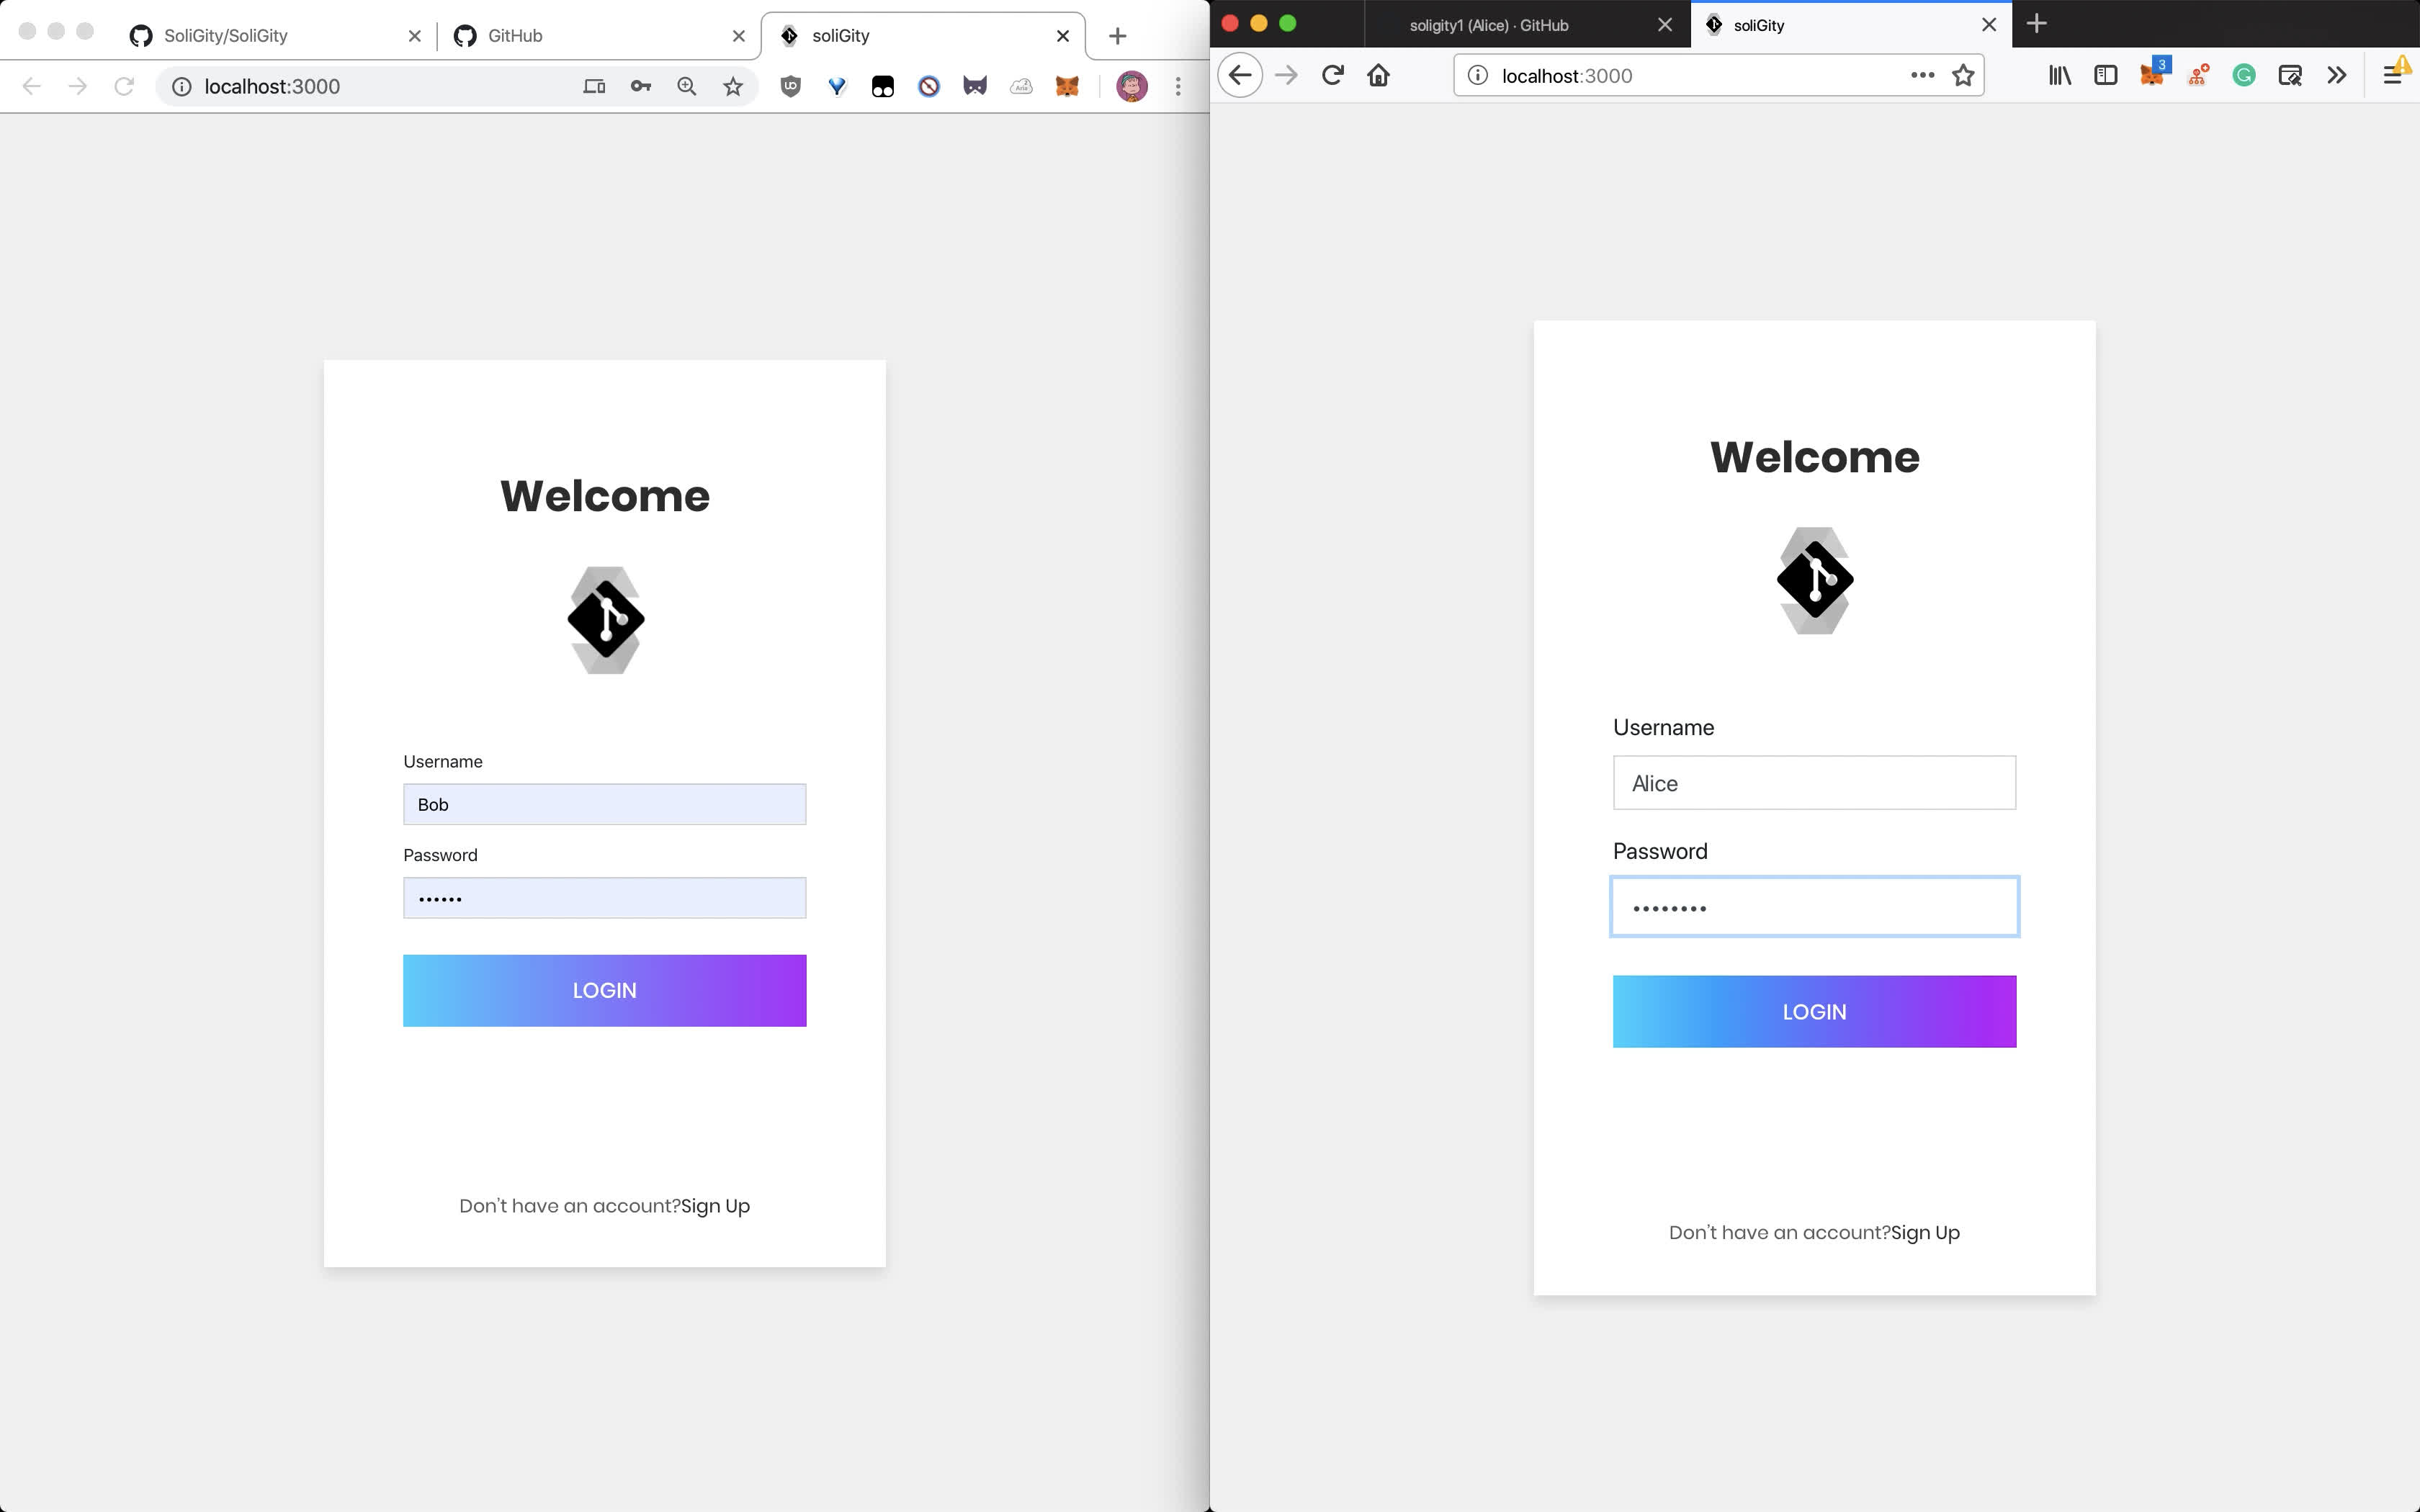
\includegraphics[height=7cm]{graphs/16. alice_login}

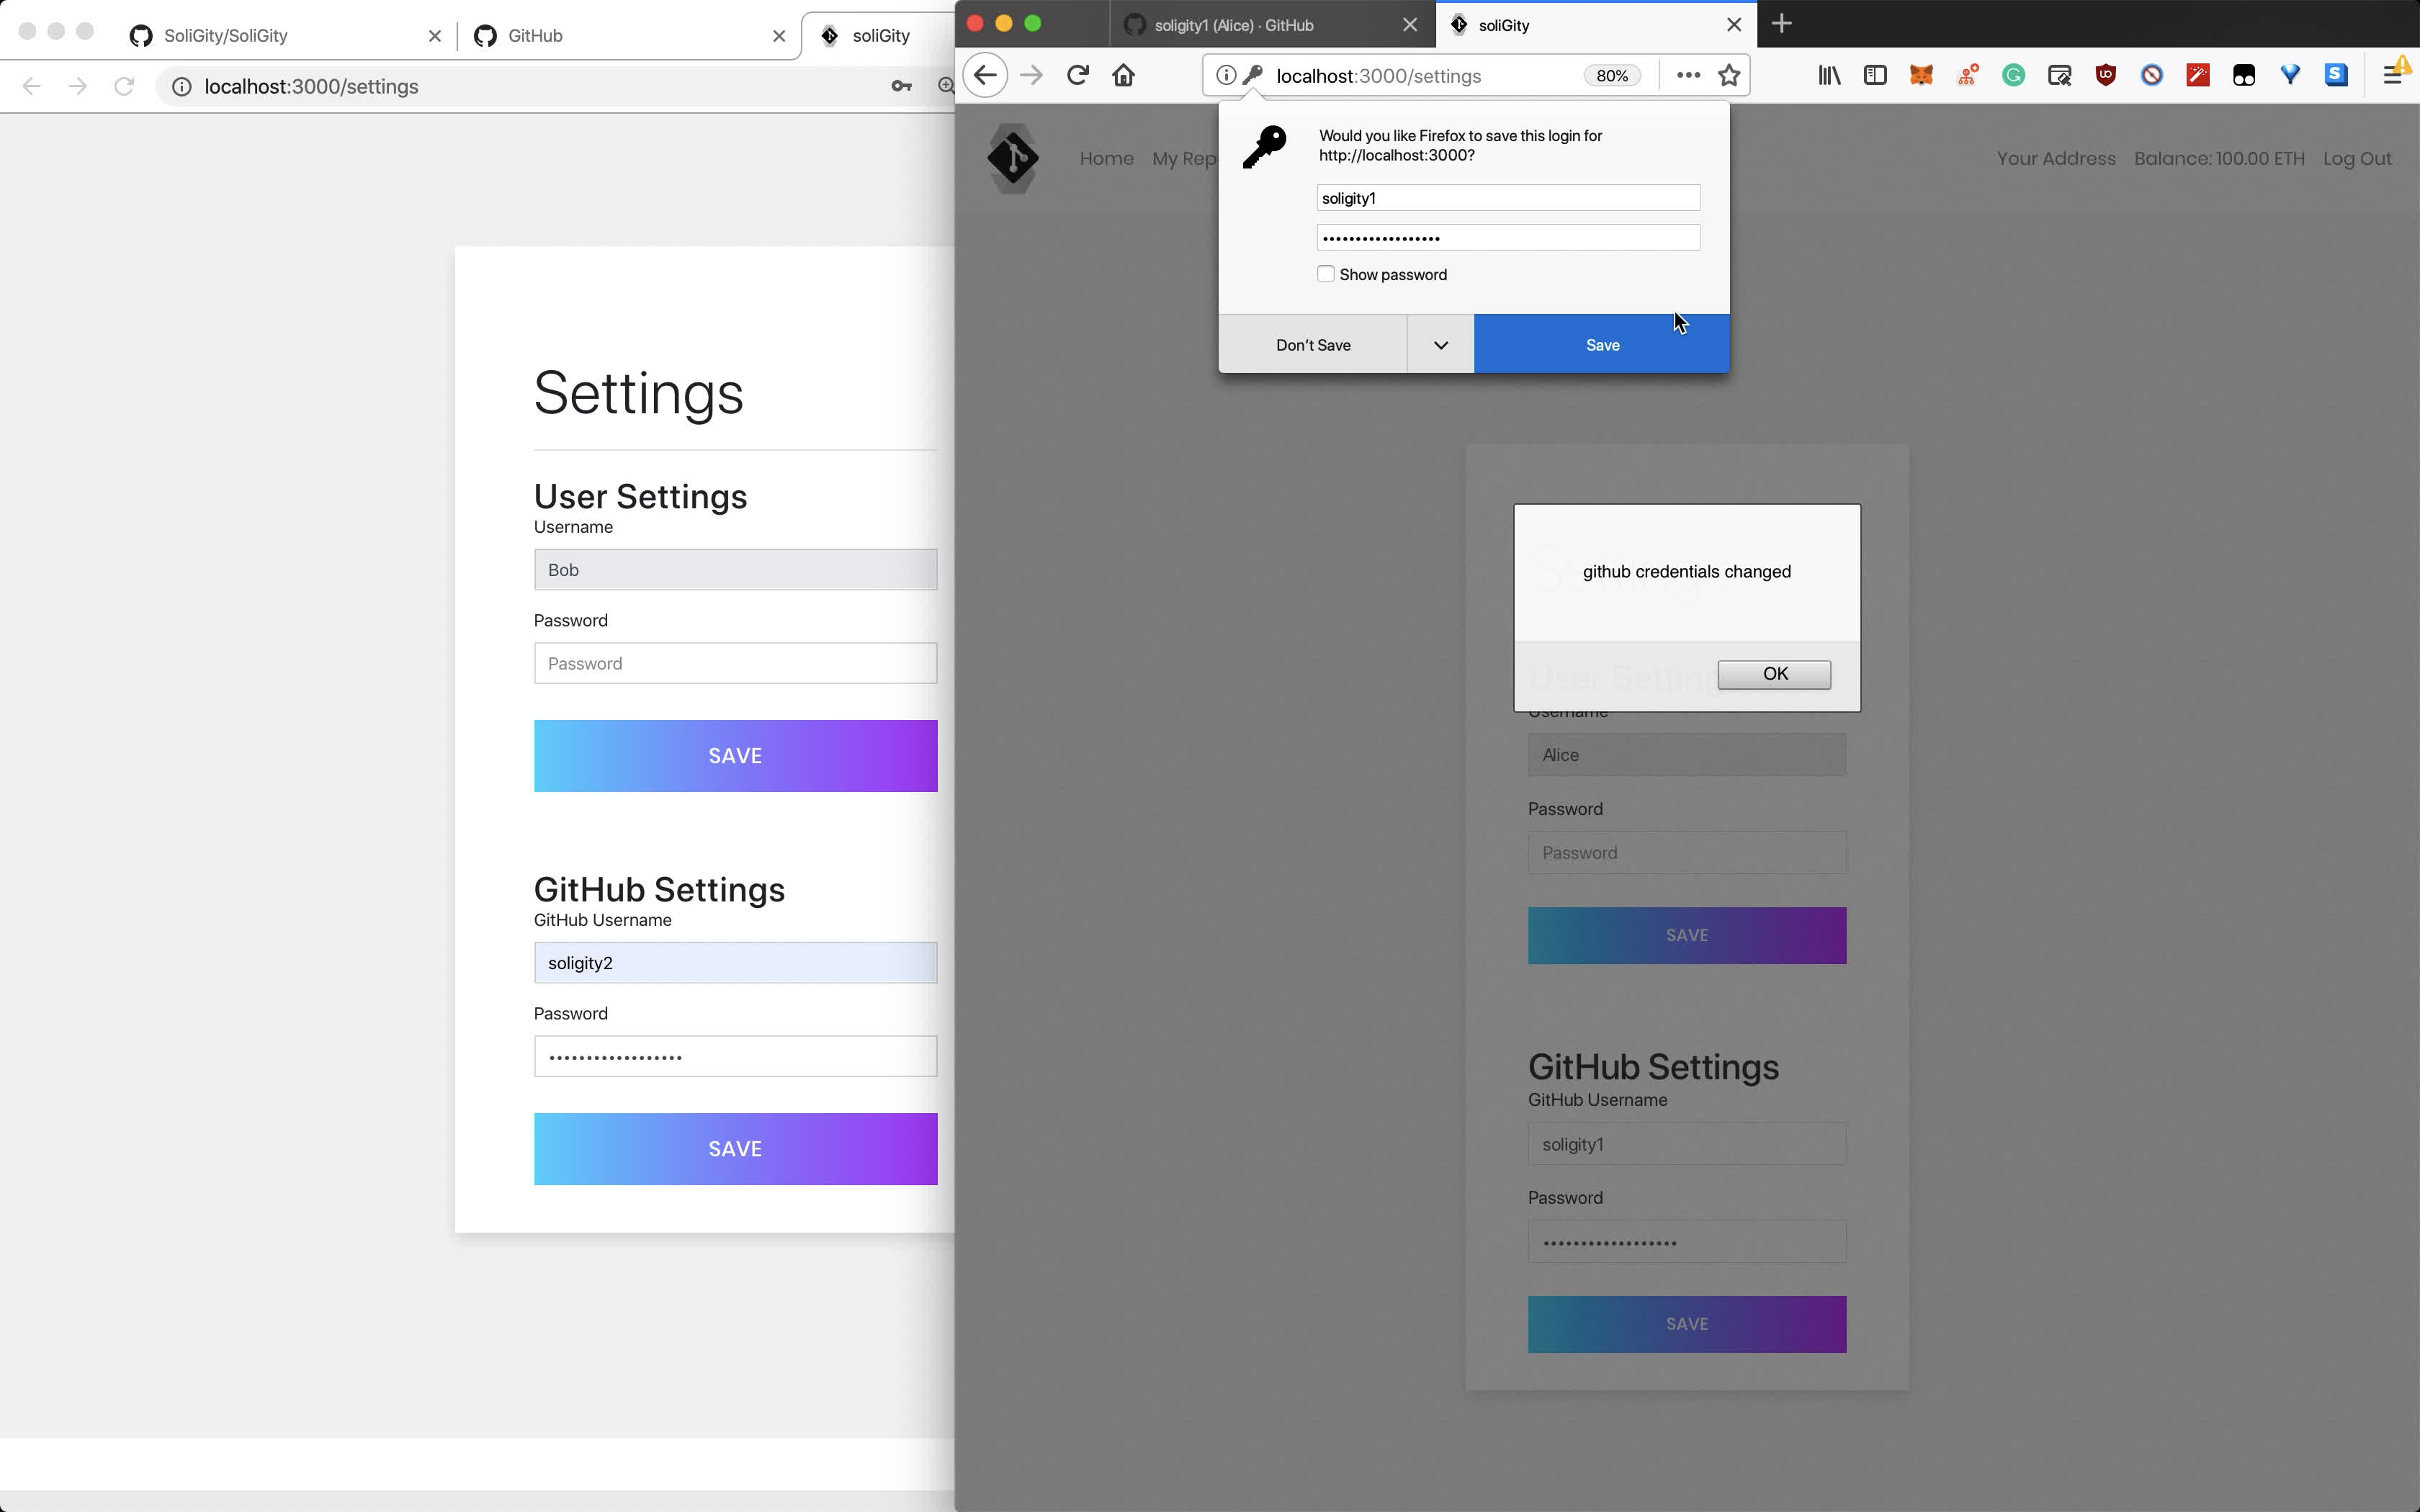
\includegraphics[height=7cm]{graphs/17. alice_gitub_setup}

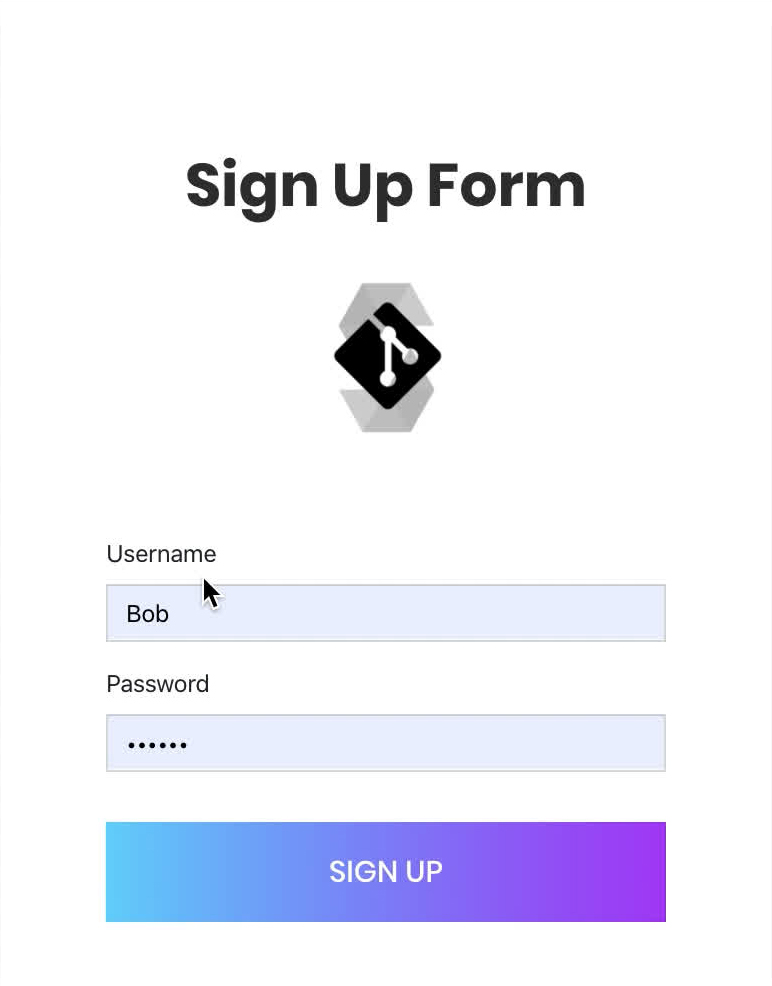
\includegraphics[height=7cm]{graphs/18. bob_sign_up}

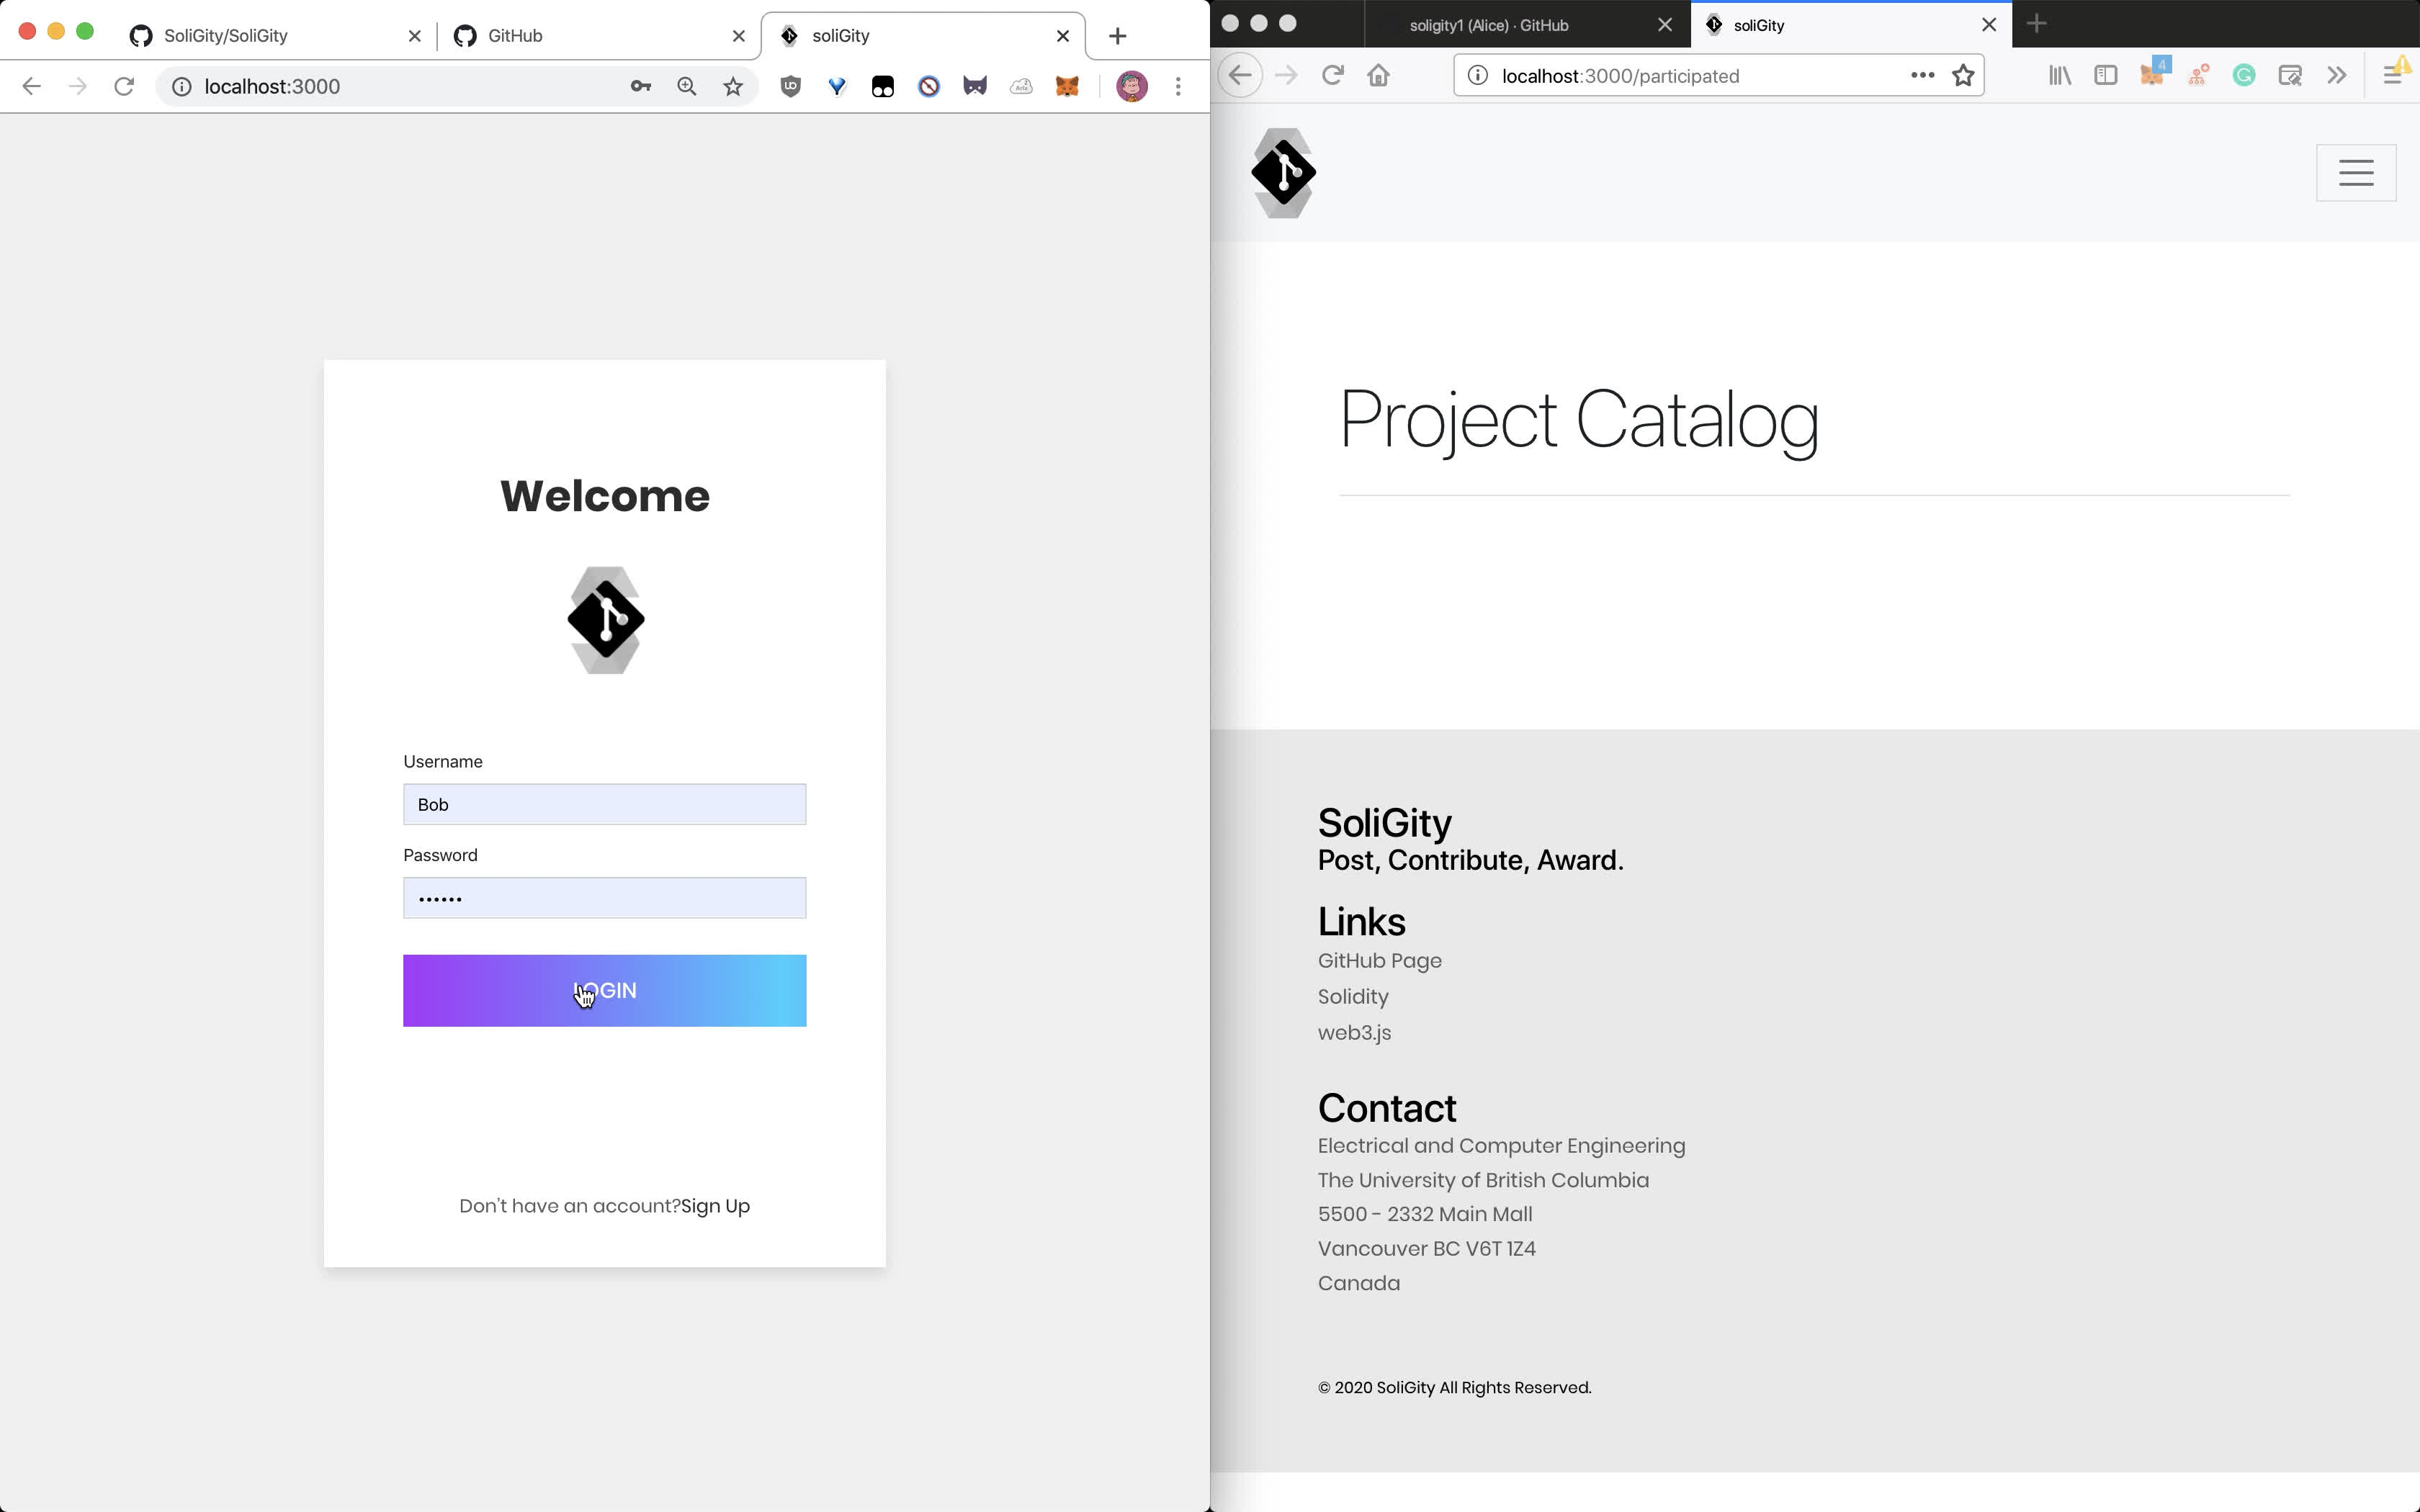
\includegraphics[height=7cm]{graphs/19. bob_login}

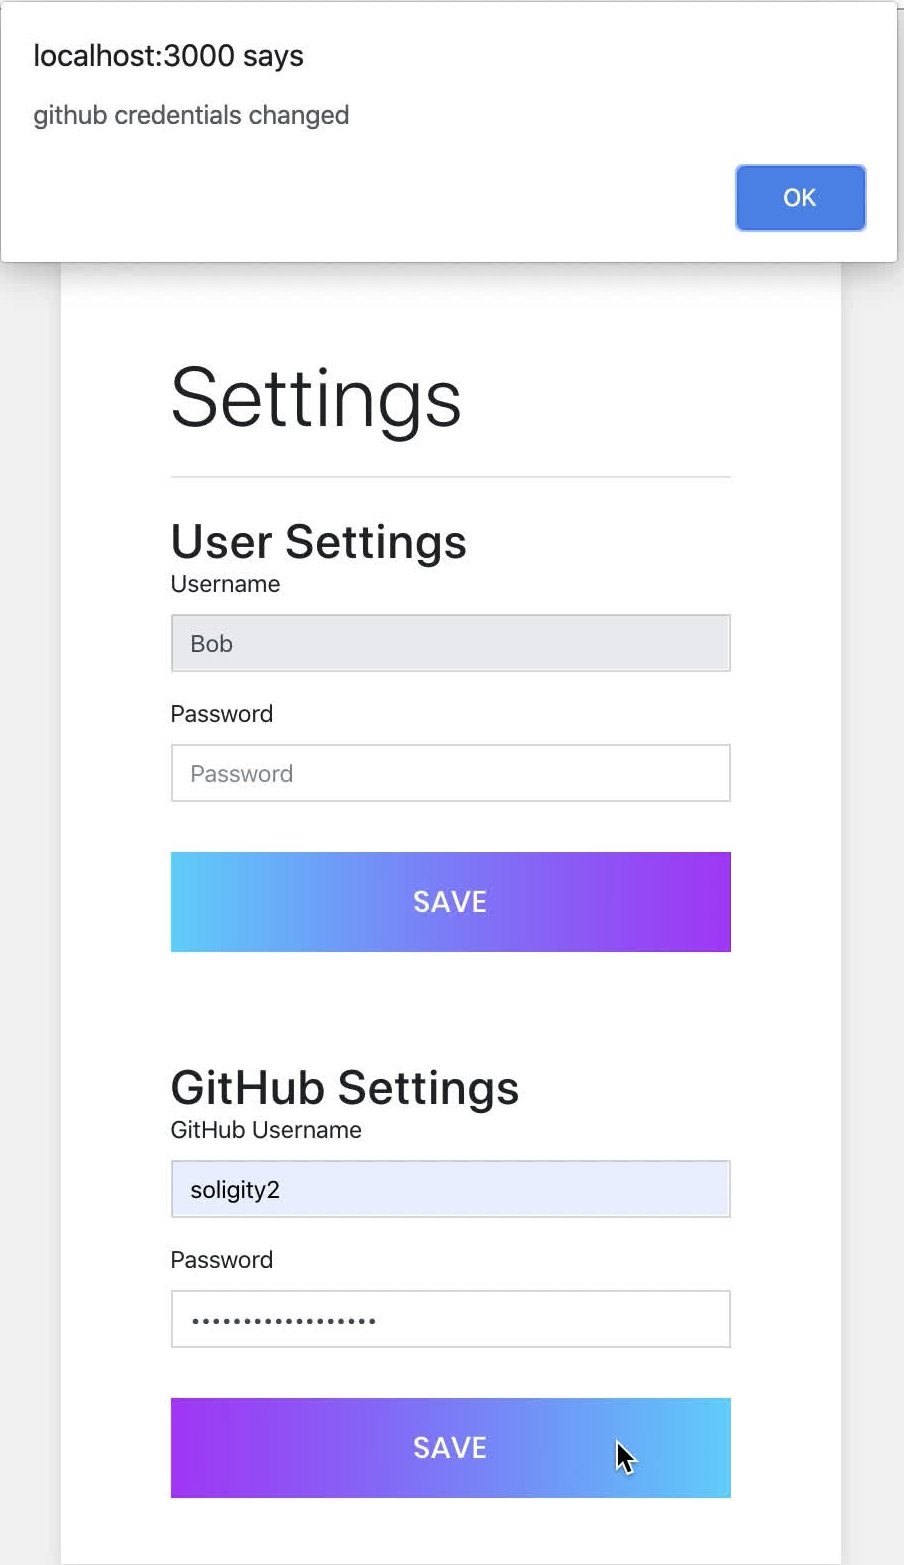
\includegraphics[height=7cm]{graphs/20. bob_gitub_setup}

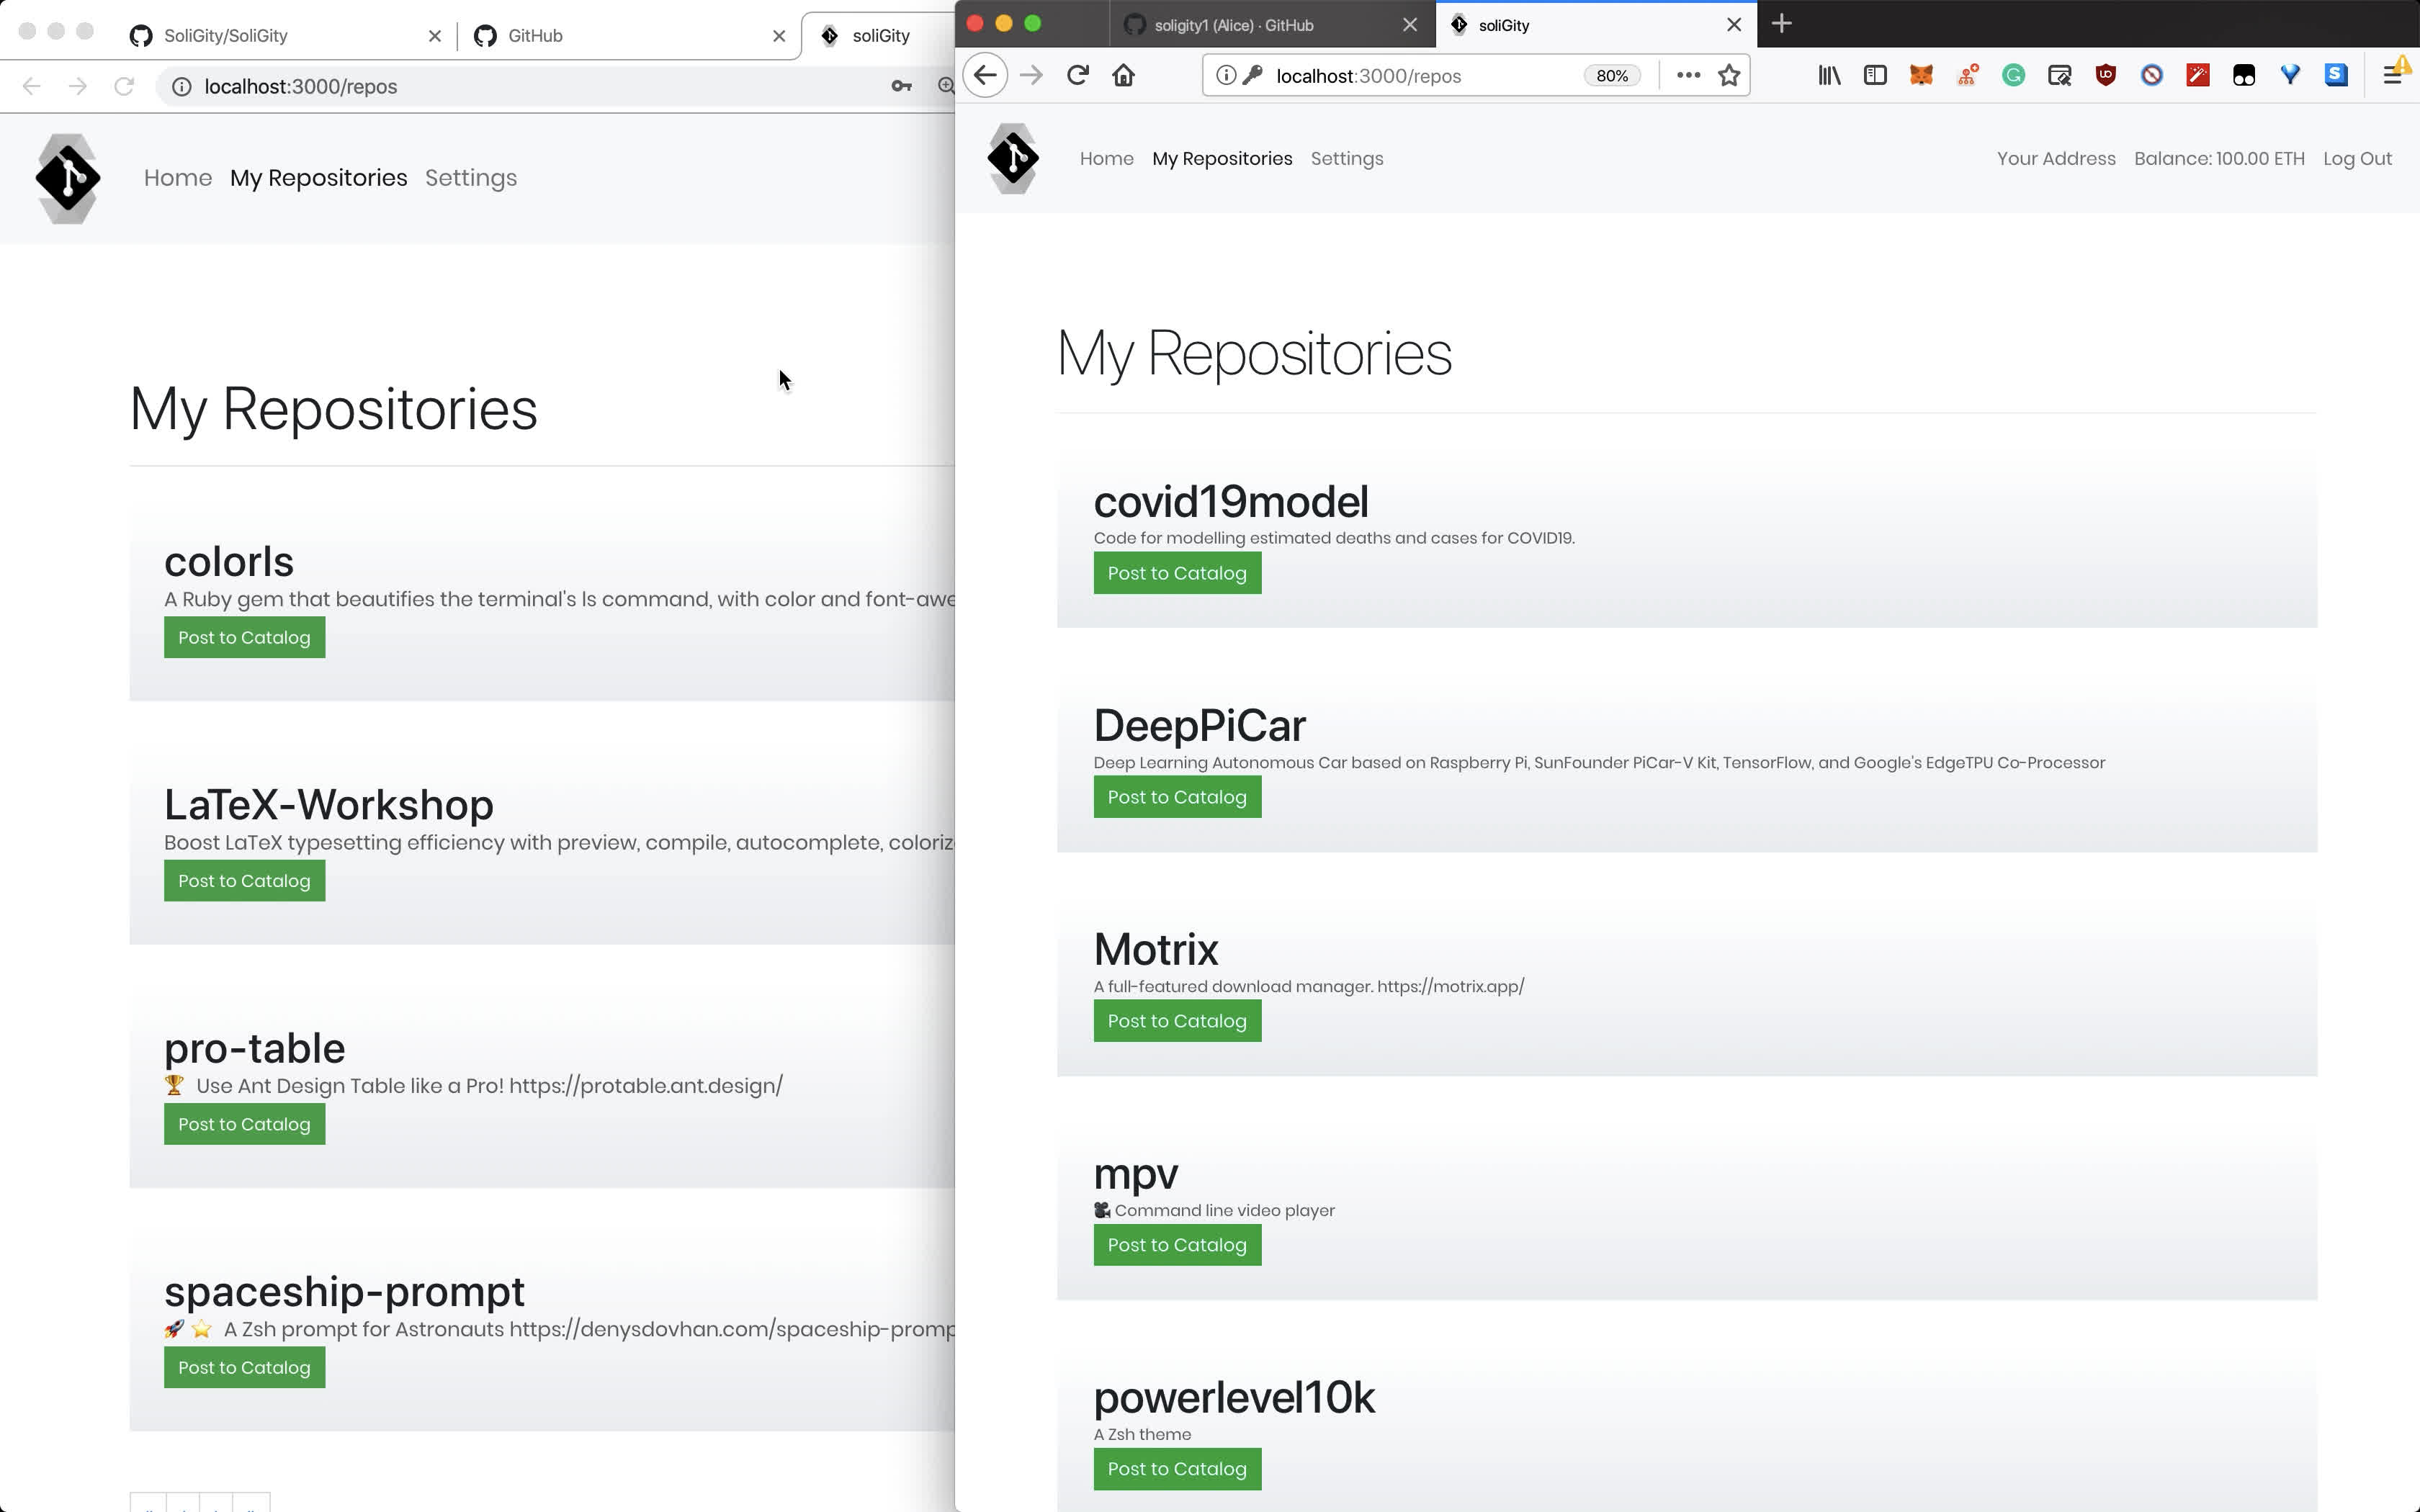
\includegraphics[height=7cm]{graphs/21. alice_bob_repos}


\includegraphics[height=7cm]{graphs/22. empty_project_catalog}

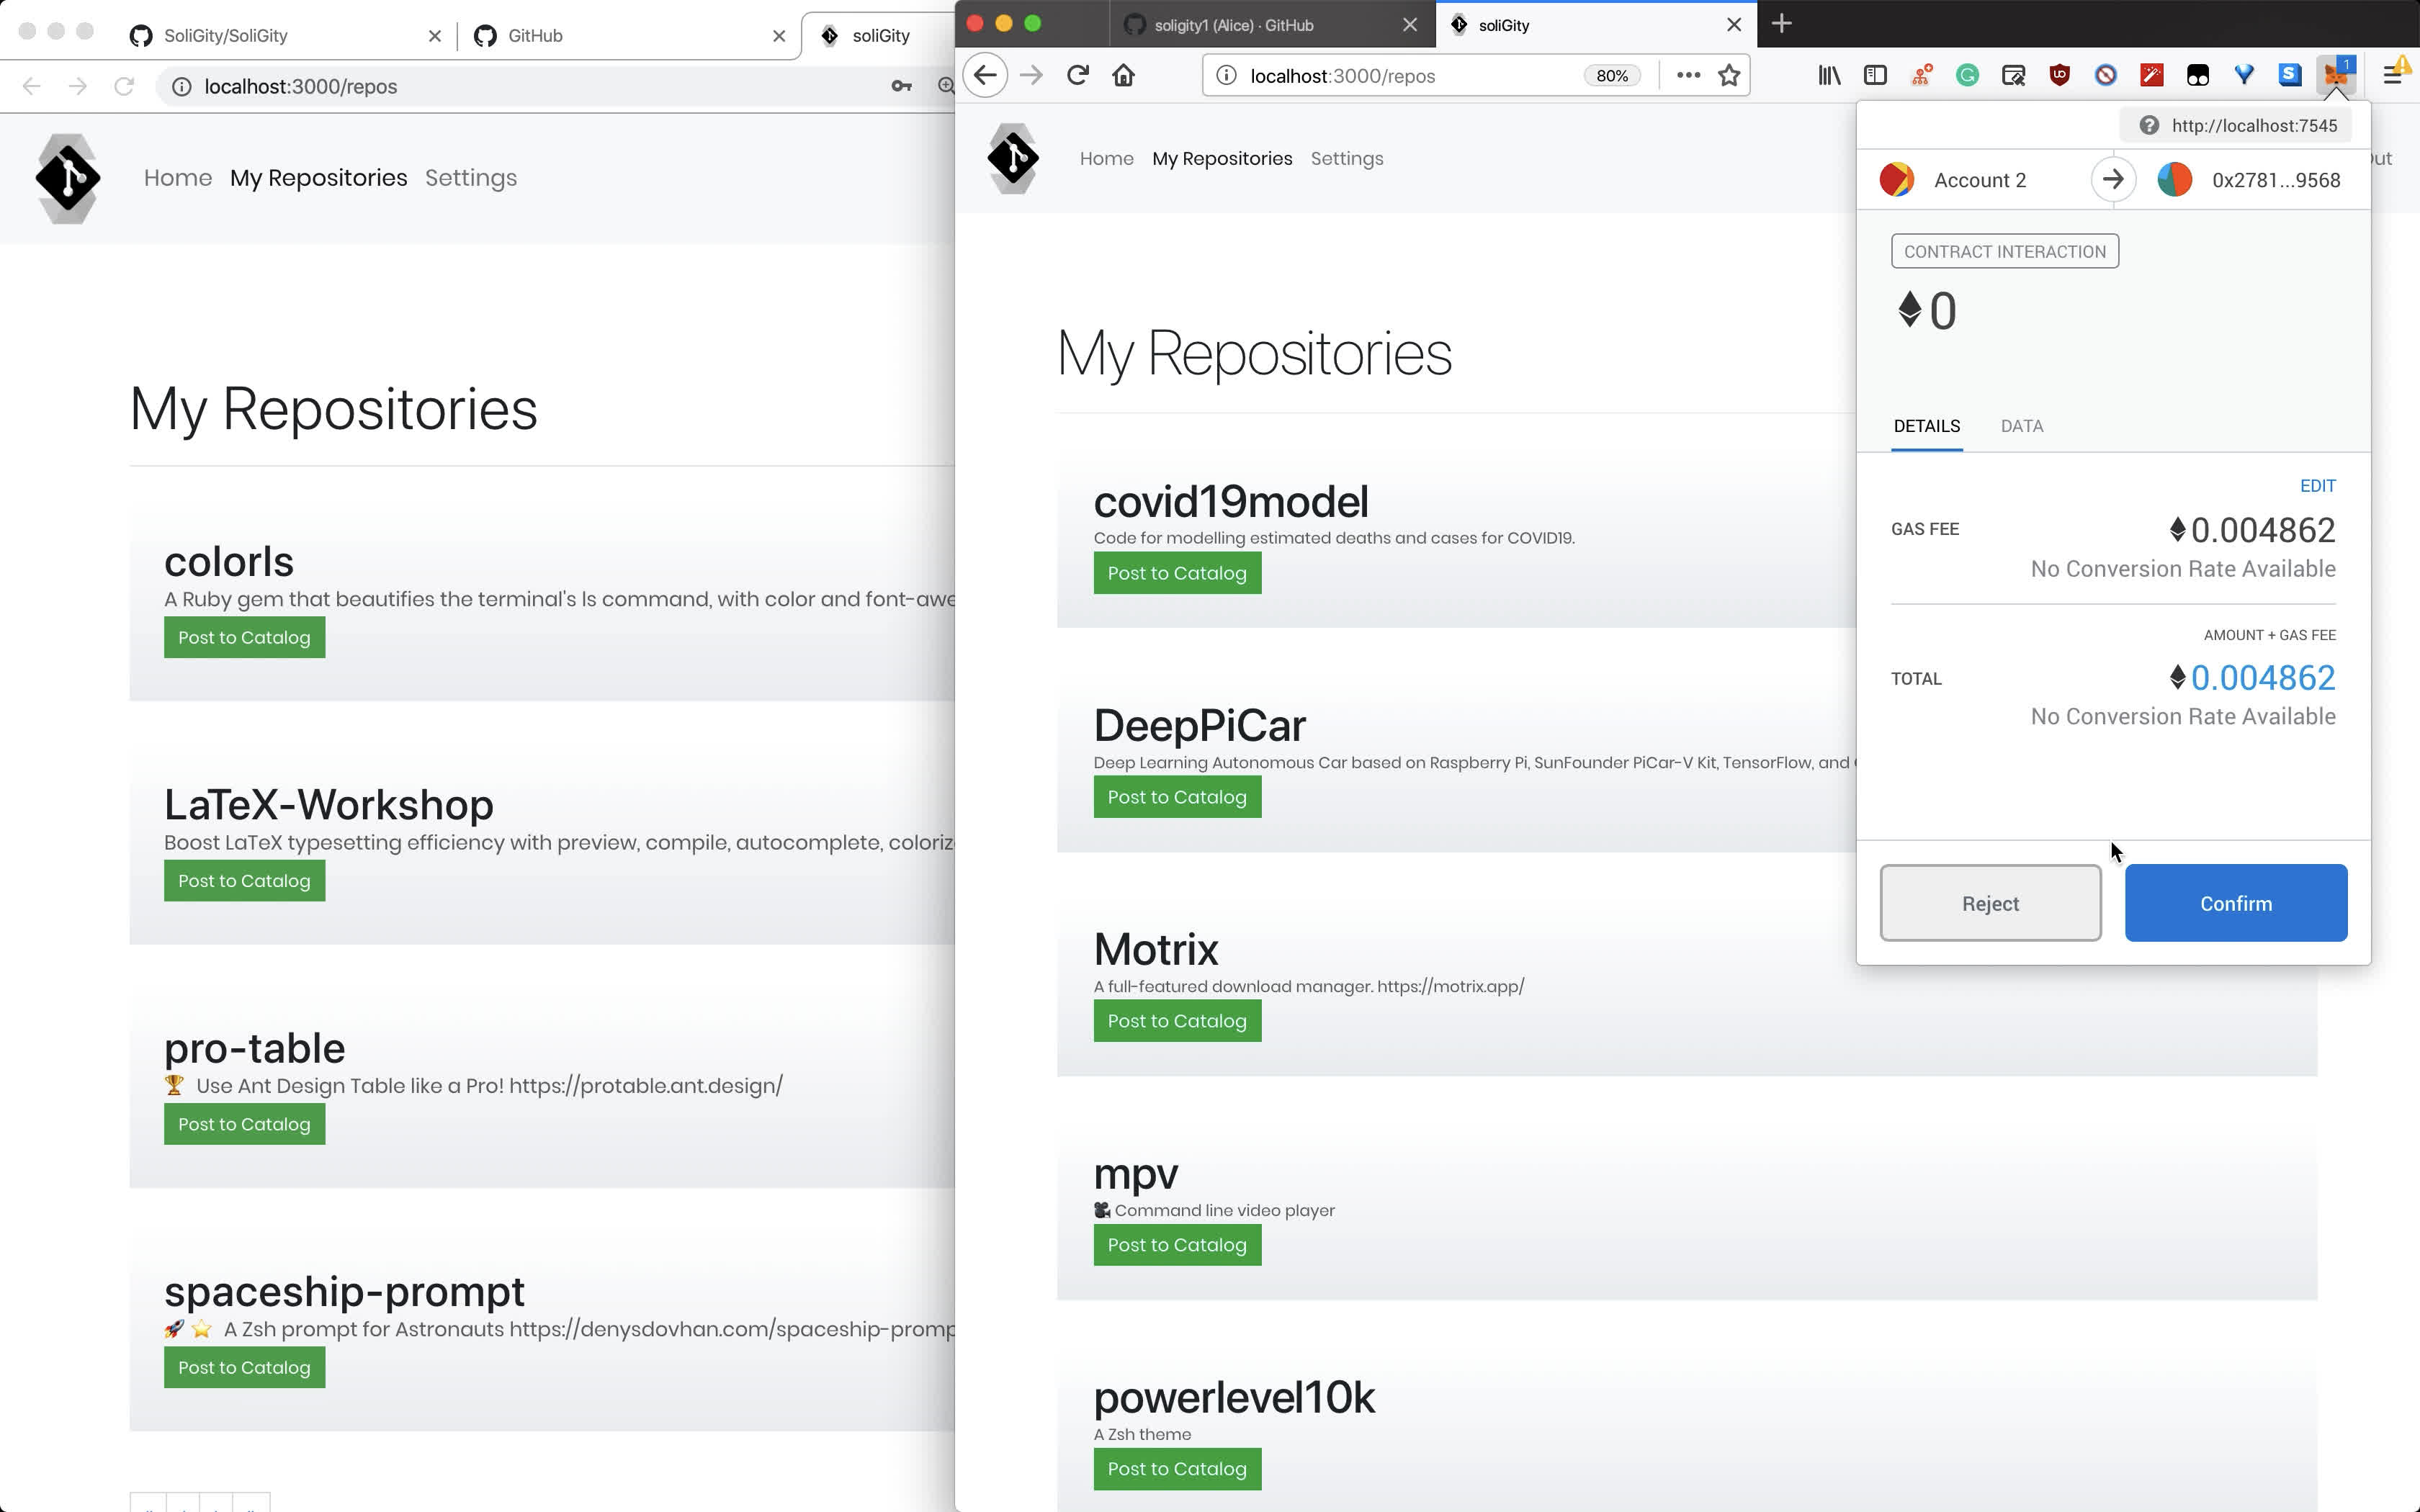
\includegraphics[height=7cm]{graphs/23. alice_post_to_catalog_1}

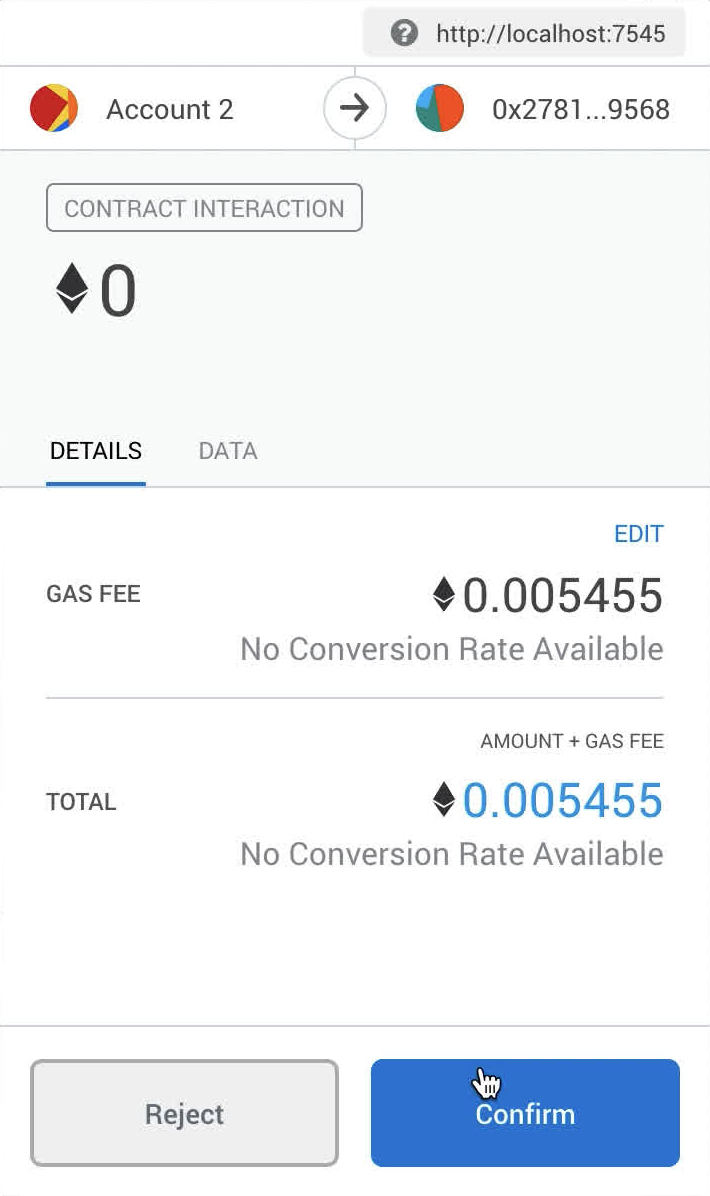
\includegraphics[height=7cm]{graphs/24. alice_post_to_catalog_2}

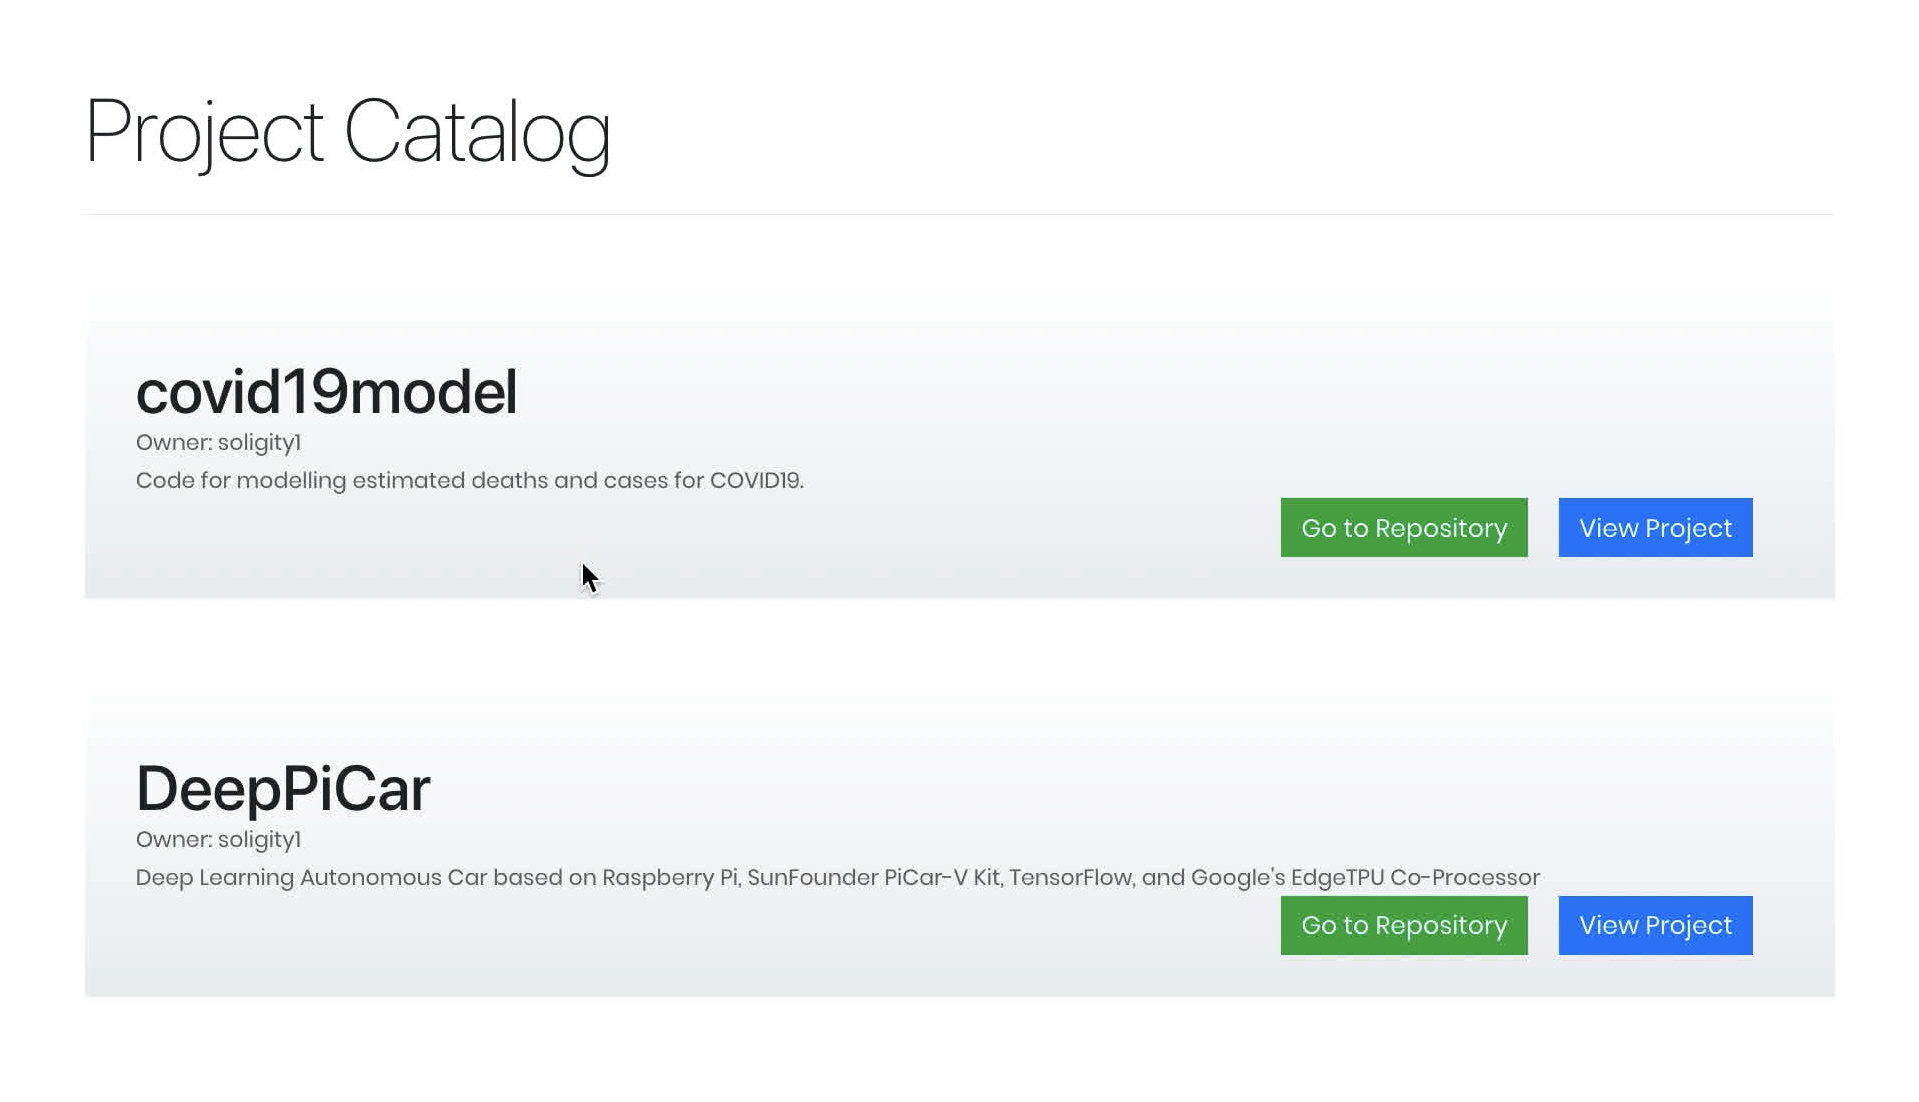
\includegraphics[height=7cm]{graphs/25. added_project_catalog}

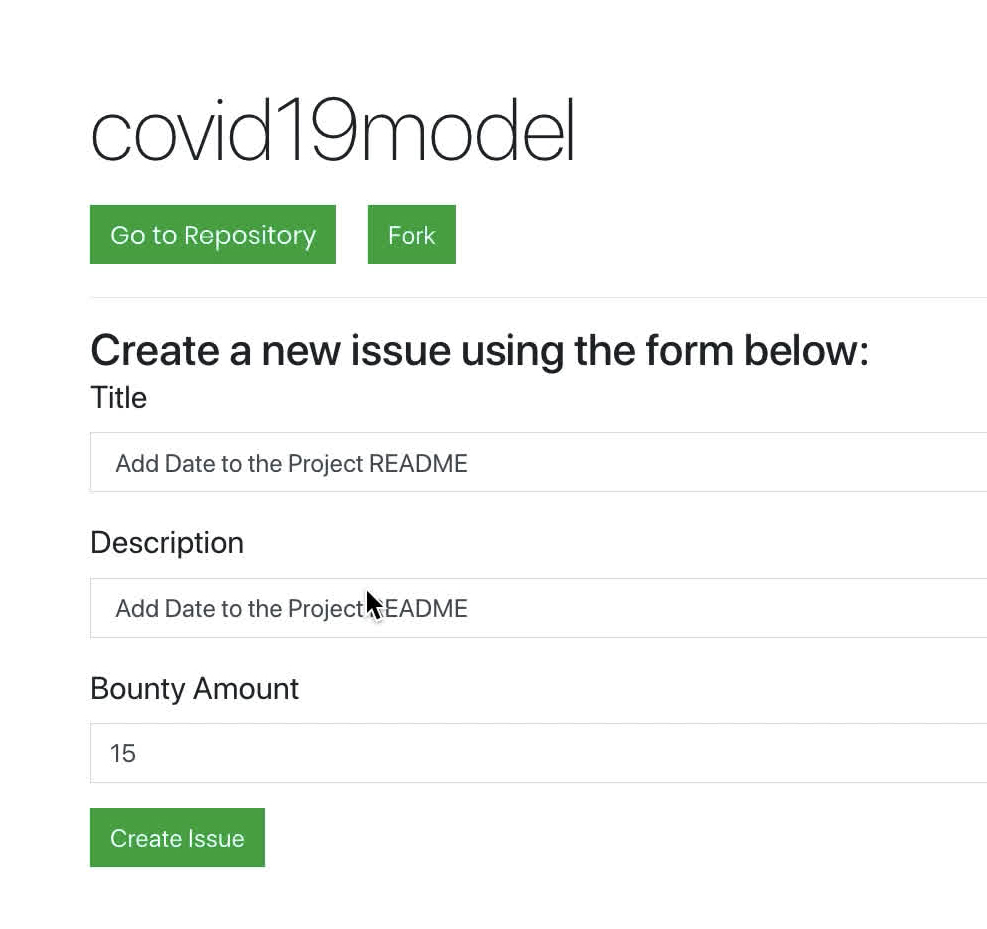
\includegraphics[height=7cm]{graphs/26. alice_create_issue1}

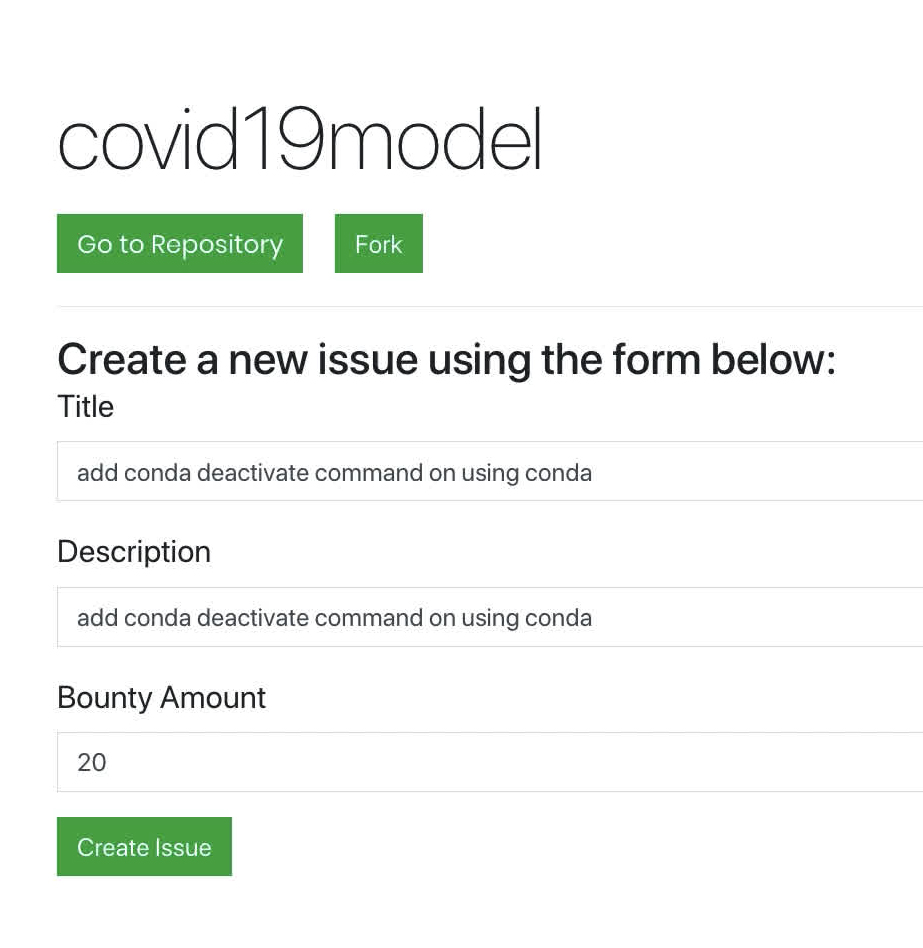
\includegraphics[height=7cm]{graphs/27. alice_create_issue2}

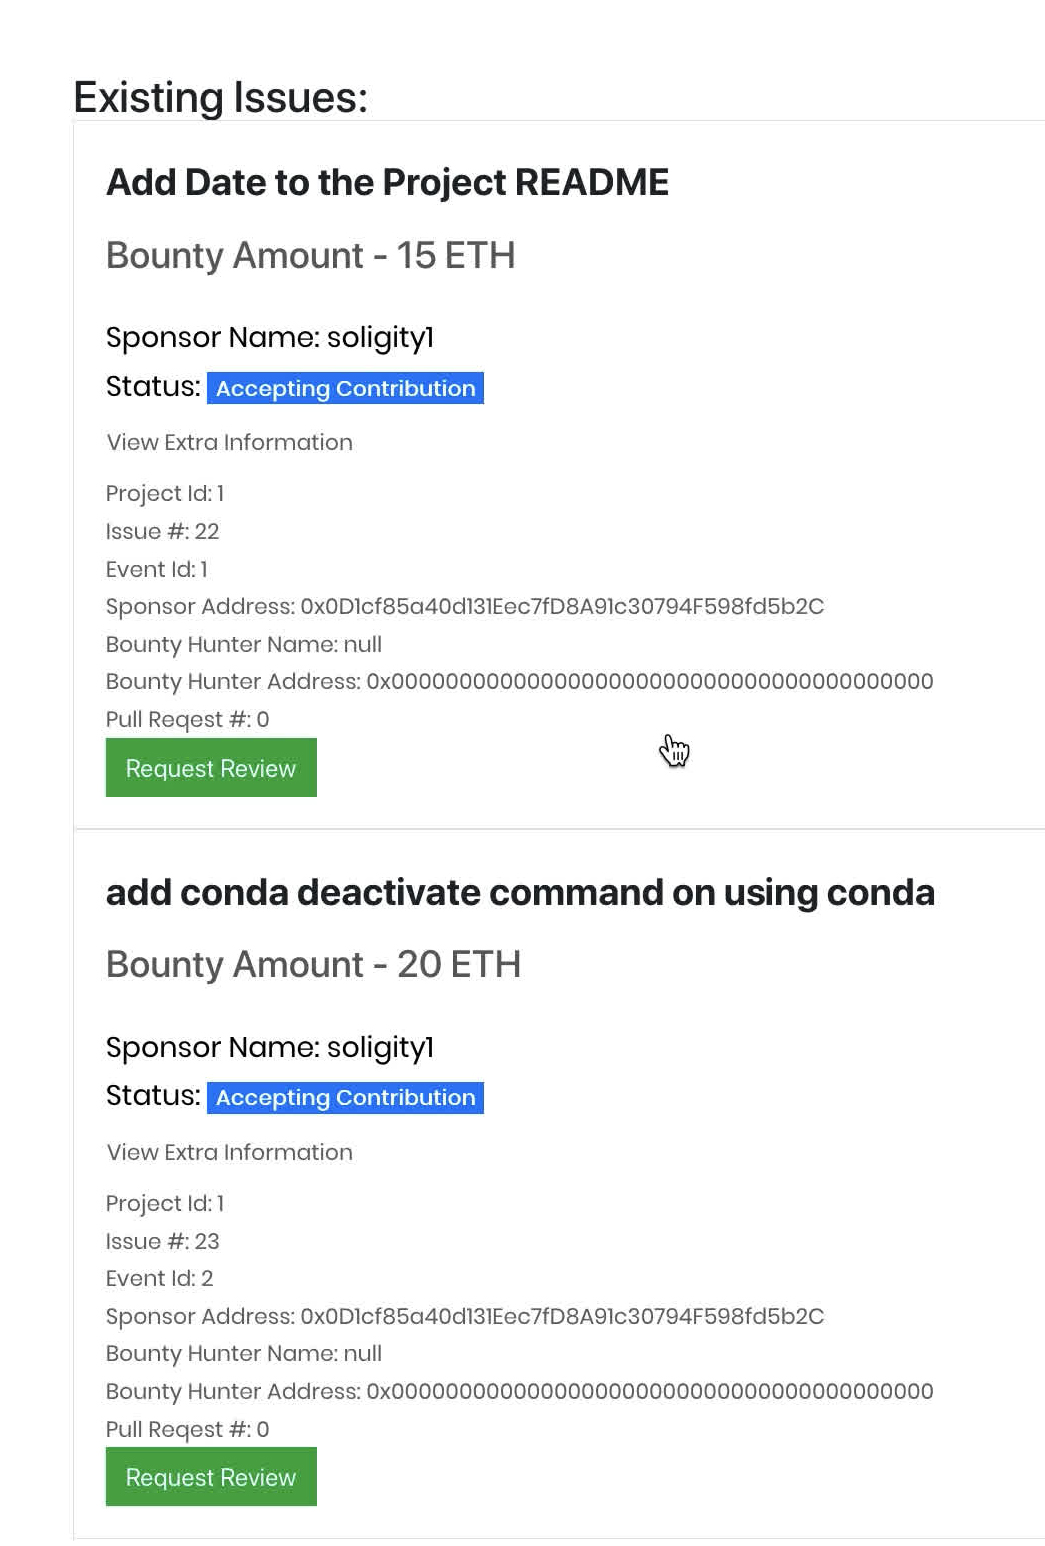
\includegraphics[height=7cm]{graphs/28. soligity_issues}

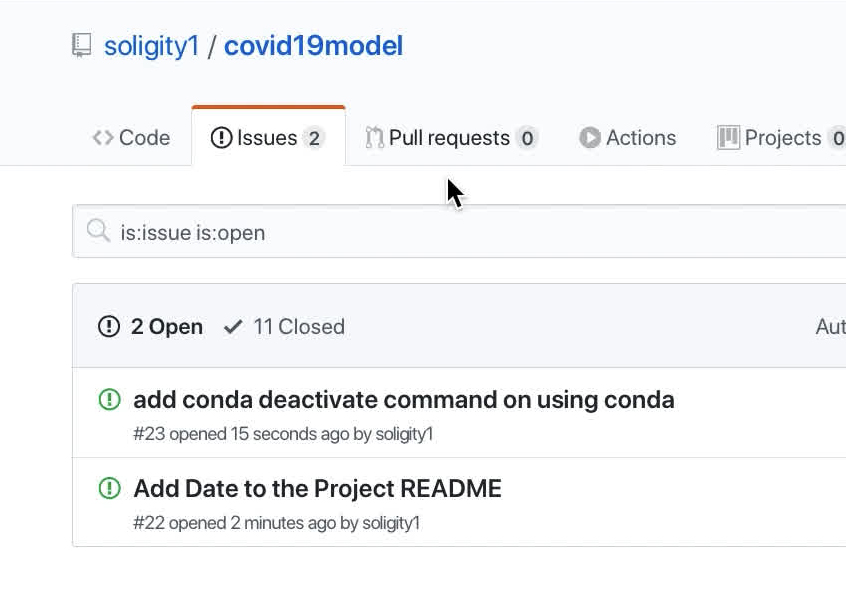
\includegraphics[height=7cm]{graphs/29. github_issues}

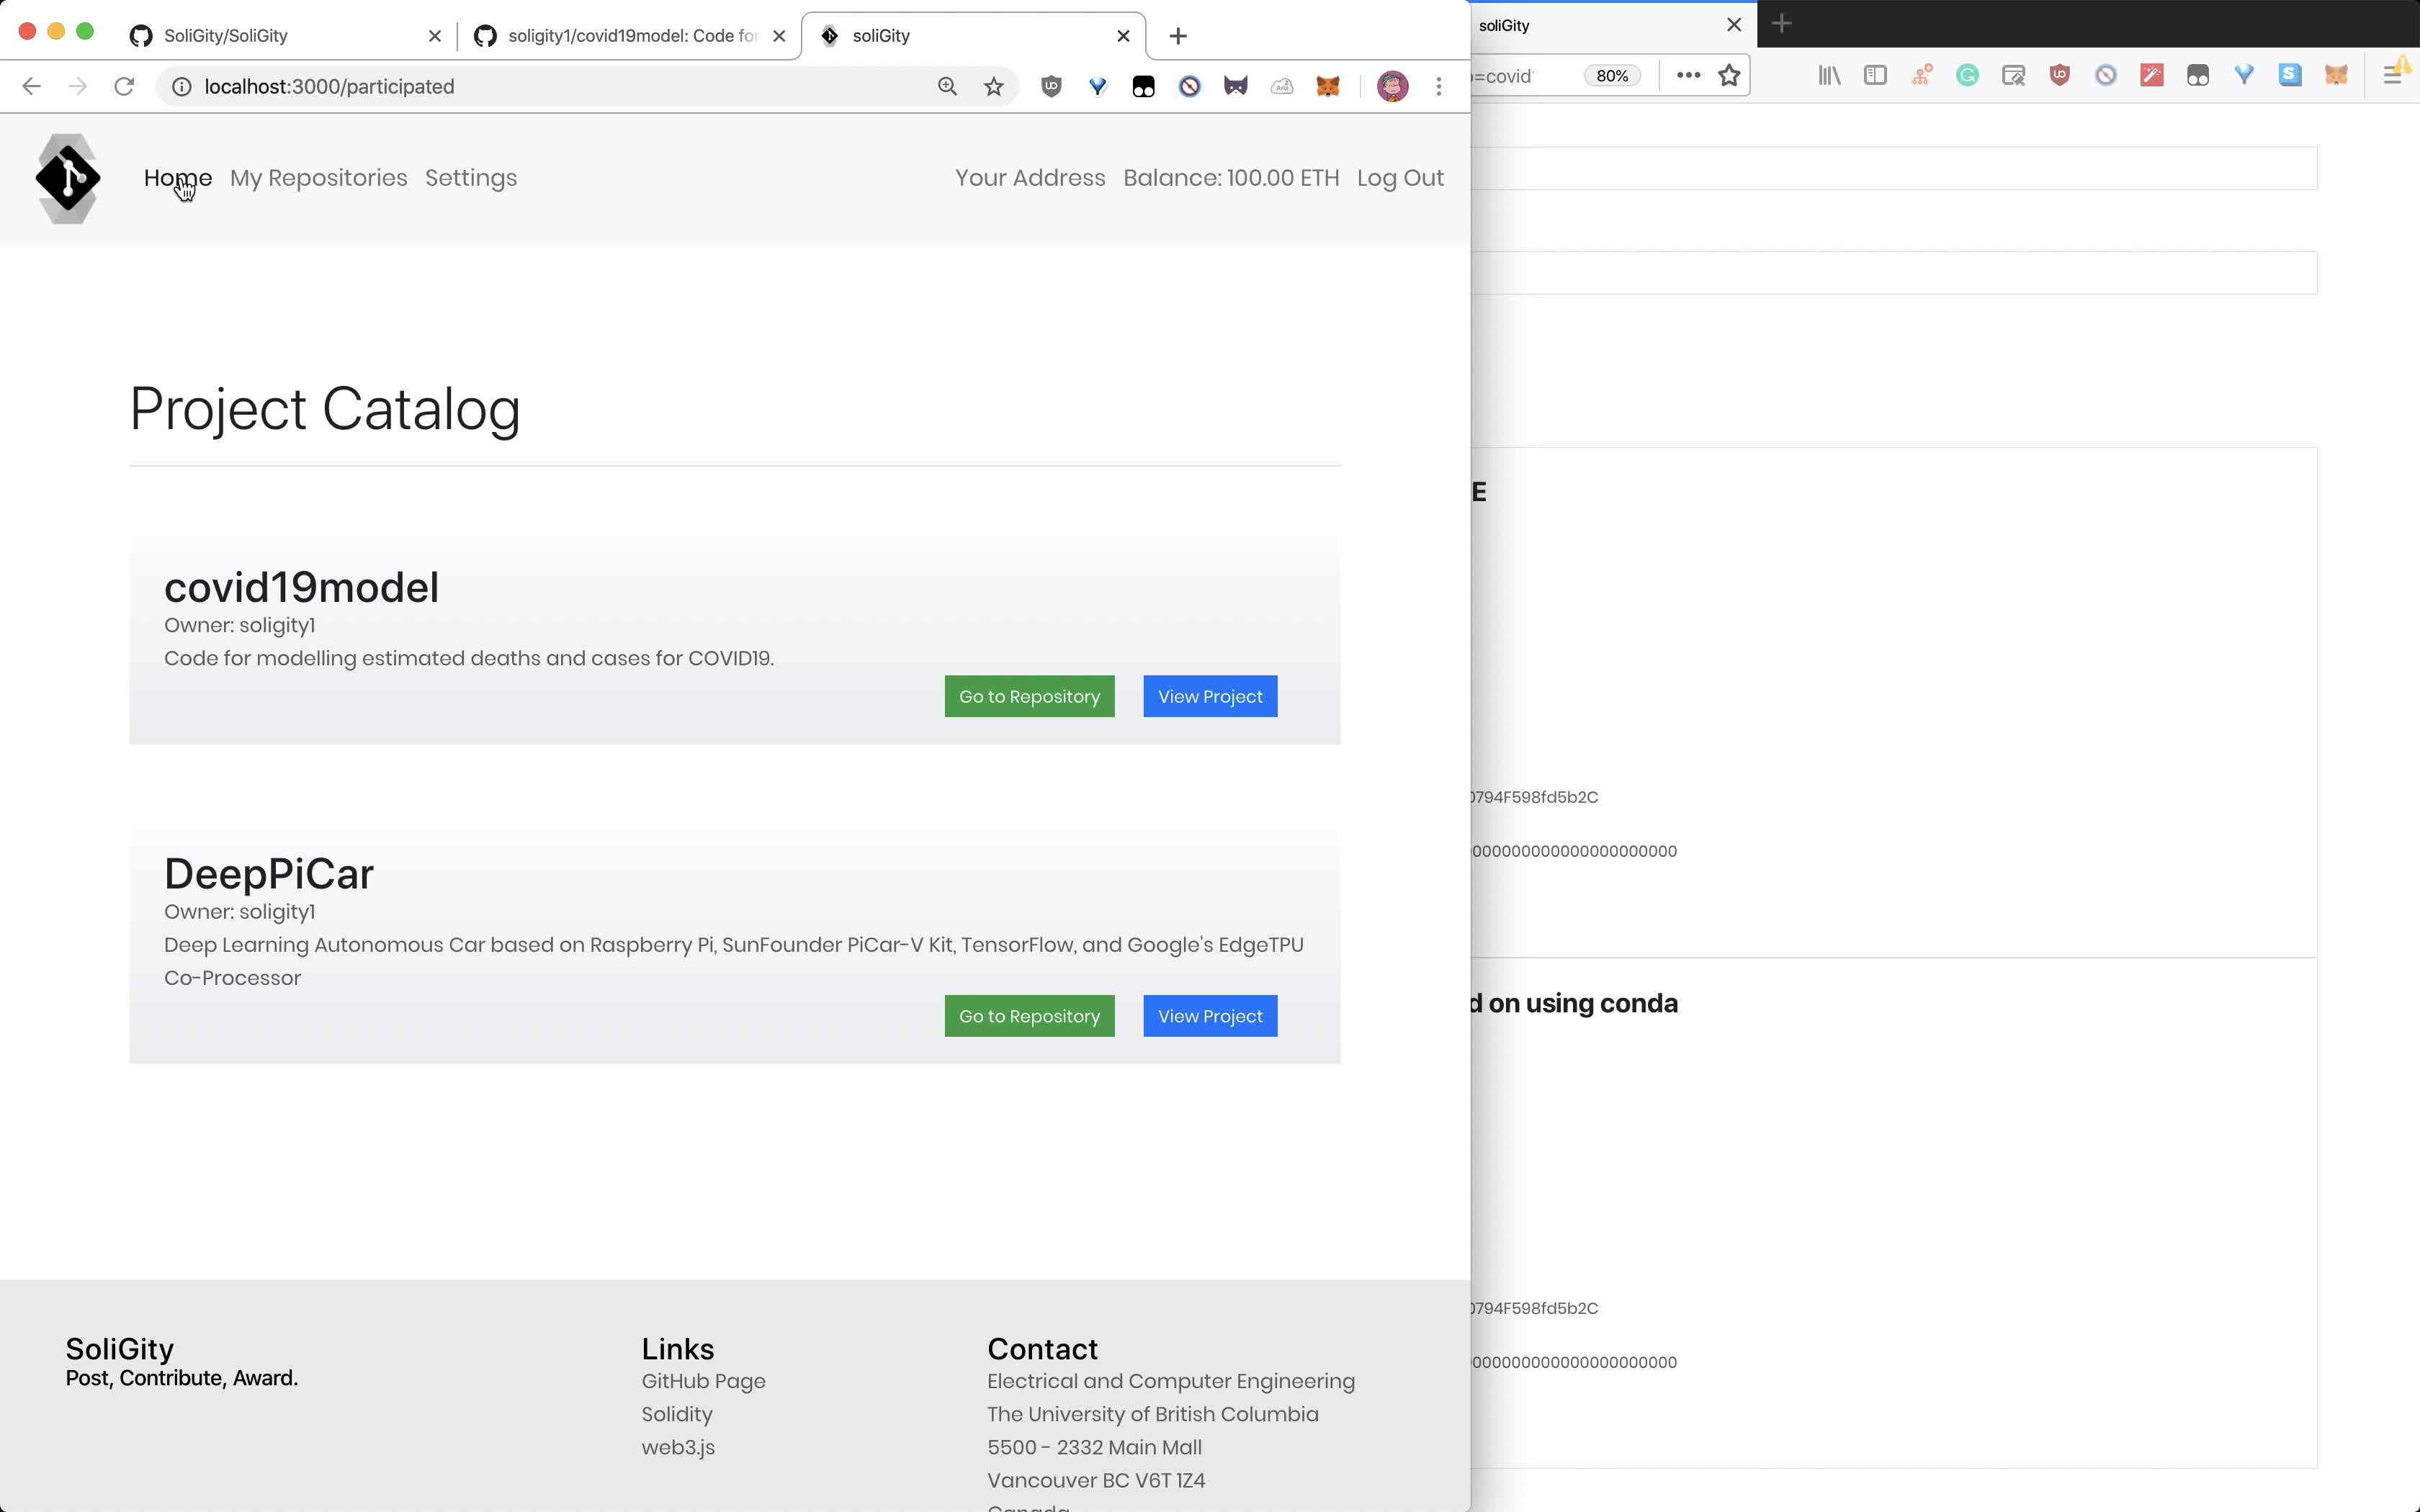
\includegraphics[height=7cm]{graphs/30. project_catalog_bob_view}


\includegraphics[height=7cm]{graphs/31. bob_fork_project}

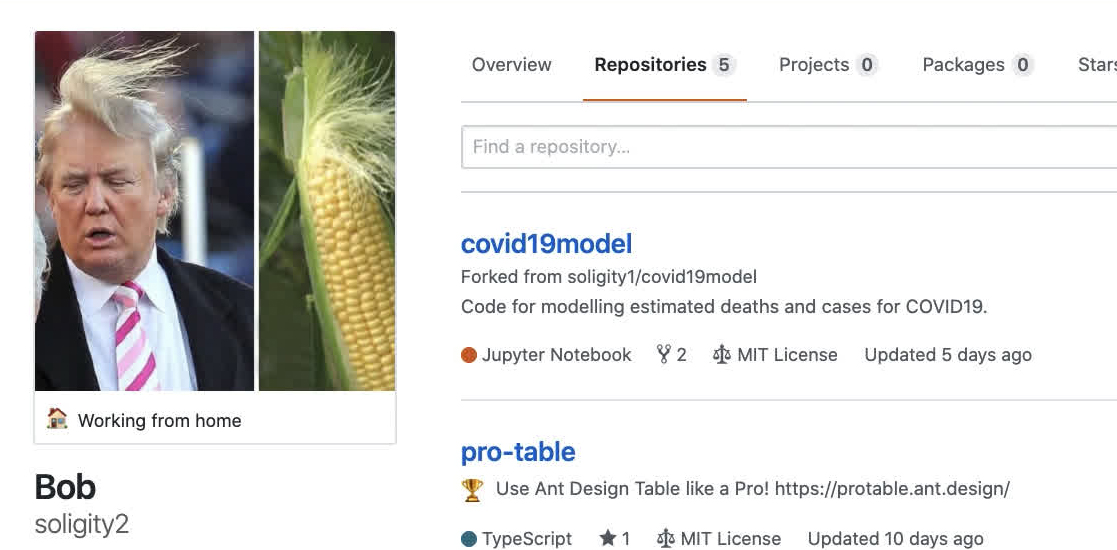
\includegraphics[height=7cm]{graphs/32. bob_forked_github}

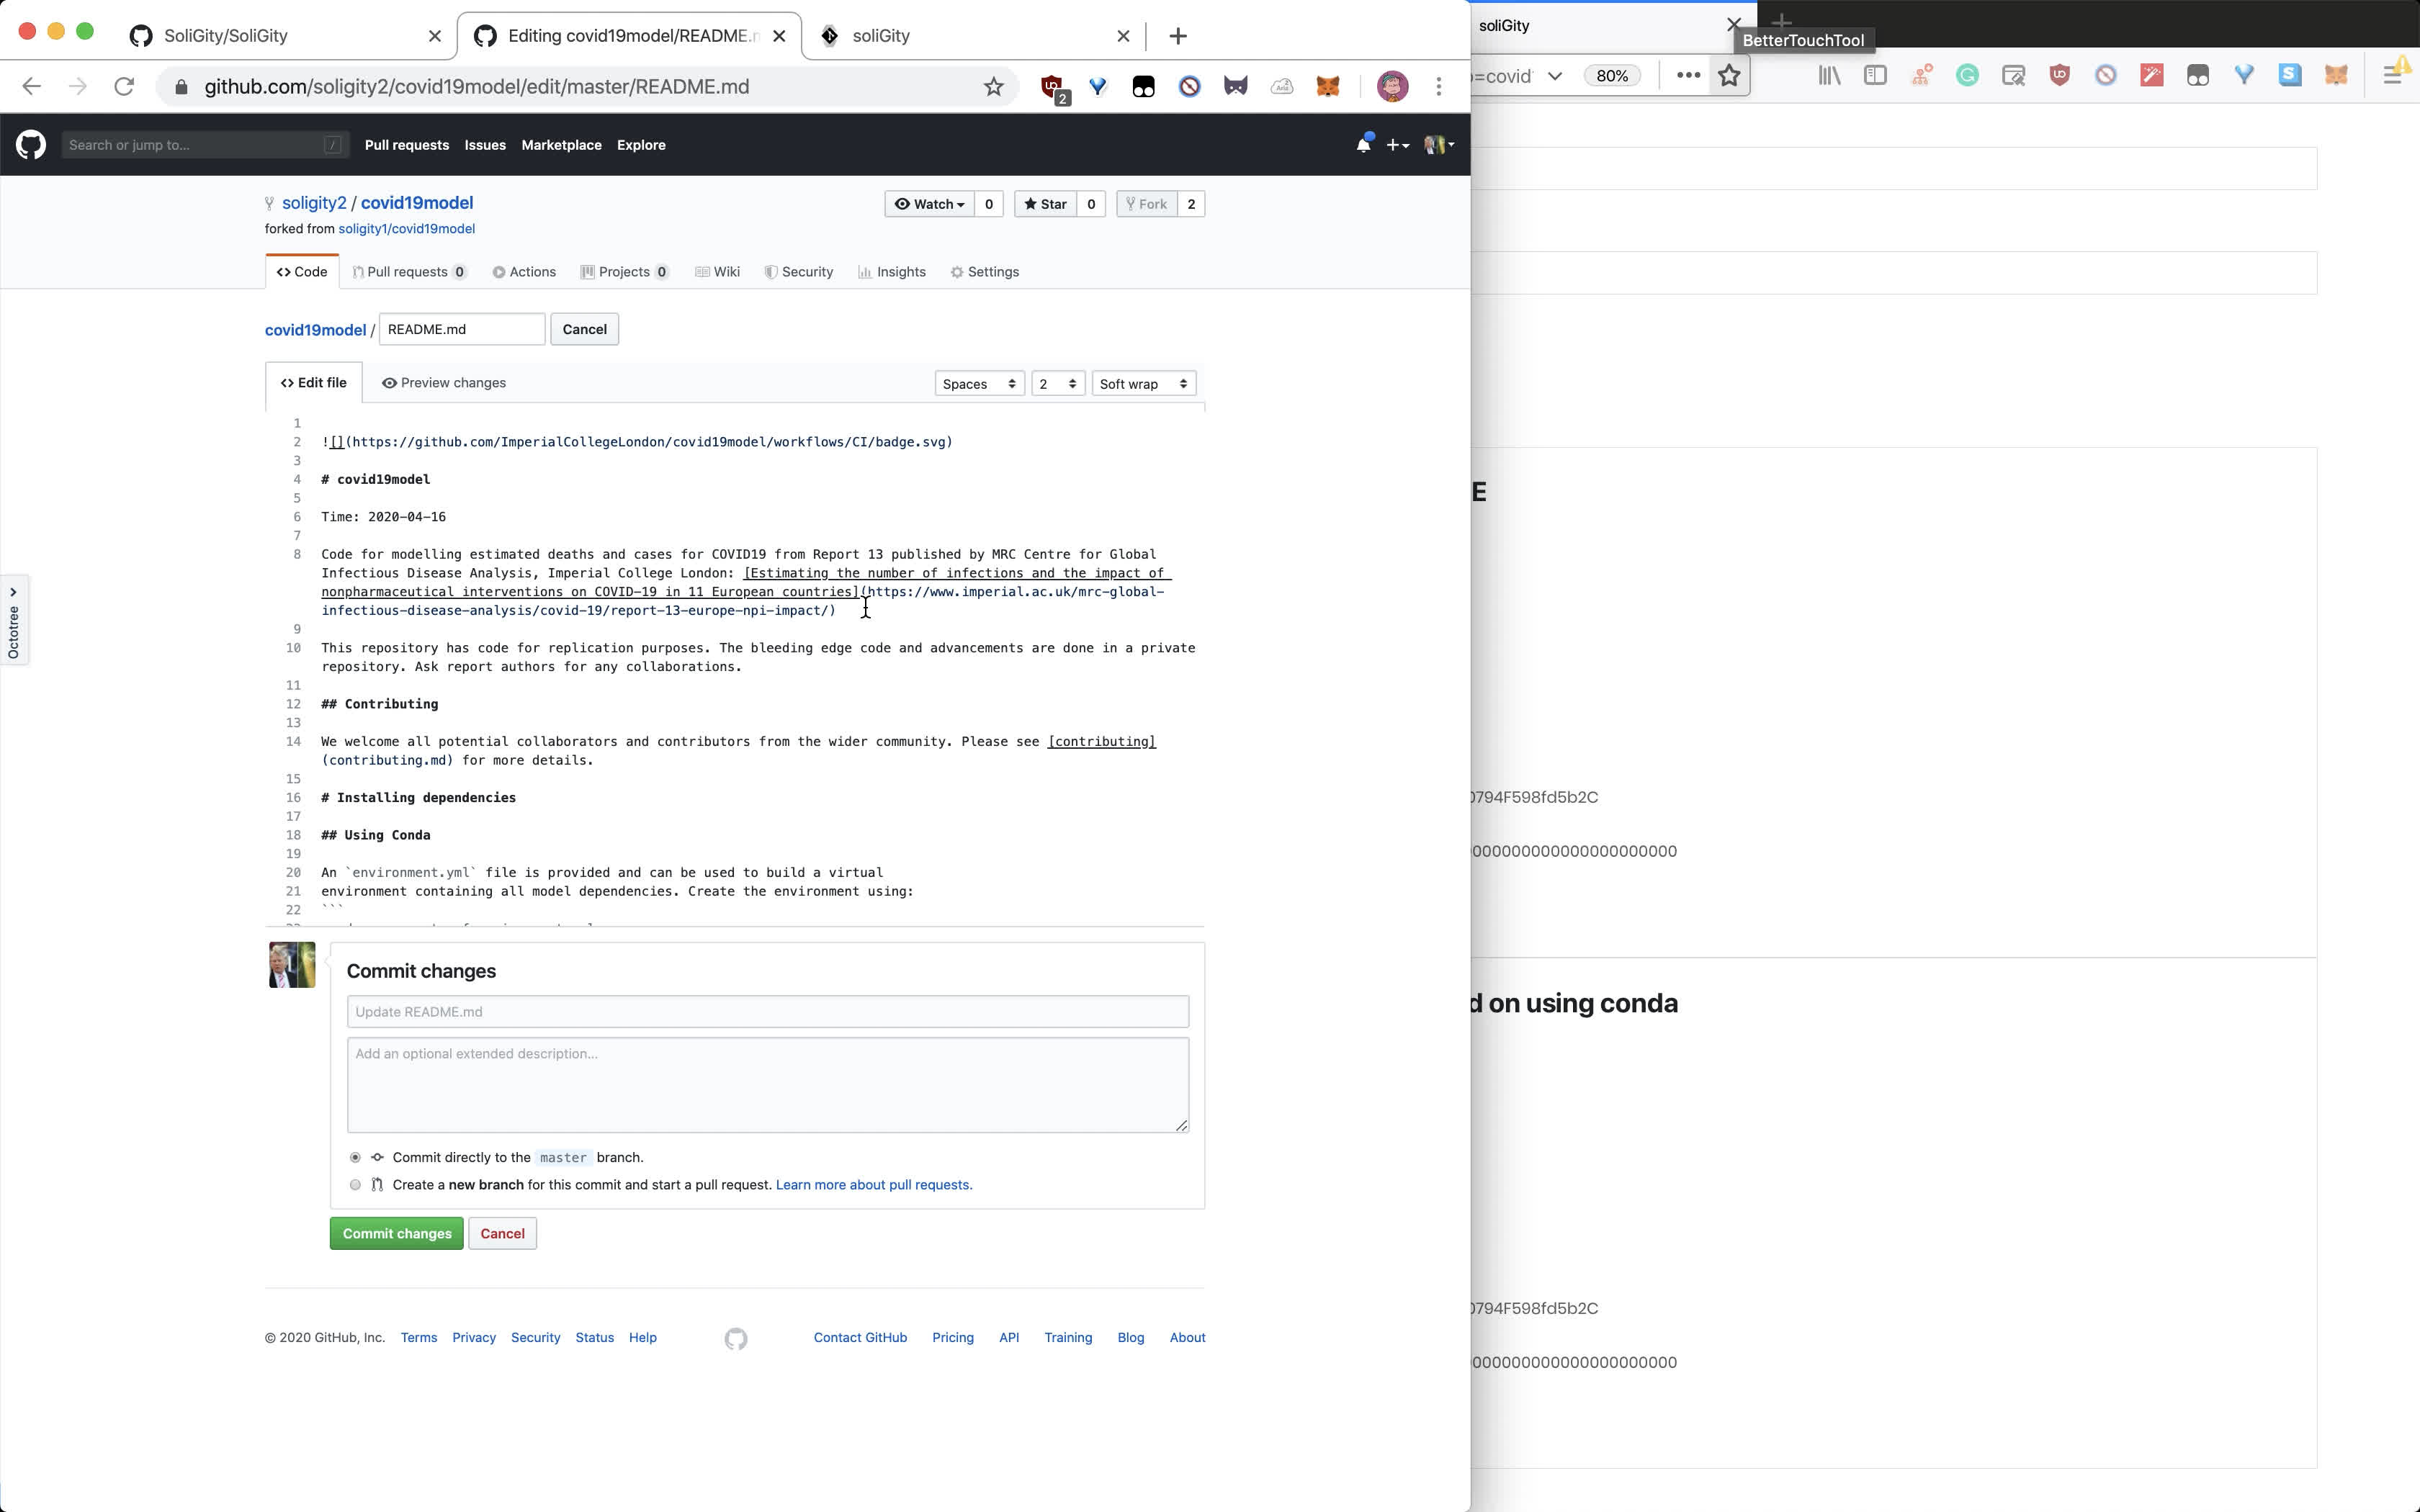
\includegraphics[height=7cm]{graphs/33. bob_make_changes}

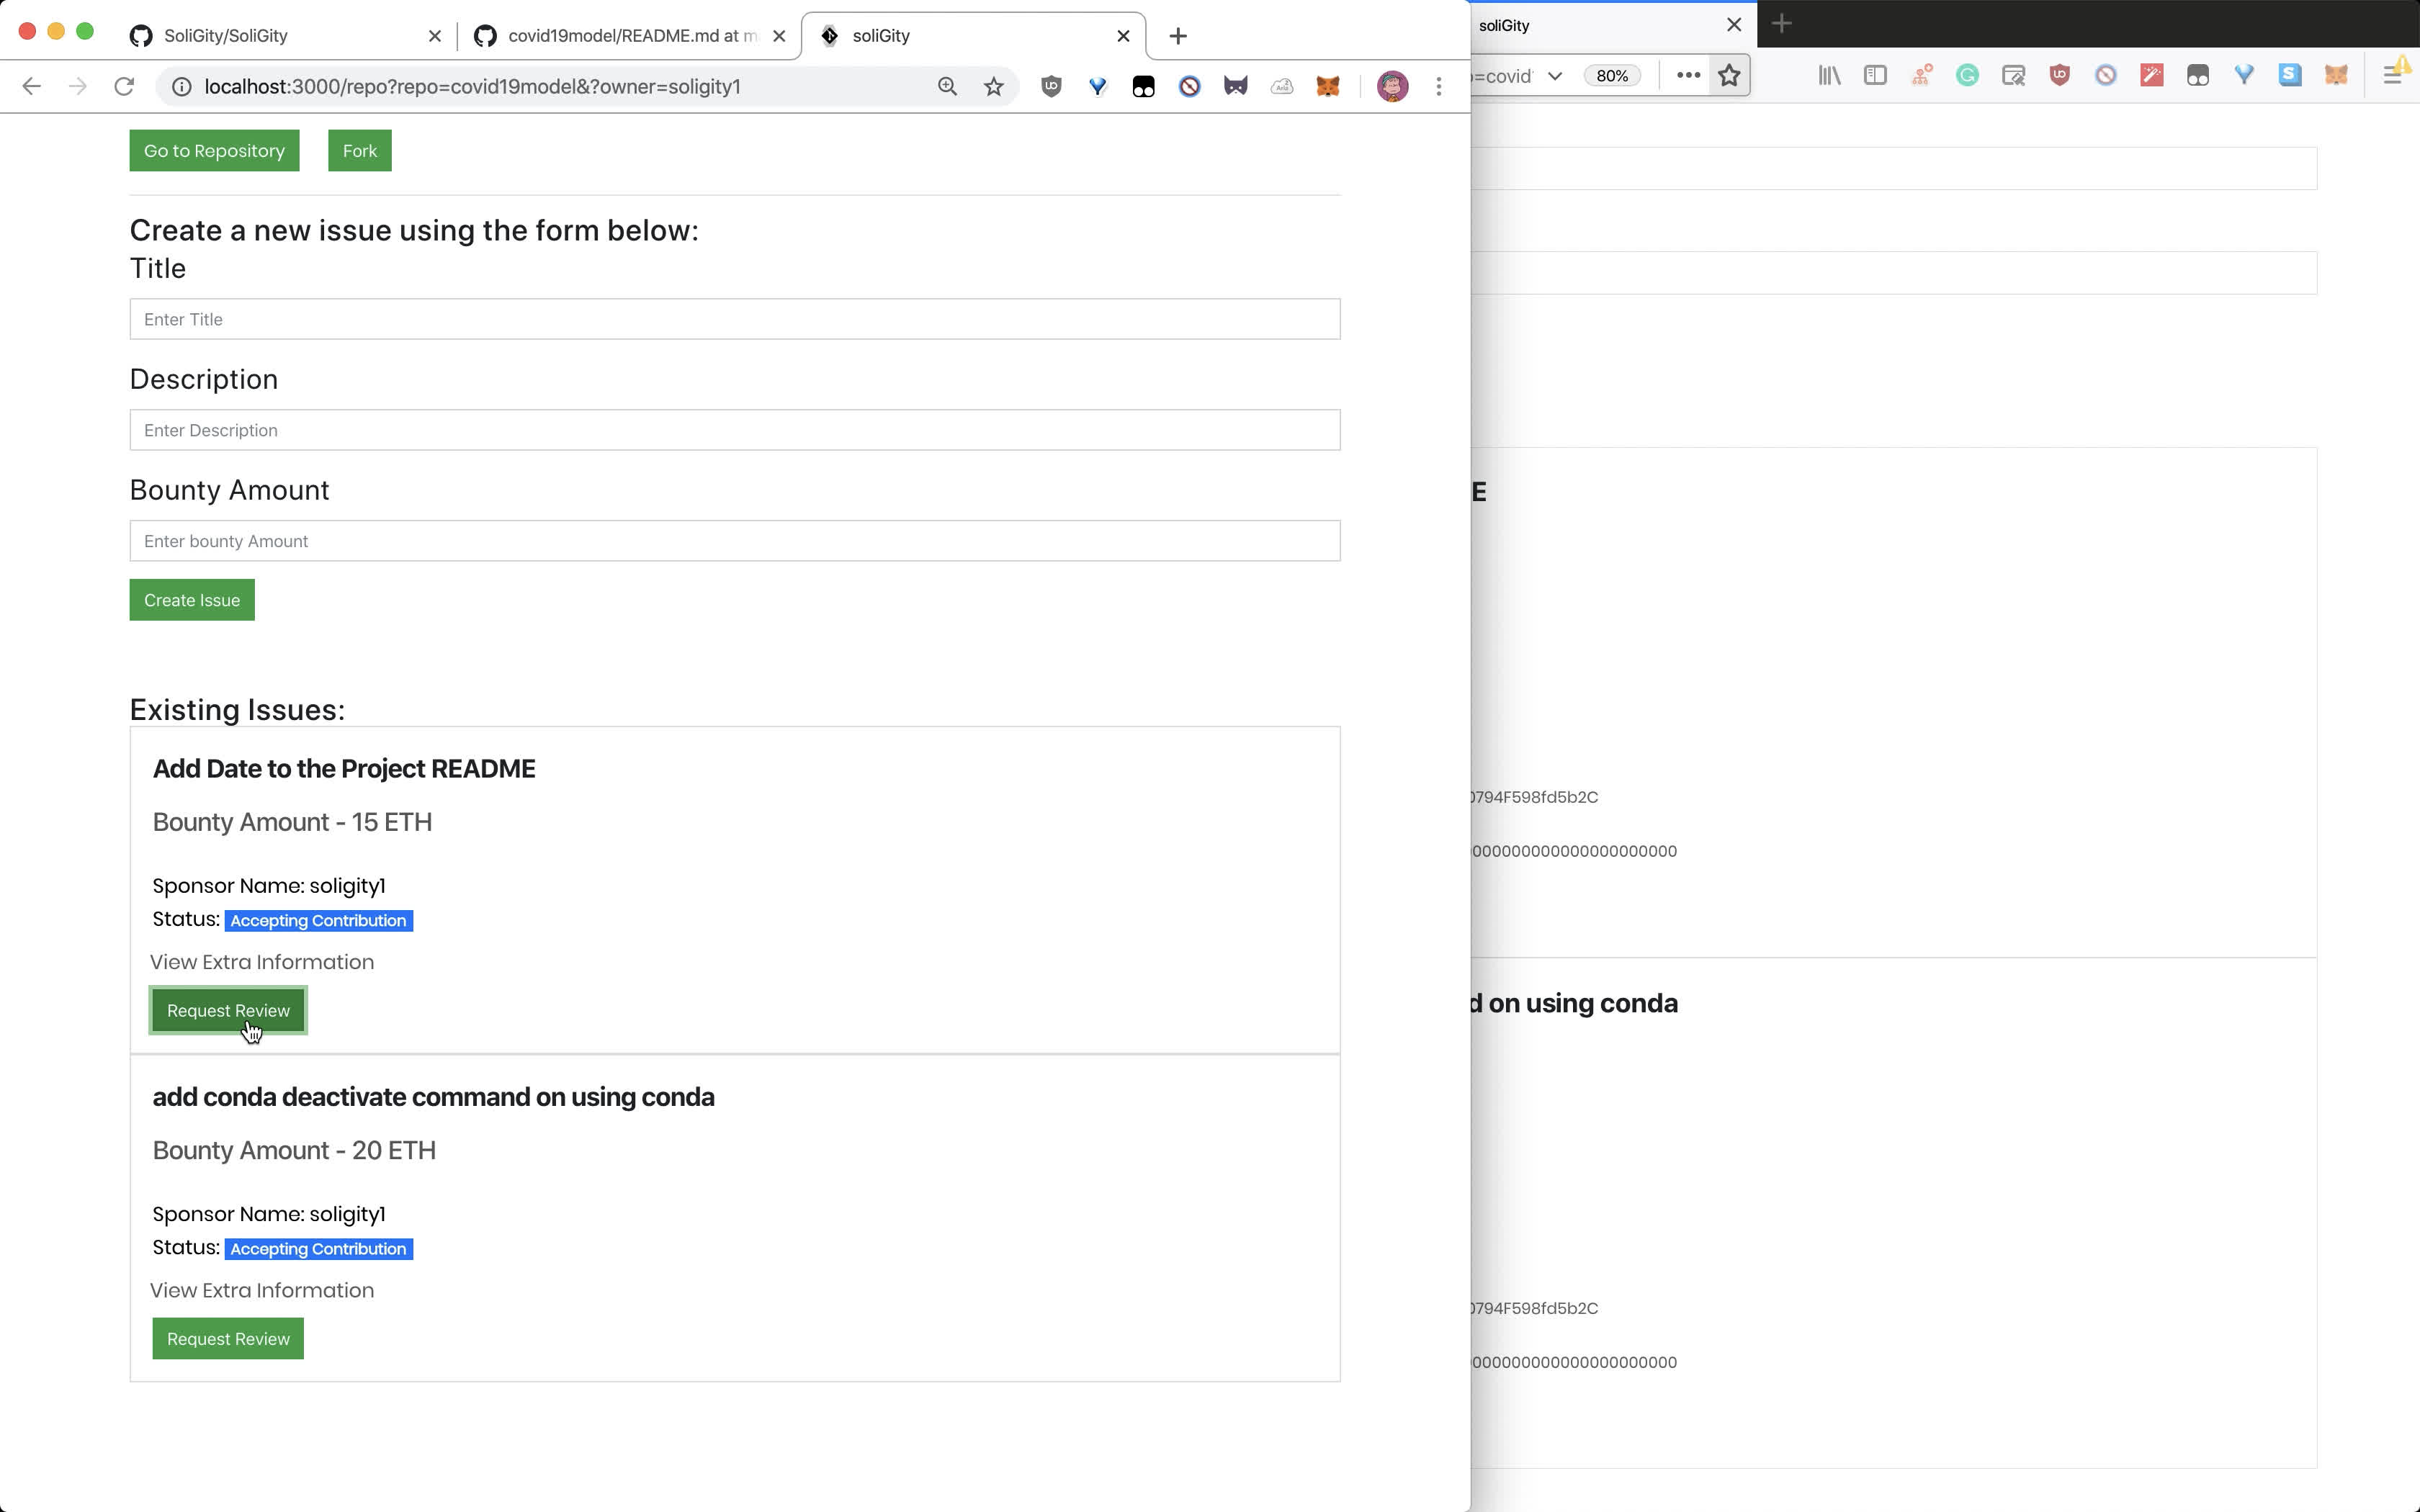
\includegraphics[height=7cm]{graphs/34. bob_review_request}

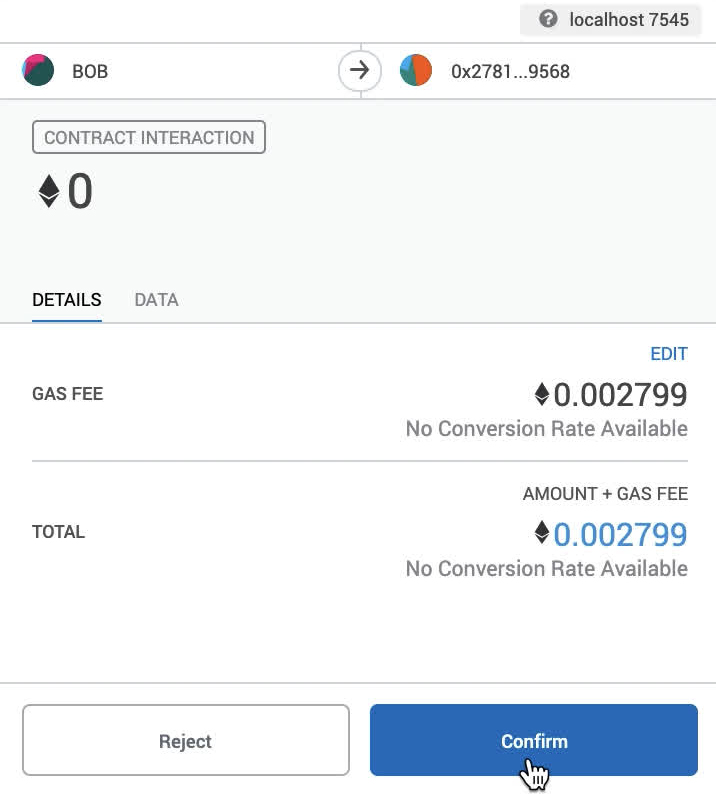
\includegraphics[height=7cm]{graphs/35. bob_review_request_metamask}

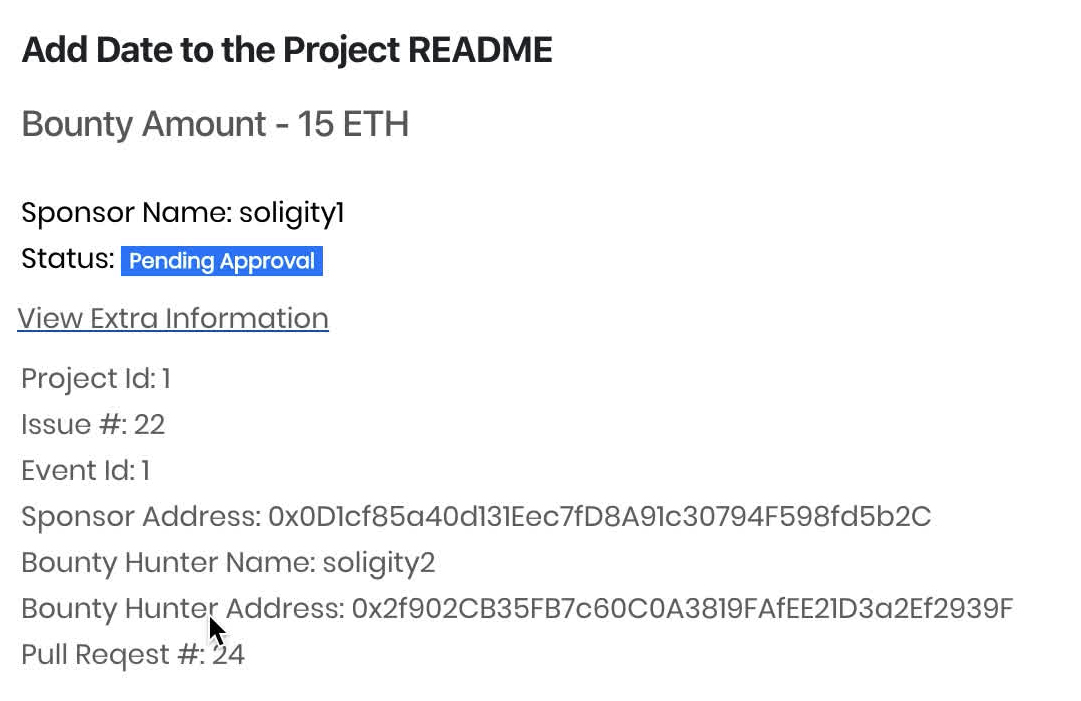
\includegraphics[height=7cm]{graphs/36. issue_info_updated}

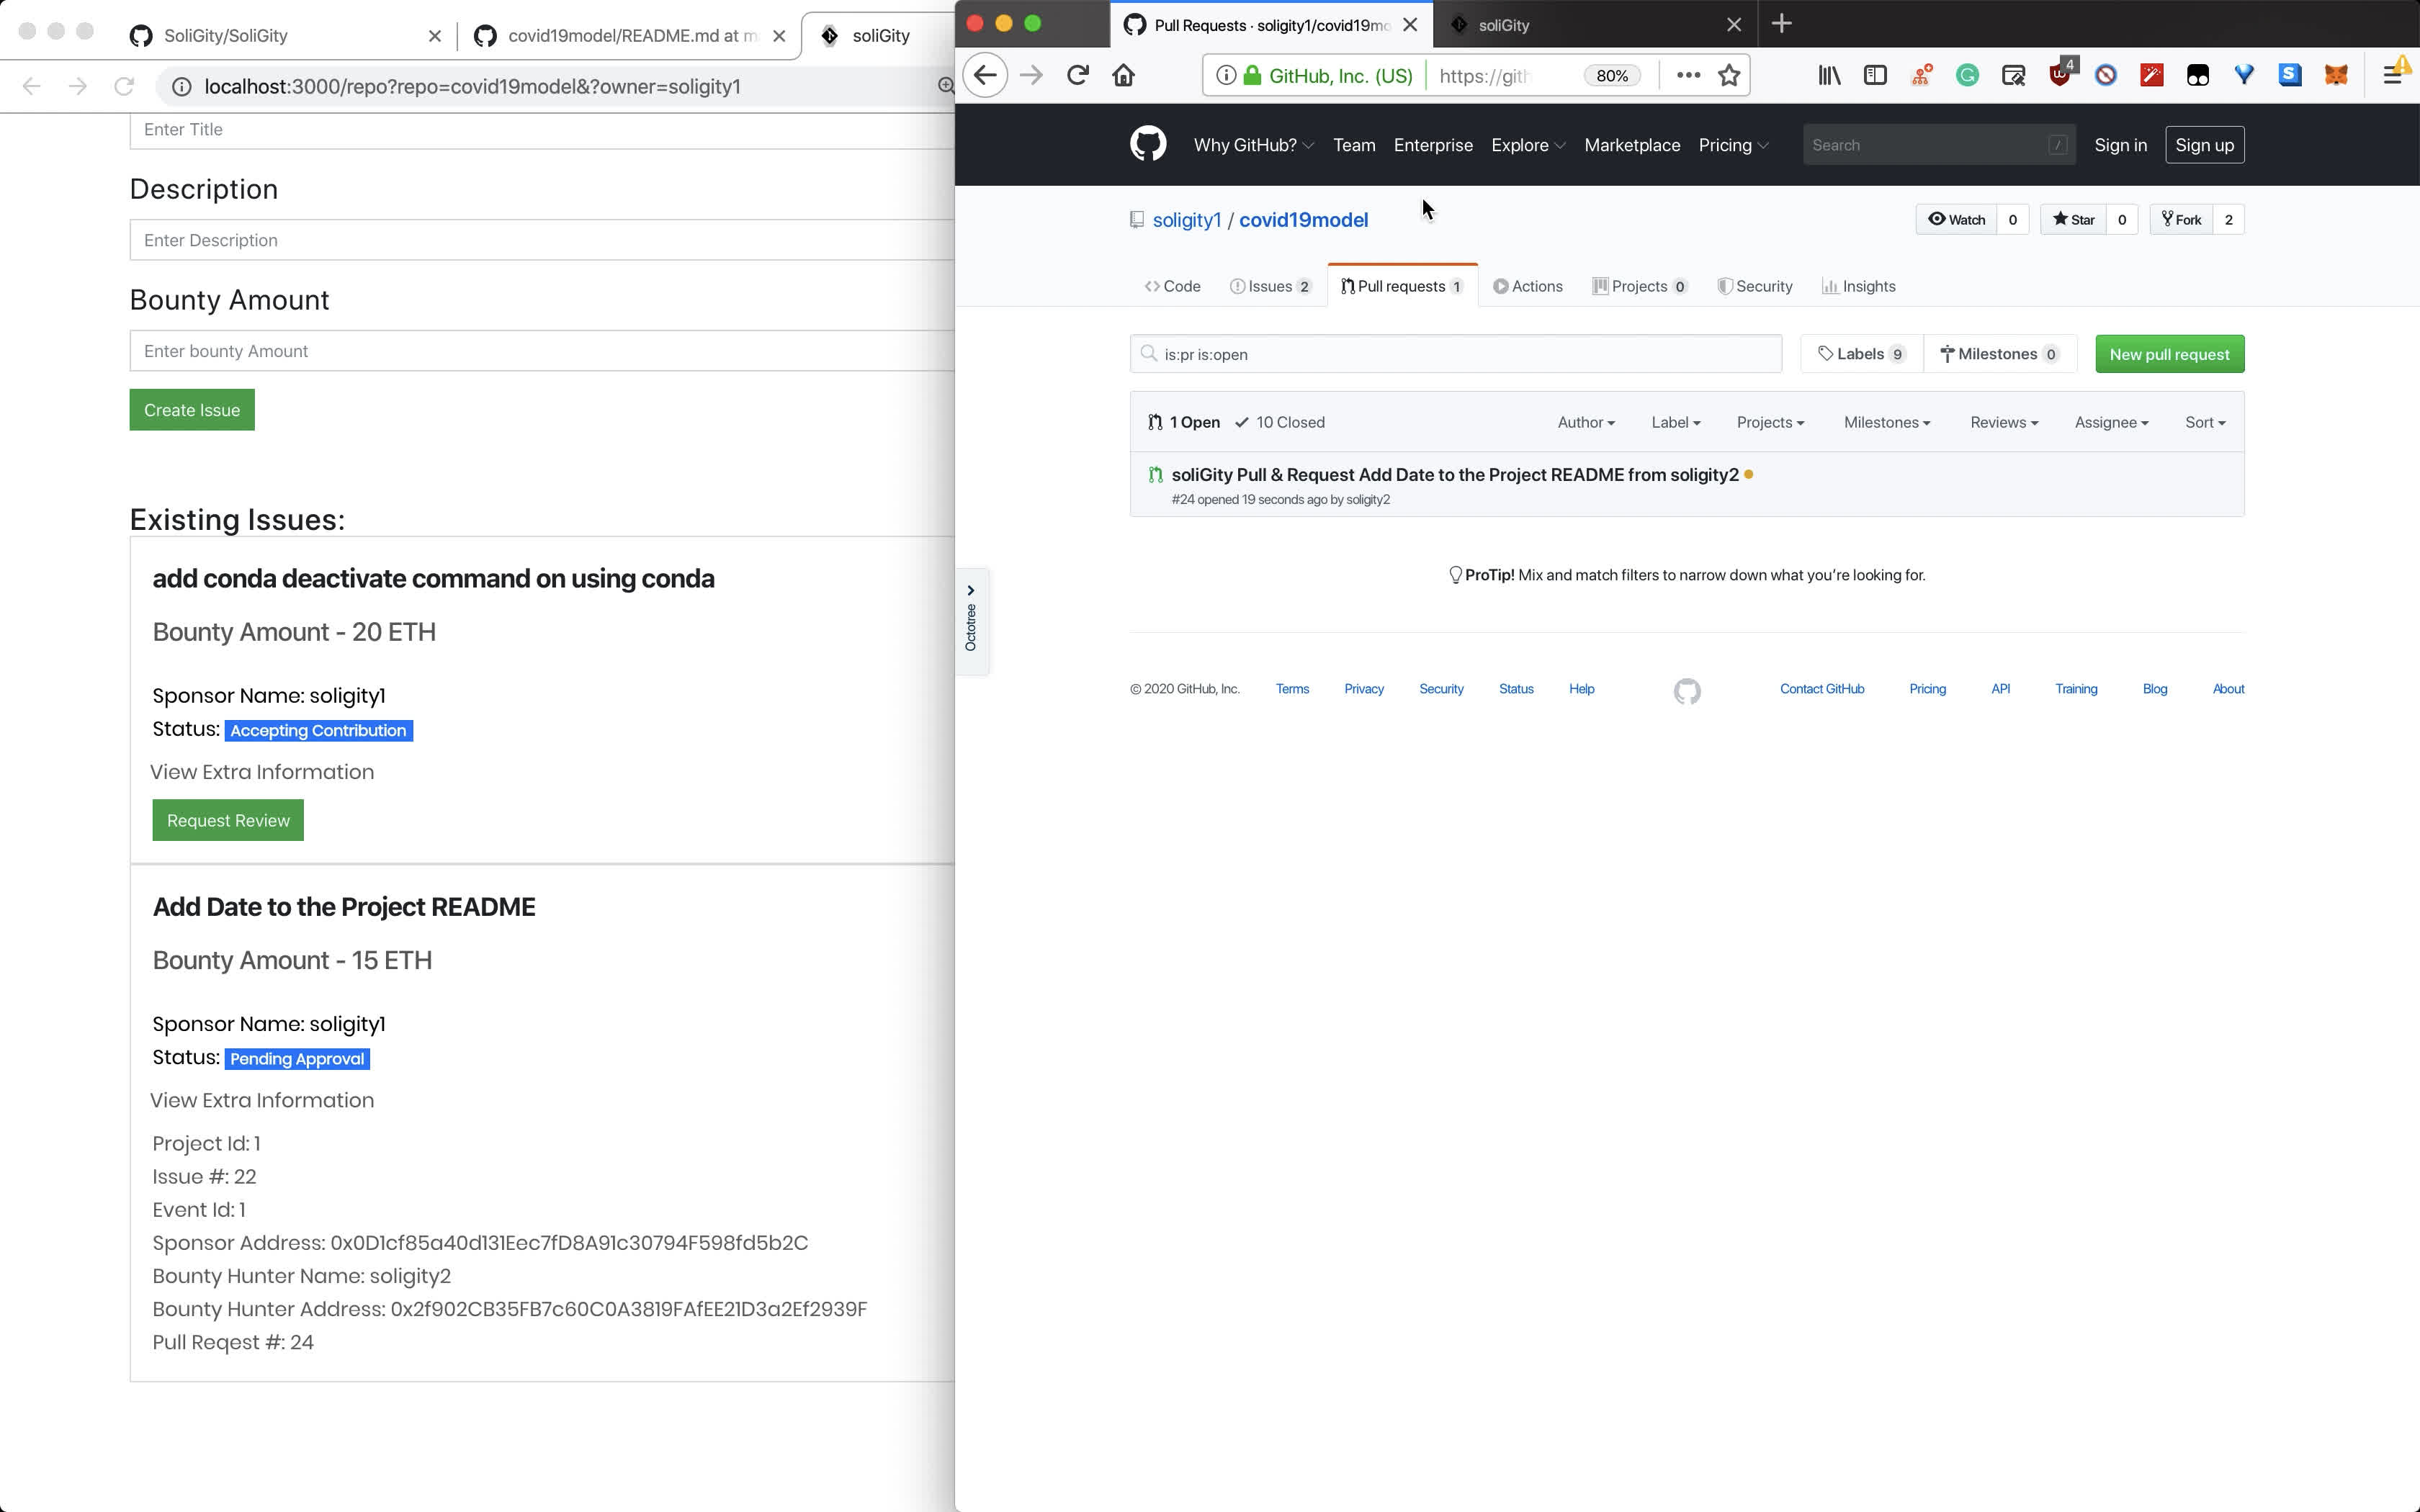
\includegraphics[height=7cm]{graphs/37. bob_pull_request_github}

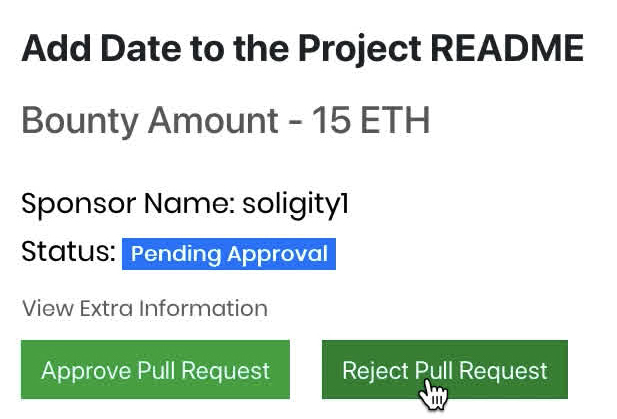
\includegraphics[height=7cm]{graphs/38. alice_reject_pull_request}

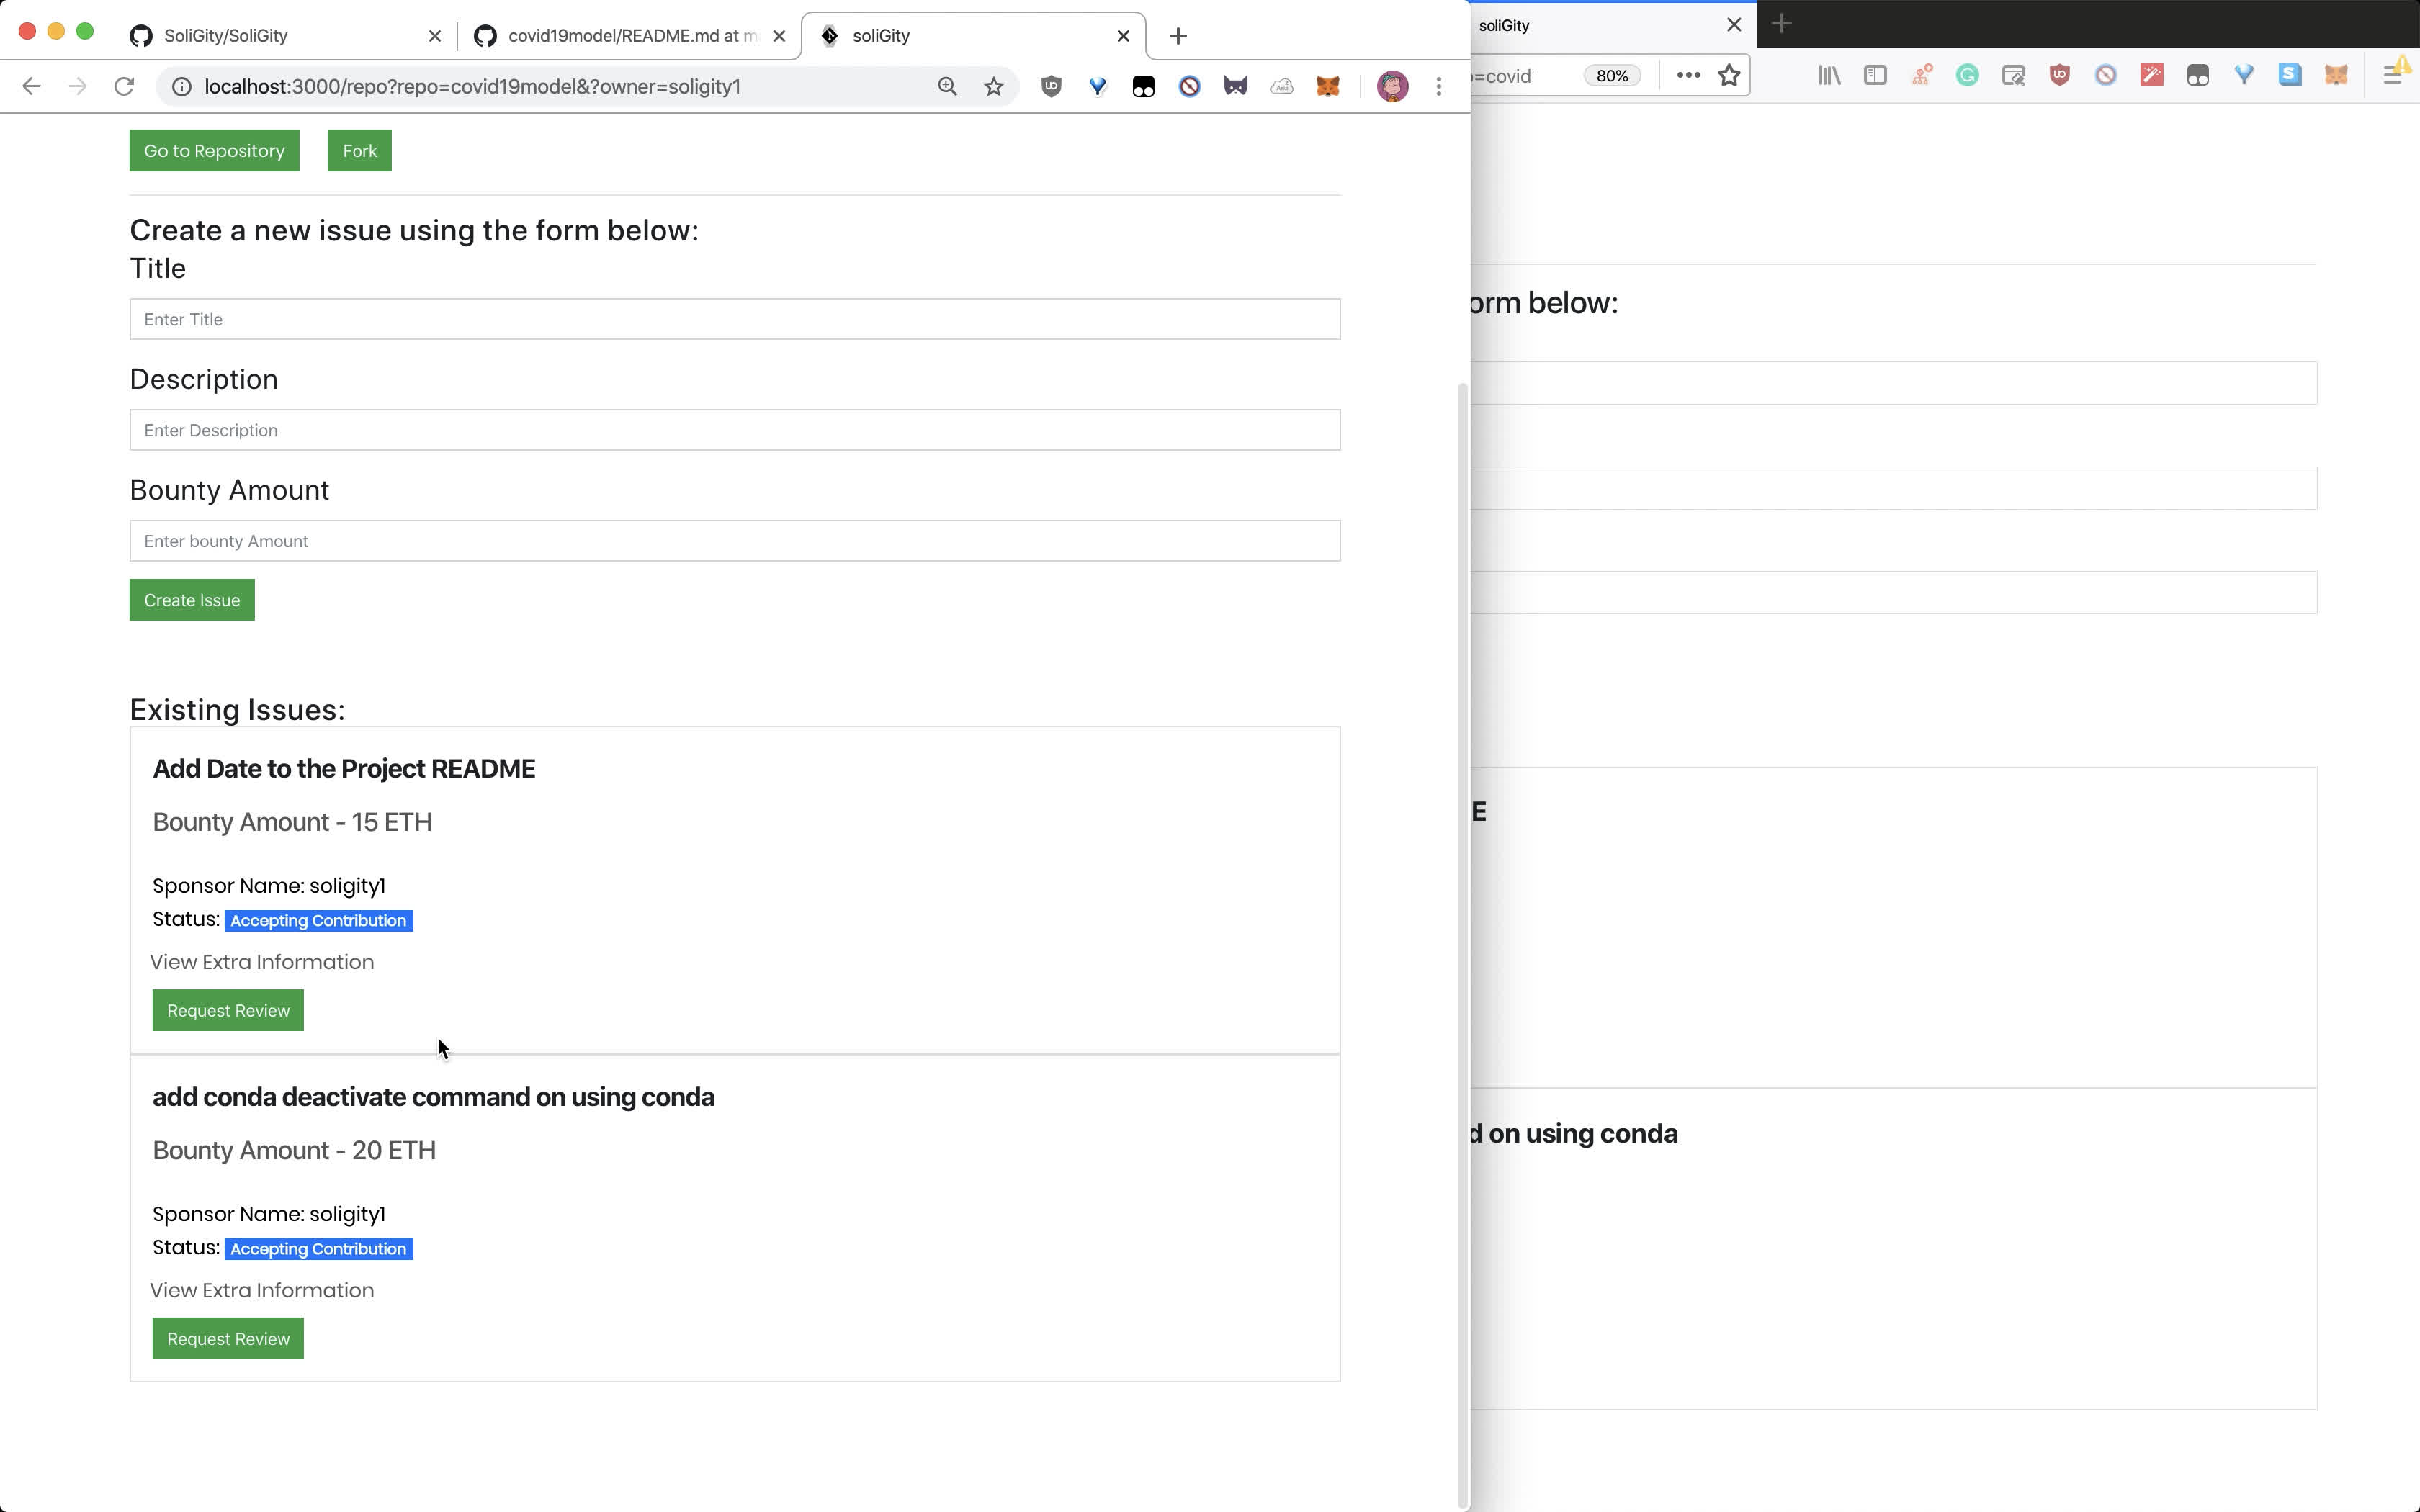
\includegraphics[height=7cm]{graphs/39. issue_info_updated}

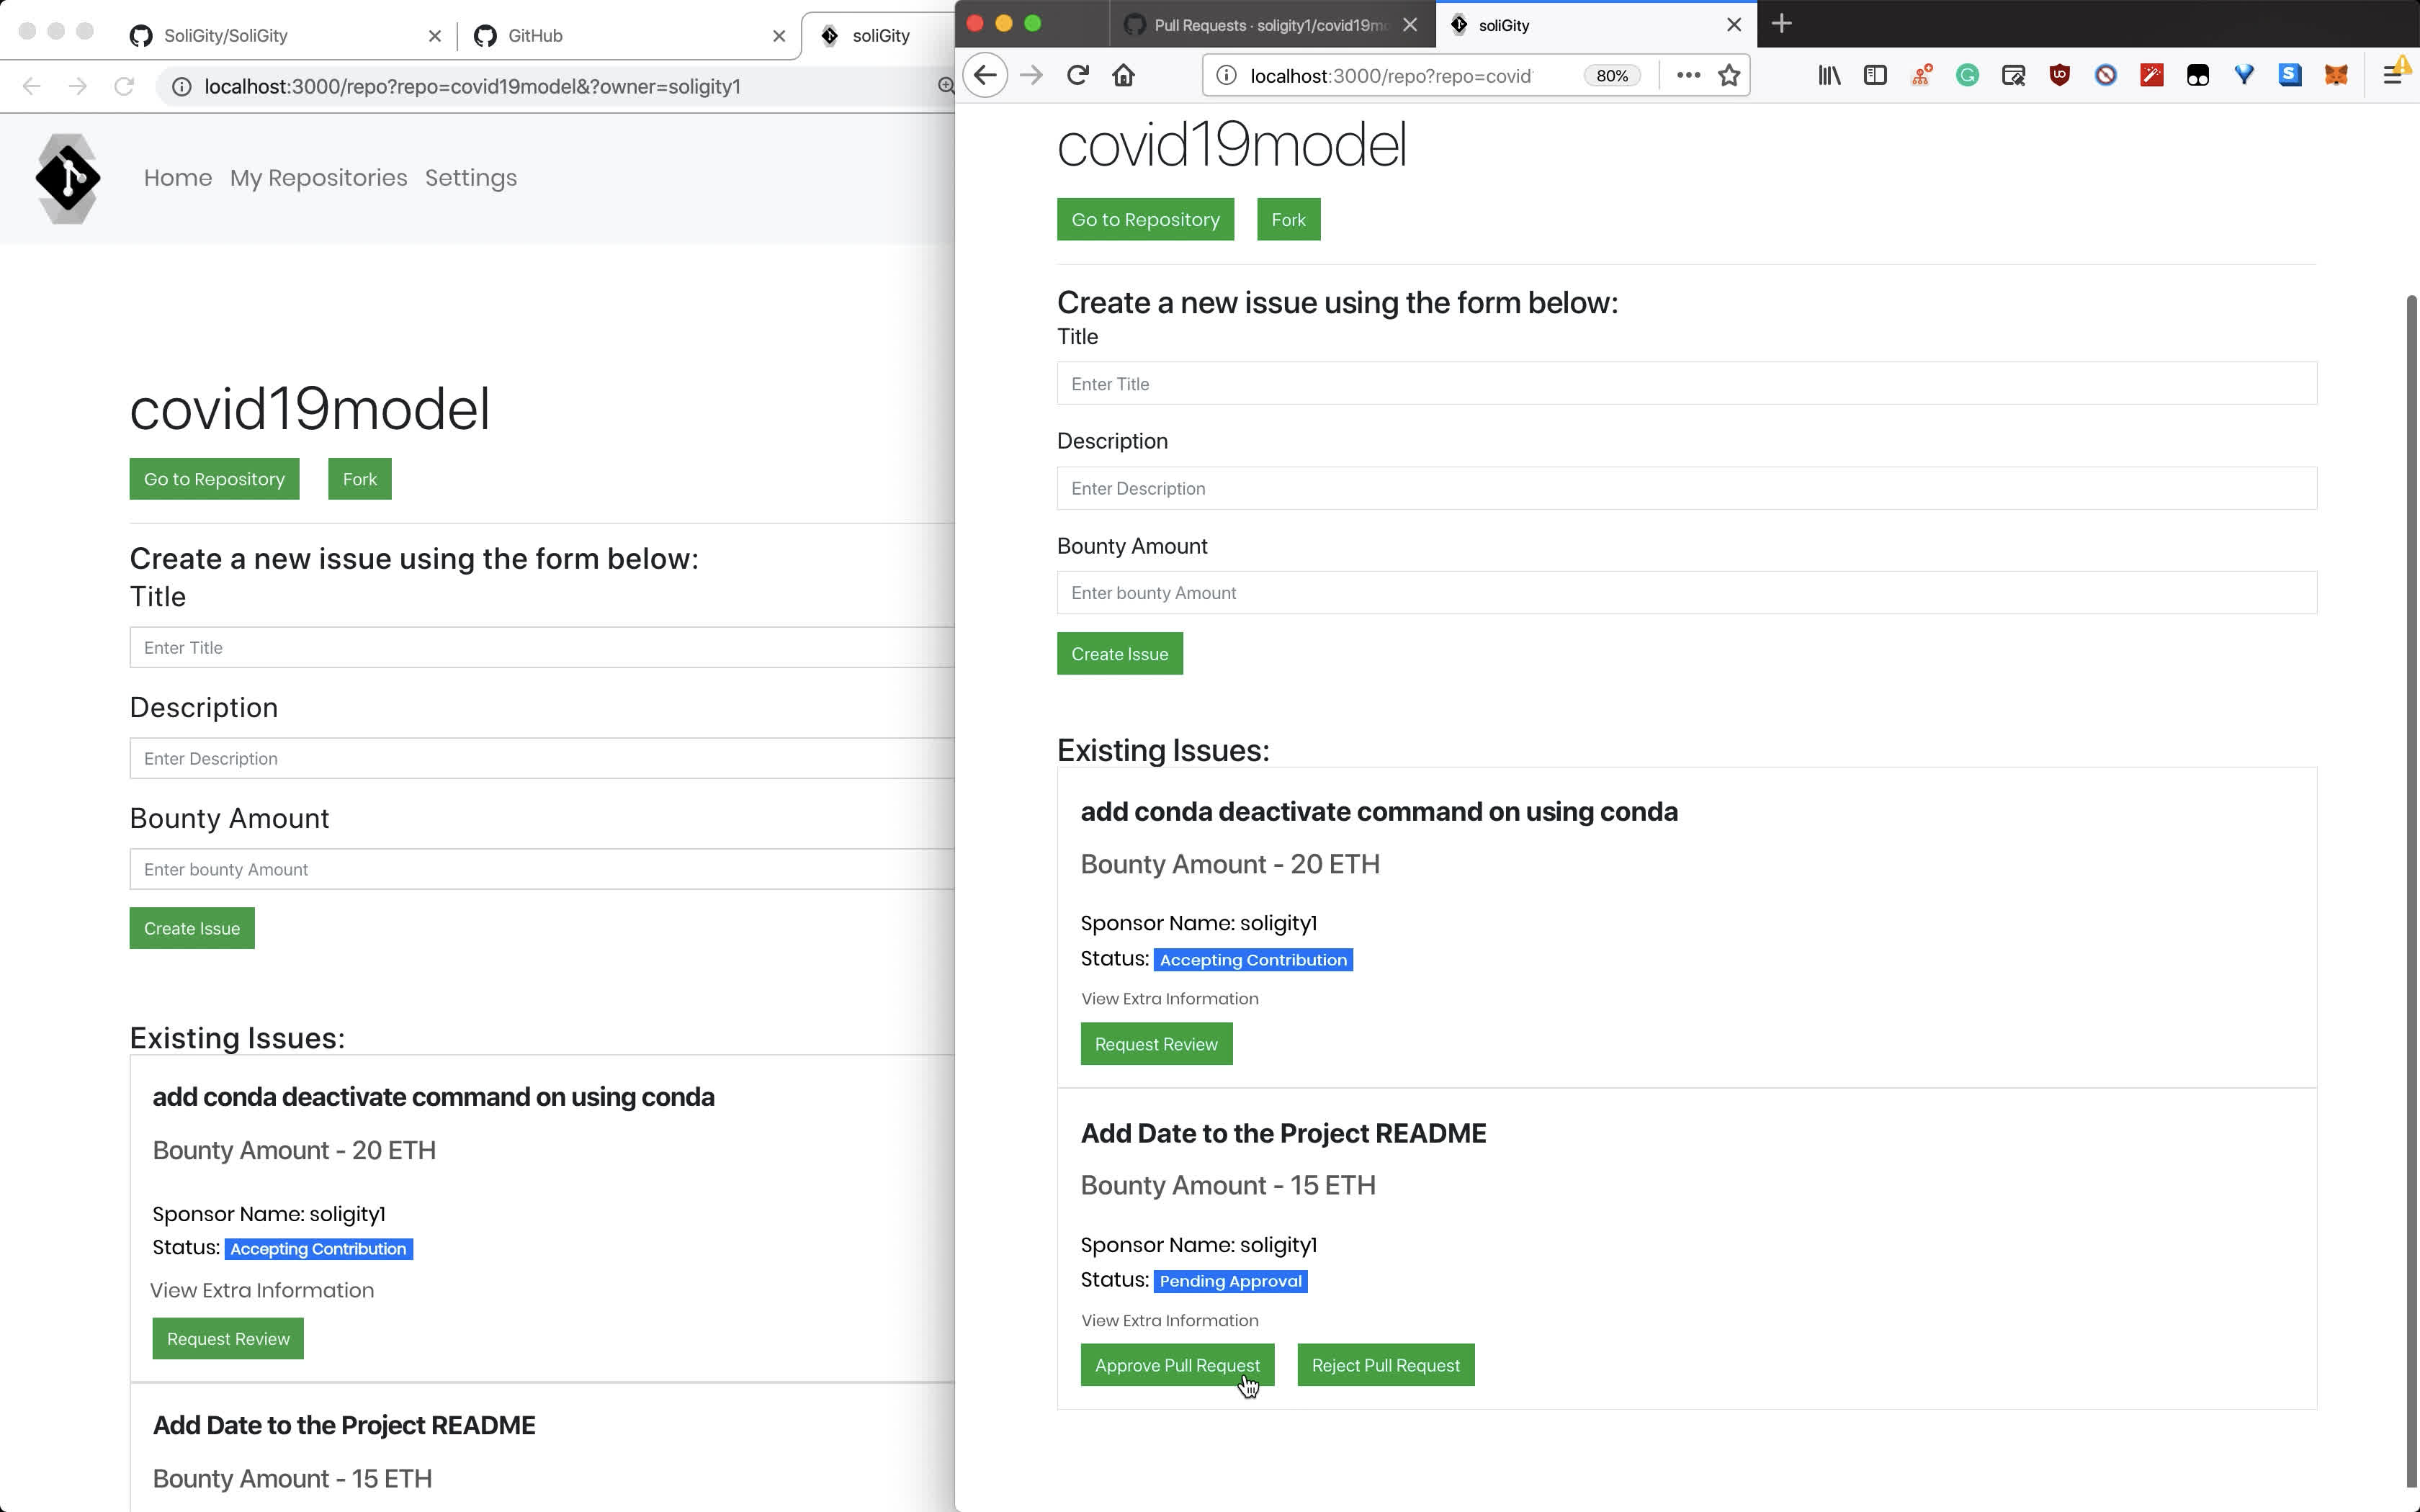
\includegraphics[height=7cm]{graphs/40. alice_approve_pull_request}

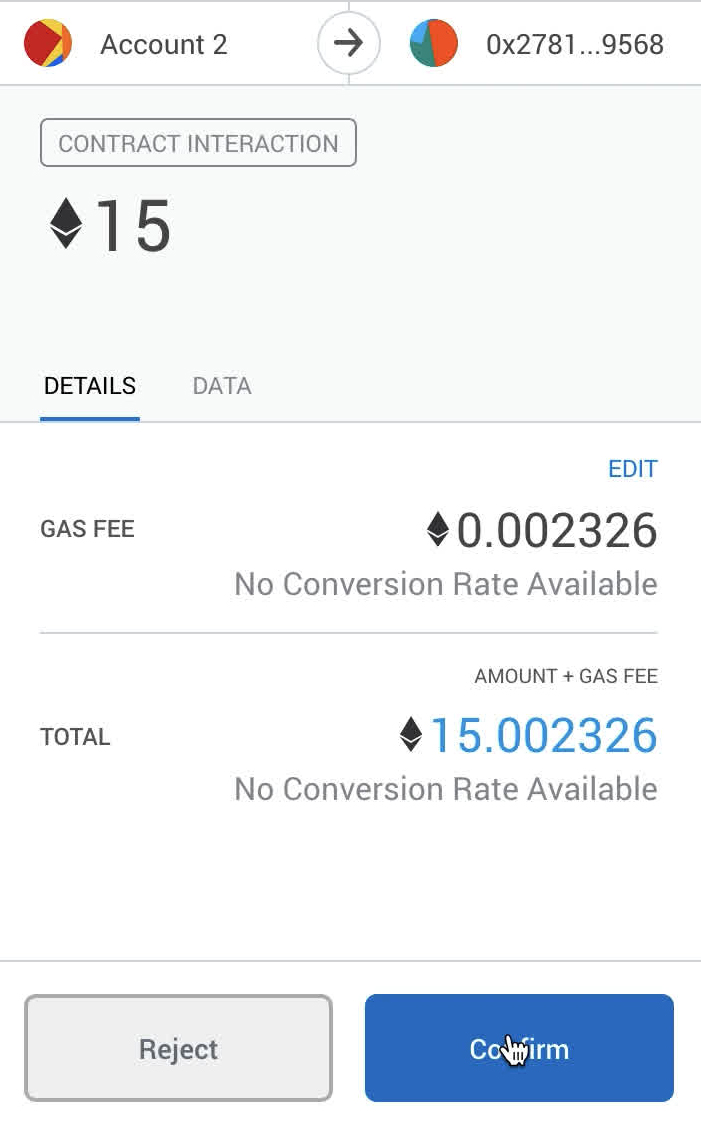
\includegraphics[height=7cm]{graphs/41. alice_metamask_confirm}


\includegraphics[height=7cm]{graphs/42. alice_balance_updated}


\includegraphics[height=7cm]{graphs/43. bob_balance_updated}

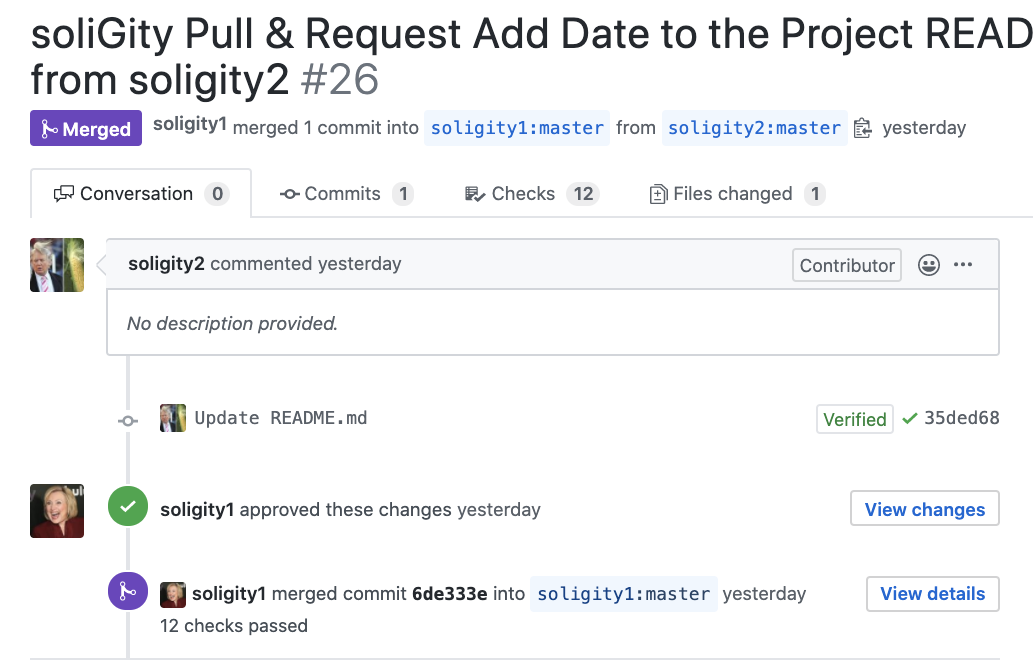
\includegraphics[height=7cm]{graphs/44. pull_request_closed}

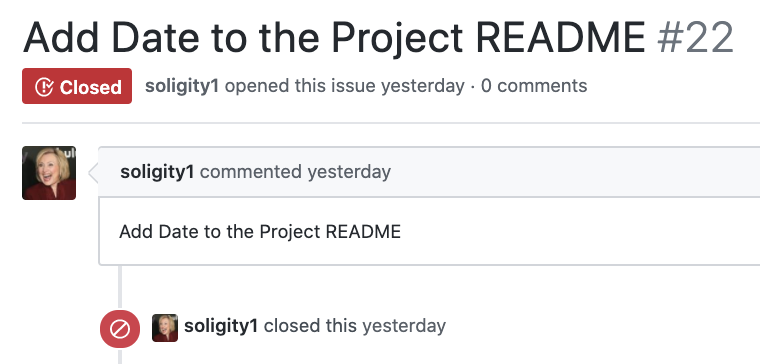
\includegraphics[height=7cm]{graphs/45. issue_closed}

 %%%%%%%%%%%%  Starting New Page here %%%%%%%%%%%%%%

\newpage

\end{enumerate}\par

\textbf{Course Project Team Form}\par


\vspace{\baselineskip}
\begin{Center}
EECE 571G 
\end{Center}\par

\begin{Center}
Blockchain Software Engineering
\end{Center}\par

\begin{Center}
The University of British Columbia
\end{Center}\par


\vspace{\baselineskip}
\begin{Center}
Team\ Name: \_\_\_\_\_\_\_\_\_\_\_\_\_\_\_ 
\end{Center}\par


\vspace{\baselineskip}




\vspace{\baselineskip}



\newpage

\vspace{\baselineskip}
\vspace{\baselineskip}
\textbf{Course Project Peer-to-Peer Evaluation Form}\par


\vspace{\baselineskip}
\begin{Center}
EECE 571G 
\end{Center}\par

\begin{Center}
Blockchain Software Engineering
\end{Center}\par

\begin{Center}
The University of British Columbia
\end{Center}\par


\vspace{\baselineskip}
\begin{Center}
Team\ Name: \_\_\_\_\_\_\_\_\_\_\_\_\_\_\_ 
\end{Center}\par


\vspace{\baselineskip}




\vspace{\baselineskip}

\printbibliography
\end{document}